% ============================================================
% main.tex — documento principale della tesi
%
% Compilazione (da dentro latex-thesis/):
%   latexmk -pdf -bibtex main.tex
% ============================================================
% \documentclass[a4paper,twoside,openright,12pt]{report}
\documentclass[a4paper,twoside,12pt]{report}

% ============================================================
% preamble.tex — pacchetti e configurazione del documento
% ============================================================

% --- Codifica e lingua ---
\usepackage[utf8]{inputenc}
\usepackage[T1]{fontenc}
\usepackage[italian]{babel}
\usepackage{csquotes}

% --- Layout di pagina ---
\usepackage[a4paper,margin=3cm]{geometry}
\usepackage{setspace}
\onehalfspacing
\raggedbottom % evita che flushbottom (default per twoside) stiri gli spazi elastici tra paragrafi/voci di lista per riempire ogni pagina alla stessa altezza
\interfootnotelinepenalty=10000 % vieta lo spezzamento di una nota a piè di pagina tra due pagine

% Layout a due facciate (documentclass in main.tex ha le opzioni
% twoside,openright): i capitoli si aprono su pagina dispari; se serve
% inserire una pagina bianca per arrivarci, la si vuole senza intestazione
% né numero. \cleardoublepage esiste già nel kernel di LaTeX ma non
% sopprime lo stile pagina sulla pagina bianca iniettata: qui si
% ridefinisce per farlo, così una pagina bianca resta visivamente vuota.
\makeatletter
\renewcommand{\cleardoublepage}{%
  \clearpage
  \if@twoside
    \ifodd\c@page\else
      \hbox{}
      \vspace*{\fill}
      \thispagestyle{empty}
      \newpage
    \fi
  \fi
}
\makeatother

% --- Matematica ---
\usepackage{amsmath}
\usepackage{amssymb}
\usepackage{amsthm}
\usepackage{mathtools}

% --- Liste ---
\usepackage{enumitem} % style=nextline per description con etichette lunghe (nomi di file)

% --- Alberi di directory (Unicode box-drawing, es. Panoramica del progetto) ---
% fancyvrb per un blocco verbatim con cornice, senza passare da minted/Pygments
% (che non riconosce i caratteri di disegno delle linee); pmboxdraw insegna a
% pdfLaTeX a disegnarli come regoli vettoriali, dato che non fanno parte dei
% font Latin Modern.
\usepackage{fancyvrb}
\usepackage{pmboxdraw}

% --- Figure e tabelle ---
\usepackage{graphicx}
\usepackage{float} % [H] per la Tabella 3.1, per evitare che il float si separi dal paragrafo che la introduce
\usepackage{booktabs}
\usepackage{siunitx}
\usepackage{caption}
\captionsetup{font=footnotesize}
\usepackage{subcaption}
\usepackage{tikz}
\usetikzlibrary{positioning}

% --- Algoritmi (utile per Cap. 2-3-6: eigensolver, message passing, training loop) ---
\usepackage{algorithm}
\usepackage{algpseudocode}
% babel non traduce il float degli algoritmi né le parole chiave di algpseudocode
\floatname{algorithm}{Algoritmo}
\numberwithin{algorithm}{chapter}
\algrenewcommand\algorithmicrequire{\textbf{Input:}}
\algrenewcommand\algorithmicensure{\textbf{Output:}}
\algrenewcommand\algorithmicfor{\textbf{per}}
\algrenewcommand\algorithmicdo{\textbf{esegui}}
\algrenewcommand\algorithmicend{\textbf{fine}}
\algrenewcommand\algorithmicreturn{\textbf{restituisci}}

% --- Codice sorgente (snippet Python dal progetto, dal Cap. 1 in poi) ---
% Richiede la compilazione con `latexmk -pdf -bibtex -shell-escape main.tex`
% (Pygments/pygmentize deve essere raggiungibile dal PATH). Su Overleaf non
% serve alcuna configurazione: shell-escape per minted è abilitato in automatico.
\usepackage{minted}
\usemintedstyle{default}
\setminted{
    fontsize=\small,
    breaklines,
    tabsize=4,
    frame=none,
    % FancyVrb (usato da minted) apre e chiude l'ambiente con uno spazio verticale
    % calcolato da \topsep/\partopsep (le stesse dimensioni di un ambiente 'list'),
    % non nullo per default: misurato ~13pt su entrambi i lati, ma nel float
    % "listing" solo quello in chiusura restava visibile (quello in apertura viene
    % assorbito dalla riga sotto la caption), dando l'impressione di una riga
    % bianca residua in fondo al blocco. Si azzerano qui entrambi.
    listparameters={\setlength{\topsep}{0pt}\setlength{\partopsep}{0pt}},
}

% Ambiente flottante "Listing" in stile ruled, come nel template UniBa: sostituisce
% il riquadro chiuso (frame=single) usato in precedenza. Numerazione per capitolo,
% come figure e tabelle. Usa il pacchetto float già caricato sopra.
\floatstyle{ruled}
\newfloat{listing}{htbp}{lol}
\floatname{listing}{Listing}
\usepackage{chngcntr}
\counterwithin{listing}{chapter}
% Stile ruled senza la riga orizzontale sopra la caption (resta solo quella tra
% caption e codice, e quella di chiusura in fondo al blocco). \fs@ruled è definito
% da float.sty; qui si ridefinisce solo \@fs@pre come vuoto, il resto invariato.
\makeatletter
\renewcommand\fs@ruled{%
    \def\@fs@cfont{\bfseries}\let\@fs@capt\floatc@ruled
    \def\@fs@pre{}%
    \def\@fs@post{\kern2pt\hrule\relax}%
    \def\@fs@mid{\kern2pt\hrule\kern2pt}%
    \let\@fs@iftopcapt\iftrue}
\makeatother
\captionsetup[listing]{justification=centering, singlelinecheck=false}
\newenvironment{longlisting}[2]{%
    \par\addvspace{\intextsep}%
    \vskip 0pt plus 8\baselineskip\penalty-100\vskip 0pt plus -8\baselineskip
    \captionsetup{type=listing, labelfont=bf, labelsep=space, strut=off,
        aboveskip=0pt, belowskip=0pt}%
    \caption{#1}\label{#2}%
    \nobreak\kern2pt\hrule\kern2pt\nobreak
}{%
    \par\nobreak\kern2pt\hrule\relax
    \par\addvspace{\intextsep}%
}

% --- Bibliografia ---
\usepackage[
    backend=biber,
    style=numeric,
    sorting=nyt
]{biblatex}
\addbibresource{bibliography/references.bib}

% --- Riferimenti incrociati e link (va caricato quasi per ultimo) ---
\usepackage{hyperref}
\hypersetup{
    colorlinks=true,
    allcolors=black,
    bookmarksnumbered=true
}
\usepackage[capitalize,noabbrev]{cleveref}
\crefname{chapter}{Capitolo}{Capitoli}
\Crefname{chapter}{Capitolo}{Capitoli}
\crefname{section}{Sezione}{Sezioni}
\Crefname{section}{Sezione}{Sezioni}
\crefname{algorithm}{Algoritmo}{Algoritmi}
\Crefname{algorithm}{Algoritmo}{Algoritmi}
\crefname{figure}{Figura}{Figure}
\Crefname{figure}{Figura}{Figure}
\crefname{table}{Tabella}{Tabelle}
\Crefname{table}{Tabella}{Tabelle}
\crefname{listing}{Listing}{Listing}
\Crefname{listing}{Listing}{Listing}
\crefname{equation}{equazione}{equazioni}
\Crefname{equation}{Equazione}{Equazioni}
% cleveref non localizza le congiunzioni tra riferimenti multipli (\cref{a,b});
% i comandi non esistono finché cleveref stesso non li definisce a inizio documento,
% quindi la ridefinizione va accodata con \AtBeginDocument per essere eseguita dopo.
\AtBeginDocument{%
  \renewcommand{\crefpairconjunction}{ e }%
  \renewcommand{\crefmiddleconjunction}{, }%
  \renewcommand{\creflastconjunction}{ e }%
  \renewcommand{\crefrangeconjunction}{--}%
}

% --- Ambienti per definizioni/teoremi/proposizioni (utili nei Cap. 2-3) ---
% Gli ambienti condividono la numerazione della sezione "definition"; senza
% aliascnt, cleveref userebbe il nome del contatore e stamperebbe "Definition"
% anche per proposizioni, teoremi, esempi e osservazioni.
\usepackage{aliascnt}
\theoremstyle{definition}
\newtheorem{definition}{Definizione}[chapter]
\newaliascnt{proposition}{definition}
\newtheorem{proposition}[proposition]{Proposizione}
\aliascntresetthe{proposition}
\newaliascnt{theorem}{definition}
\newtheorem{theorem}[theorem]{Teorema}
\aliascntresetthe{theorem}
\newaliascnt{example}{definition}
\newtheorem{example}[example]{Esempio}
\aliascntresetthe{example}
\newaliascnt{remark}{definition}
\newtheorem{remark}[remark]{Osservazione}
\aliascntresetthe{remark}
\renewcommand{\proofname}{Dimostrazione}
\crefname{definition}{Definizione}{Definizioni}
\Crefname{definition}{Definizione}{Definizioni}
\crefname{proposition}{Proposizione}{Proposizioni}
\Crefname{proposition}{Proposizione}{Proposizioni}
\crefname{theorem}{Teorema}{Teoremi}
\Crefname{theorem}{Teorema}{Teoremi}
\crefname{example}{Esempio}{Esempi}
\Crefname{example}{Esempio}{Esempi}
\crefname{remark}{Osservazione}{Osservazioni}
\Crefname{remark}{Osservazione}{Osservazioni}


\title{Graph Neural Network per la previsione multi-asset di
    criptovalute}
\author{}
\date{}

\begin{document}

% ============================================================
% titlepage.tex — frontespizio
% ============================================================
\begin{titlepage}
    \centering

    
\includegraphics[width=0.6\textwidth]{figures/uniba.pdf} \par
    \vspace{0.8cm}

    {\large Dipartimento di Informatica \par}
    \vspace{0.5cm}
    {\large Corso di Laurea in Informatica \par}

    \vspace{1.5cm}
    {\large Tesi di Laurea in Calcolo Numerico \par}

    \vspace{1.5cm}
    {\Large \bfseries Graph Neural Network per la previsione multi-asset di
        criptovalute \par}

    \vspace{2.5cm}
    \begin{minipage}[t]{0.45\textwidth}
        \raggedright
        {\large Relatori:\par}
        {\large \textbf{Francesca Mazzia} \par}
        {\large \textbf{Felice Iavernaro} \par}
    \end{minipage}
    \hfill
    \begin{minipage}[t]{0.45\textwidth}
        \raggedleft
        {\large Candidato:\par}
        {\large \textbf{Giuseppe Guanti} \par}
    \end{minipage}

    \vfill
    {\large Anno Accademico 2025--2026 \par}

\end{titlepage}

\cleardoublepage

\pagenumbering{roman}

% ============================================================
% disclaimer.tex — disclaimer su marchi, nomi commerciali e loghi
% ============================================================
\chapter*{Disclaimer}
\addcontentsline{toc}{chapter}{Disclaimer}

Tutti i marchi, nomi commerciali, prodotti e loghi menzionati in questo elaborato sono di proprietà dei rispettivi titolari.
L'autore non rivendica alcun diritto su tali marchi o nomi commerciali e li utilizza esclusivamente a scopo informativo e descrittivo, senza alcun intento di violazione.


% ============================================================
% ai-statement.tex — dichiarazione sull'uso dell'intelligenza artificiale
% ============================================================
\chapter*{Dichiarazione sull'uso dell'IA}
\addcontentsline{toc}{chapter}{Dichiarazione sull'uso dell'IA}

% Icone inline alte quanto le maiuscole; \mbox impedisce di separare icona e nome a fine riga.
\newcommand{\claudelogo}{\raisebox{-0.15ex}{
\includegraphics[height=1.8ex]{figures/claude-symbol.png}}\,}
\newcommand{\claudecodelogo}{\raisebox{-0.1ex}{
\includegraphics[height=1.5ex]{figures/claude-code-symbol.png}}\,}

Nella realizzazione di questo elaborato sono stati impiegati i modelli linguistici \mbox{\claudelogo Claude} Sonnet~5, \mbox{\claudelogo Claude} Opus~5 e \mbox{\claudelogo Claude} Opus~5.5, anche tramite l'assistente di programmazione \mbox{\claudecodelogo Claude} Code. Tali strumenti sono stati utilizzati per la revisione sintattica del testo, per la generazione delle \cref{fig:graph-filtering,fig:tc-adam-vs-gd} e per la semplificazione di alcune funzioni del codice sperimentale.
Ogni contenuto così ottenuto è stato verificato dall'autore, che ne resta l'unico responsabile.


\chapter*{Sommario}
\addcontentsline{toc}{chapter}{Sommario}

Il mercato delle criptovalute si comporta come un sistema interconnesso: i rendimenti dei diversi asset tendono a muoversi insieme e la loro dipendenza si intensifica nei periodi di crisi. I modelli univariati ignorano per costruzione questa dipendenza, mentre il modello autoregressivo vettoriale (VAR) la rappresenta al prezzo di un numero di parametri che cresce quadraticamente con il numero di asset. La tesi si pone due questioni. La prima è quale vantaggio predittivo offra la struttura relazionale tra criptovalute, sfruttata da una Graph Neural Network, rispetto ad un approccio che le tratti come asset indipendenti; la seconda è come tale struttura si trasformi nel passaggio da un mercato stabile ad uno di crisi.

Il mercato è rappresentato come un grafo dinamico, ricostruito su una finestra mobile dalla correlazione dei rendimenti giornalieri di quindici criptovalute quotate su Binance tra il 2021 e il 2026. Una Graph Convolutional Network (GCN) è confrontata con modelli naive, autoregressivi e VAR e con una propria variante priva di grafo, tramite test di significatività statistica e un backtest al netto dei costi di transazione. L'evoluzione del grafo è misurata con metriche spettrali e topologiche attorno alla stretta regolamentare cinese del 2021, al crollo di Terra/Luna e al fallimento di FTX del 2022.

Quanto alla prima questione, nessun modello supera in modo significativo la previsione nulla e la GCN non si distingue dalla propria variante senza grafo. Il vantaggio che la strategia basata sulle sue previsioni mostra a costo nullo scompare già con una commissione di 10 punti base per cambio di posizione. Quanto alla seconda, il mercato risulta compatto per quasi tutto il periodo: oltre al modo comune a tutti gli asset, la matrice di correlazione non contiene struttura distinguibile dal rumore di stima. La stretta del 2021 porta quasi ogni metrica ad un estremo della propria distribuzione storica, mentre le crisi del 2022 le spostano solo marginalmente, perché investono un mercato già prossimo al suo stato di massima coesione. Nel campione analizzato la struttura relazionale coincide dunque in larga parte con il movimento comune del mercato e, alla frequenza giornaliera e ad un passo, non produce né un vantaggio predittivo né uno economico.


\tableofcontents

% ============================================================
% acronyms.tex — elenco degli acronimi utilizzati nella tesi
%
% Aggiornare manualmente ogni volta che un nuovo acronimo compare
% per la prima volta, in ordine alfabetico.
% ============================================================
\chapter*{Elenco degli acronimi}
\addcontentsline{toc}{chapter}{Elenco degli acronimi}

\begin{description}
    \item[ADA] Cardano
    \item[AR] Autoregressive
    \item[AVAX] Avalanche
    \item[BCH] Bitcoin Cash
    \item[BIC] Bayesian Information Criterion
    \item[BNB] Binance Coin
    \item[BTC] Bitcoin
    \item[DM] Diebold-Mariano
    \item[DOGE] Dogecoin
    \item[DOT] Polkadot
    \item[ETC] Ethereum Classic
    \item[ETH] Ethereum
    \item[FWER] Family-Wise Error Rate
    \item[GAT] Graph Attention Network
    \item[GCN] Graph Convolutional Network
    \item[GNN] Graph Neural Network
    \item[LINK] Chainlink
    \item[LTC] Litecoin
    \item[MAE] Mean Absolute Error
    \item[MLP] Multilayer Perceptron
    \item[MSE] Mean Squared Error
    \item[MST] Minimum Spanning Tree
    \item[OHLCV] Open-High-Low-Close-Volume
    \item[OLS] Ordinary Least Squares
    \item[PMFG] Planar Maximally Filtered Graph
    \item[ReLU] Rectified Linear Unit
    \item[RMSE] Root Mean Square Error
    \item[SOL] Solana
    \item[TRX] TRON
    \item[USDT] Tether
    \item[UST] TerraUSD
    \item[VAR] Vector Autoregression
    \item[XLM] Stellar
    \item[XRP] Ripple
\end{description}


\cleardoublepage
\pagenumbering{arabic}
\setcounter{page}{1}

\chapter*{Introduzione}
\addcontentsline{toc}{chapter}{Introduzione}
\label{ch:introduction}

\let\oldthesection\thesection
\renewcommand{\thesection}{\arabic{section}}

\section{Il mercato delle criptovalute come sistema interconnesso}
\label{sec:crypto-market-interconnected}

Il mercato delle criptovalute appare, ad un primo sguardo, come un insieme ampio ed eterogeneo di asset indipendenti: migliaia di token, ciascuno con una propria tecnologia sottostante, una propria comunità di sviluppatori e un proprio caso d'uso dichiarato. Le serie storiche dei prezzi raccontano una storia diversa. I rendimenti delle criptovalute tendono a muoversi insieme~\cite{ji2019dynamic}. Se gli asset non sono indipendenti, un modello che li tratti come tali sta scartando per costruzione un'informazione potenzialmente rilevante.

Bitcoin resta il nodo dominante di questa rete di dipendenze: pur avendo perso quota di capitalizzazione rispetto ai primi anni del mercato, la sua traiettoria di prezzo continua ad anticipare quella della maggior parte degli \enquote{altcoin}\footnote{Con \enquote{altcoin} (da \emph{alternative coin}) si indica genericamente ogni criptovaluta diversa da Bitcoin.}, che mostrano tipicamente una sensibilità elevata ai suoi movimenti. Gli studi sulla connettività dinamica tra criptovalute, basati sul framework dello \emph{spillover index}\footnote{Indice proposto da Diebold e Yilmaz per misurare quanta parte della varianza dei rendimenti di un asset sia spiegata da shock — variazioni improvvise e inattese dei rendimenti — originati su altri asset, distinguendo chi genera shock netti (fonte) da chi li assorbe (ricevitore)~\cite{dieboldyilmaz2012spillover}.}, confermano questo ruolo. Ad esempio, analizzando il periodo 2015--2018, \textcite{ji2019dynamic} individuano Bitcoin e Litecoin come le principali fonti nette di shock all'interno della rete considerata, mentre la maggior parte degli altcoin si comporta da ricevitore netto.

L'evidenza più chiara di questa interdipendenza emerge nei momenti di crisi, quando le correlazioni tra asset si intensificano invece di attenuarsi. Tre episodi recenti confermano questa dinamica. Nel maggio 2021 l'inasprimento delle restrizioni cinesi su scambi e mining provocò un crollo generalizzato del mercato, con perdite giornaliere medie superiori al 30\% sui principali asset. Un anno dopo, il collasso dell'ecosistema Terra/Luna, legato alla stablecoin algoritmica UST\footnote{Criptovaluta progettata per mantenere un valore stabile, tipicamente ancorato a una valuta come il dollaro statunitense, tramite riserve di collaterale o meccanismi algoritmici.}, cancellò gran parte della capitalizzazione dell'ecosistema in pochi giorni. Questo crollo ebbe conseguenze verificabili anche sulla struttura della rete di correlazione tra criptovalute ad alta capitalizzazione non direttamente coinvolte~\cite{briola2023anatomy}. Nel novembre 2022, il fallimento dell'exchange FTX produsse effetti analoghi sulla connettività tra asset privi di qualunque legame operativo diretto con l'exchange~\cite{akyildirim2023understanding}.

Questi episodi mostrano che le serie di prezzo delle criptovalute non sono indipendenti e che il grado di questa dipendenza non è stabile nel tempo. Le correlazioni tra asset si intensificano nei periodi di crisi e si allentano in quelli di relativa stabilità~\cite{onnela2003dynamics}, in linea con il \emph{volatility clustering} (\cref{sec:stylized-facts})~\cite{cont2001empirical}. Trattare ogni criptovaluta come indipendente dalle altre comporta la perdita di un'informazione potenzialmente rilevante.

\section{Limiti degli approcci classici}
\label{sec:limits-univariate-models}

La famiglia di modelli più diffusa per la previsione di serie storiche finanziarie affronta il problema in modo univariato: un modello AR viene addestrato separatamente su ciascun asset, utilizzando come unico input la storia passata dell'asset stesso~\cite{tsay2010analysis}. Questo approccio tratta ogni criptovaluta come un sistema chiuso, isolato dal resto del mercato: per costruzione, il modello non ha accesso ad alcuna informazione sulle altre serie e non può quindi rappresentare esplicitamente la dipendenza tra asset. Un modello univariato applicato a Bitcoin, ad esempio, non può in linea di principio \enquote{vedere} un segnale di stress che si sta propagando da un'altra parte del mercato, non essendo quel segnale tra i suoi input.

Questo limite si traduce direttamente nell'incapacità di anticipare i fenomeni di contagio discussi nella \cref{sec:crypto-market-interconnected}. Una collezione di modelli univariati indipendenti non può rappresentare l'intensificarsi delle correlazioni durante una crisi, perché tale intensificazione è una proprietà collettiva del sistema di asset, non un tratto osservabile nella singola serie presa da sola.

La statistica multivariata classica offre una risposta parziale a questo problema con il modello VAR, in cui il vettore dei rendimenti di tutti gli asset al tempo $t$ viene regredito sui propri valori ritardati~\cite{lutkepohl2005new}. A differenza dei modelli univariati, un VAR cattura esplicitamente le relazioni tra serie: ogni asset è messo in relazione con il passato di tutti gli altri, non solo con il proprio. Il prezzo di questa espressività è tuttavia alto. Per un sistema di $N$ asset e un ordine di ritardo $p$, il numero di parametri da stimare cresce come $O(N^2 p)$. Con poche decine di criptovalute il numero di parametri diventa rapidamente ingestibile rispetto alla quantità di dati storici disponibili. Ne derivano stime instabili e un rischio di overfitting severo, che rende il VAR classico poco praticabile su un universo ampio ed eterogeneo di asset. Esistono estensioni che attenuano il problema, come i VAR regolarizzati che impongono sparsità sui coefficienti~\cite{basu2015regularized}, ma restano ancorate ad una struttura di dipendenza globale e fissa, incapace di adattarsi ad una topologia di connessioni che cambia nel tempo.

I modelli univariati hanno quindi un costo che cresce linearmente con il numero di asset, ignorandone per costruzione la dipendenza reciproca; il VAR, invece, cattura questa dipendenza, ma con un costo che cresce quadraticamente. Occorre pertanto individuare una struttura capace di rappresentare le relazioni tra criptovalute ad un costo computazionale più sostenibile.

\section{Il grafo come intuizione strutturale}
\label{sec:why-graph-intuition}

Il mercato delle criptovalute, inteso come sistema di asset connessi, si formalizza come grafo pesato: ciascuna criptovaluta è rappresentata da un nodo, ogni coppia di asset è collegata da un arco il cui peso misura l'intensità della relazione tra le due serie, e a ciascun nodo è associato un insieme di feature osservate nel tempo, come rendimento e volume.

Il grafo completo, con un arco per ogni coppia di asset, è però denso e per questo poco trattabile. L'econofisico Mantegna propose per primo un metodo per isolare, a partire dalla matrice di correlazione, le relazioni più significative tra gli asset: un albero di copertura minimo (\emph{minimum spanning tree}, MST) che consente di ottenere una rappresentazione sintetica della struttura di dipendenza del mercato~\cite{mantegna1999hierarchical}. Tecniche successive, sviluppate da Tumminello, raffinano questo filtraggio conservando un numero maggiore di connessioni rilevanti rispetto al solo albero minimo, restituendo una rappresentazione più ricca della struttura di correlazione originale~\cite{tumminello2005tool}.

Mantenere solo le connessioni più rilevanti, principio comune a queste due tecniche, risolve la tensione tra espressività e costo quadratico. Un grafo può restare sparso, includendo un arco solo tra le coppie di asset la cui relazione supera una soglia prefissata, piuttosto che stimare un coefficiente per ogni possibile coppia come richiesto dal VAR completo. Il costo computazionale e statistico dipende quindi esclusivamente dal numero di connessioni effettivamente presenti. Ogni nodo, inoltre, pur conservando una propria dinamica individuale, scambia informazioni con i nodi a cui è connesso attraverso gli archi del grafo. Questa rappresentazione selettiva delle dipendenze, tuttavia, perde di efficacia nei momenti di crisi, quando le connessioni si moltiplicano e la distinzione tra relazioni rilevanti e trascurabili tende a svanire. Il grafo va quindi inteso come una struttura dinamica, con densità variabile nel tempo.

Rappresentare il mercato come un grafo non è però sufficiente a renderlo predittivo: descriverne la topologia in un dato istante non equivale ad un meccanismo per apprendere da questa struttura e trasformarla in una previsione. È necessaria un'architettura capace di elaborare il segnale di ogni nodo tenendo conto, in modo esplicito, dell'assetto del grafo che lo circonda.

\section{Domande di ricerca e struttura della tesi}
\label{sec:objectives-research-questions}

La tesi si articola attorno a due questioni aperte, emerse dalle sezioni precedenti: quale vantaggio predittivo offra la struttura relazionale delle criptovalute rispetto ad un approccio che le tratti come asset indipendenti e come si trasformi la topologia del grafo nel passaggio da un regime di mercato stabile a uno di crisi.

Dal punto di vista teorico, la tesi affronta la prima questione costruendo l'apparato matematico necessario a definire una Graph Convolutional Network in grado di sfruttare la struttura relazionale discussa nella \cref{sec:why-graph-intuition}. Sul piano empirico, la prima questione trova risposta nel \cref{ch:training-and-comparison}, in cui le prestazioni della GCN sono confrontate con quelle delle baseline di riferimento, e nel \cref{ch:backtest}, che ne valuta il vantaggio sul piano economico. La seconda questione viene trattata nel \cref{ch:topological-evolution}, che analizza l'evoluzione della struttura relazionale attorno a tre eventi di crisi.

La tesi è organizzata come segue. Una breve panoramica precede il primo capitolo, presentando l'organizzazione del progetto software su cui si basano i riferimenti al codice nei capitoli successivi. Il \Cref{ch:graph-laplacian-theory} introduce gli strumenti di teoria dei grafi necessari allo studio. Il \Cref{ch:forecasting-models} deriva l'architettura della Graph Convolutional Network di Kipf \& Welling e le baseline con cui viene confrontata. Il \Cref{ch:dynamic-correlation-graph} formalizza la costruzione del grafo dinamico di correlazione a partire dalle serie storiche dei rendimenti. Il \Cref{ch:topological-evolution} applica gli strumenti spettrali alla serie storica del grafo così costruito, misurandone l'evoluzione attorno a tre eventi di crisi reali. Il \Cref{ch:training-and-comparison} descrive l'addestramento dei modelli secondo il protocollo walk-forward e ne confronta le prestazioni tramite skill score e test di significatività statistica. Il \Cref{ch:backtest} valuta le previsioni sul piano economico, con una strategia di trading elementare al netto dei costi di transazione. Il \Cref{ch:conclusions} sintetizza infine i risultati rispetto alle due questioni presentate, discutendone limiti e possibili sviluppi futuri.

\let\thesection\oldthesection

\chapter*{Panoramica del progetto}
\addcontentsline{toc}{chapter}{Panoramica del progetto}
\label{ch:project-overview}

\let\oldthesection\thesection
\let\oldtheHsection\theHsection
\renewcommand{\thesection}{\arabic{section}}
\renewcommand{\theHsection}{po.\arabic{section}}
\setcounter{section}{0}

\section{Struttura del progetto}
\label{sec:project-structure}

Come fatto presente nell'Introduzione, le questioni di ricerca trovano risposta empirica nel progetto software \texttt{cryptognn}, che offre un riscontro diretto, nei capitoli che seguono, alla teoria matematica e alla letteratura econofisica. Lo studio, implementato in Python, vive in script che guidano la pipeline sperimentale e che, per separazione delle responsabilità, si occupano ciascuno di una parte diversa del progetto:

\begin{itemize}
    \item \path{01_download_data.py}. Scarica l'universo di 15 asset da Binance, con cache idempotente su disco.
    \item \path{02_build_graphs.py}. Costruisce il pannello dei prezzi e dei rendimenti, calcola i fatti stilizzati, il tensore di correlazione mobile, calibra la soglia $\tau$ e costruisce i grafi consumati a valle.
    \item \path{03_topology_analysis.py}. Riduce ogni finestra di correlazione alle metriche scalari che ne descrivono la struttura e ne analizza l'andamento in corrispondenza delle tre date di crisi accennate nell'Introduzione.
    \item \path{04_run_baselines.py}. Esegue le baseline di confronto attraverso il protocollo di validazione walk-forward.
    \item \path{05_run_gcn.py}. Esegue la GCN e la sua ablation senza grafo sulla stessa griglia di iperparametri e sugli stessi semi casuali per entrambe le varianti.
    \item \path{06_run_backtest.py}. Trasforma le previsioni di ogni modello in una strategia di trading elementare basata sul segno, valutata a due livelli di costo di transazione.
    \item \path{07_make_figures.py}. Genera tutte le figure della tesi dagli artefatti già prodotti, senza ricalcolare alcun risultato.
    \item \path{08_make_tables.py}. Genera le tabelle, il file di riepilogo con i risultati numerici dello studio e scrive il manifest di riproducibilità, che registra commit, configurazione e hash degli artefatti prodotti così da poter verificare che la stessa configurazione restituisca sempre gli stessi risultati.
\end{itemize}

Ciascuno script si limita ad orchestrare le funzioni definite nei package di \path{src/cryptognn/}. Un'app Streamlit in \path{app/} espone gli stessi artefatti — grafi di correlazione e metriche topologiche — per un'esplorazione interattiva al di fuori della pipeline batch. La struttura del progetto nel suo complesso è la seguente:

\begin{Verbatim}[frame=single, fontsize=\footnotesize]
project-thesis/
├── config/              # file di configurazione dello studio
├── data/                # dati grezzi ed elaborati
├── src/cryptognn/
│   ├── data/            # download e preprocessing delle serie storiche
│   ├── graph/           # grafo di correlazione e metriche topologiche
│   ├── models/          # i modelli previsivi: GCN, VAR, AR, naive
│   └── evaluation/      # protocollo di validazione e backtest
├── scripts/
├── app/                 # app Streamlit
├── results/             # figure, tabelle e metriche dello studio
└── tests/               # suite di test
\end{Verbatim}

\section{Suite di test}
\label{sec:project-tests}

% sloppypar: TestNoLookAhead non è sillababile e altrimenti sborda dal margine.
\begin{sloppypar}
L'affidabilità della pipeline è sostenuta da una suite di $566$ test in \path{tests/}, la cui struttura rispecchia quella di \path{src/cryptognn/}, che verificano il comportamento atteso di ciascun componente nei casi considerati. In particolare, la classe \texttt{TestNoLookAhead} (\path{tests/evaluation/test_walkforward.py}) verifica l'assenza di \emph{look-ahead bias}, ovvero l'uso implicito, durante la previsione, di informazione che a quel momento non sarebbe ancora disponibile. L'errore non farebbe fallire la pipeline, ma renderebbe silenziosamente i risultati migliori di quanto sarebbero in un impiego reale. La relativa logica è discussa nella \cref{sec:tc-walkforward}.
\end{sloppypar}

\let\thesection\oldthesection
\let\theHsection\oldtheHsection

\chapter{Fondamenti matematici: teoria dei grafi e Laplaciano}
\label{ch:graph-laplacian-theory}

\section{Grafi pesati: definizioni e notazione}
\label{sec:weighted-graphs-notation}

L'Introduzione ha motivato l'esigenza di rappresentare esplicitamente le relazioni tra criptovalute, anziché trattare ciascun asset come serie isolata, e la panoramica del progetto appena vista ne ha mostrato il riscontro concreto nella pipeline di \texttt{cryptognn}. Questo capitolo costruisce l'apparato formale su cui quella rappresentazione poggia, muovendo dalla nozione di grafo pesato fino al Laplaciano e alla sua lettura spettrale.
\begin{definition}[Grafo pesato]
\label{def:weighted-graph}
Un grafo pesato è una tripla $G = (V, E, W)$, dove $V = \{v_1, \dots, v_N\}$ è l'insieme dei nodi, $E \subseteq V \times V$ è l'insieme degli archi e $W \in \mathbb{R}^{N \times N}$ è la matrice dei pesi: $w_{ij} \neq 0$ se e solo se $(v_i, v_j) \in E$. Il grafo si assume non orientato e privo di \enquote{self-loop} (archi che collegano un nodo a se stesso): $W$ è simmetrica ($w_{ij} = w_{ji}$) e ha diagonale nulla ($w_{ii} = 0$).
\end{definition}

Quando $w_{ij} \in \{0,1\}$, $W$ coincide con la matrice di adiacenza del grafo non pesato sottostante, che codifica solo la presenza o assenza di un arco, senza informazioni sulla sua intensità. Nel caso generale, $w_{ij}$ misura l'intensità della relazione tra $v_i$ e $v_j$. A partire dal \Cref{ch:dynamic-correlation-graph}, questa intensità sarà la correlazione tra i rendimenti dei due asset. A ciascun nodo si associa un grado\footnote{Il termine \emph{grado} è propriamente riservato al caso non pesato, dove conta il numero di vicini di un nodo; per un grafo pesato la quantità $d_{ii} = \sum_j w_{ij}$ è più propriamente detta \emph{forza} (\emph{strength}) del nodo. Nel seguito si userà comunque \enquote{grado} anche nel caso pesato, per coerenza con la letteratura sulle GCN e con il codice del progetto.}, raccolto nella matrice diagonale $D \in \mathbb{R}^{N\times N}$, $d_{ii} = \sum_{j} w_{ij}$.

Un cammino tra $v_i$ e $v_j$ è una sequenza di nodi $v_i = u_0, u_1, \dots, u_k = v_j$ tale che $(u_{t-1}, u_t) \in E$ per ogni $t = 1, \dots, k$. $G$ è connesso se esiste un cammino tra ogni coppia di nodi e si dice componente connessa un sottoinsieme massimale di nodi mutuamente raggiungibili.

La densità del grafo, cioè il rapporto tra il numero di archi effettivamente presenti e il numero massimo di connessioni possibili tra $N$ nodi, $\binom{N}{2}$, sarà il parametro chiave nel confronto di costo con il VAR (\cref{sec:var-baseline}).

\begin{remark}
\label{rem:negative-weights}
La \Cref{def:weighted-graph} non impone alcun vincolo di segno su $W$. Questo è rilevante perché il peso che si userà nel seguito, ovvero la correlazione di Pearson tra rendimenti, è per costruzione compreso in $[-1,1]$. Sia la semidefinita positività del Laplaciano (\cref{prop:psd}) sia la caratterizzazione della molteplicità dell'autovalore nullo (\cref{prop:zero-multiplicity}) valgono solo sotto l'ipotesi $w_{ij}\geq 0$. La correlazione, però, è per natura un dato con segno: la soluzione sarà proposta nel \Cref{ch:dynamic-correlation-graph}.
\end{remark}

\section{Il Laplaciano del grafo}
\label{sec:graph-laplacian}

Prima di fornirne la definizione formale, è opportuno capire cosa il Laplaciano rappresenti intuitivamente. Ad ogni nodo del grafo si assegna un valore, detto \emph{segnale}. Il Laplaciano confronta il segnale di ogni nodo con quello dei suoi vicini, pesato in base alla forza della connessione, misurando quanto il segnale vari localmente lungo gli archi del grafo, non il valore del segnale stesso. Questa nozione di variazione locale è utile per i seguenti motivi:

\begin{description}
    \item[Diffusione.] Se in un nodo si introduce una perturbazione localizzata — un virus in una rete sociale; il fallimento di una banca in un sistema finanziario — il Laplaciano descrive come e in quanto tempo quella perturbazione si propaga al resto del grafo.
    \item[Gruppi.] Rivela se il grafo si organizza in sottoinsiemi isolati o debolmente connessi tra loro, ovvero gruppi di nodi fittamente collegati al proprio interno e poco collegati verso l'esterno.
    \item[Stabilità.] Misura quanto rapidamente il grafo ritorni in equilibrio dopo una perturbazione localizzata in un punto qualsiasi.
\end{description}

\begin{definition}[Laplaciano del grafo]
\label{def:laplacian}
Il Laplaciano combinatorio di $G$ è la matrice $L = D - W \in \mathbb{R}^{N \times N}$. Si definisce inoltre il Laplaciano normalizzato simmetrico:
$$L_{\mathrm{sym}} = I - D^{-1/2}WD^{-1/2} = D^{-1/2}LD^{-1/2}.$$
\end{definition}

Se i nodi hanno un grado molto eterogeneo, come accade quando Bitcoin è connesso con peso elevato a decine di altcoin mentre un asset minore partecipa ad un numero nettamente minore di collegamenti, il Laplaciano combinatorio $L$ assegna implicitamente più peso ai nodi ad alto grado, distorcendo il confronto tra i loro autovalori. $L_{\mathrm{sym}}$ corregge questa eterogeneità riscalando il peso di ogni arco in base al grado dei due nodi che collega. Nel seguito del capitolo si lavora però con il Laplaciano combinatorio $L$, le cui caratteristiche si dimostrano più direttamente e si trasferiscono, a meno dell'intervallo esatto degli autovalori, a $L_{\mathrm{sym}}$. Si presentano di seguito le proprietà fondamentali del Laplaciano del grafo, formulate rispetto ad un segnale generico $x \in \mathbb{R}^N$.

\begin{proposition}[Forma quadratica del Laplaciano]
\label{prop:quadratic-form}
Per ogni $x \in \mathbb{R}^N$:
$$x^\top L x = \frac{1}{2}\sum_{i,j} w_{ij}(x_i - x_j)^2.$$
\end{proposition}

\begin{proof}
Espandendo il quadrato:
$$\frac12\sum_{i,j}w_{ij}(x_i-x_j)^2 = \frac12\sum_{i,j}w_{ij}x_i^2 - \sum_{i,j}w_{ij}x_ix_j + \frac12\sum_{i,j}w_{ij}x_j^2.$$
Per definizione di $d_{ii}$:
$$\sum_{i,j}w_{ij}x_i^2 = \sum_i x_i^2 \sum_j w_{ij} = \sum_i d_{ii}x_i^2.$$
Scambiando gli indici di somma e usando la simmetria di $W$:
$$\sum_{i,j}w_{ij}x_j^2 = \sum_{i,j}w_{ji}x_i^2 = \sum_i d_{ii}x_i^2.$$
I due termini quadratici coincidono entrambi con $x^\top Dx$, e la somma si riduce a
\begin{equation*}
x^\top Dx - x^\top Wx = x^\top(D-W)x = x^\top Lx. \qedhere
\end{equation*}
\end{proof}

\begin{proposition}[Semidefinita positività]
\label{prop:psd}
Se $w_{ij}\geq 0$ per ogni arco, allora $L \succeq 0$, cioè tutti gli autovalori di $L$ sono non negativi.
\end{proposition}

\begin{proof}
Ogni addendo $w_{ij}(x_i-x_j)^2$ nella \cref{prop:quadratic-form} è non negativo, quindi $x^\top Lx \geq 0$ per ogni $x$. \qedhere
\end{proof}

Se invece si ammettono pesi negativi, caso segnalato nella \cref{rem:negative-weights}, la somma può contenere addendi negativi: $x^\top Lx$ non è più garantito essere non negativo e la \cref{prop:psd} non si applica. Per evitare questo comportamento, il progetto non utilizza direttamente la correlazione di Pearson $\rho_{ij}$ tra i rendimenti degli asset $i$ e $j$ come peso, ma applica preventivamente la trasformazione di Mantegna~\cite{mantegna1999hierarchical}, ripresa per esteso nel \cref{ch:dynamic-correlation-graph}, che mappa la correlazione — con segno, in $[-1,1]$ — in un peso non negativo compreso in $[0,1]$. Il problema del segno è dunque risolto interamente in fase di costruzione del grafo.

\begin{proposition}[Molteplicità dell'autovalore nullo]
\label{prop:zero-multiplicity}
Sotto l'ipotesi $w_{ij}\geq 0$, ora garantita in pratica dalla trasformazione di Mantegna, la molteplicità dell'autovalore $0$ di $L$ è pari al numero di componenti connesse di $G$.
\end{proposition}

\begin{proof}
Siano $C_1,\dots,C_m$ le componenti connesse di $G$ e $\mathbf{1}_{C_k}\in\mathbb{R}^N$ il vettore indicatore di $C_k$\footnote{Il vettore indicatore (o vettore caratteristico) di un sottoinsieme $C\subseteq V$ è il vettore $\mathbf{1}_C\in\mathbb{R}^N$ le cui componenti valgono $(\mathbf{1}_C)_i=1$ se $v_i\in C$ e $(\mathbf{1}_C)_i=0$ altrimenti.}. Per $i \in C_k$, tutti i vicini di $i$ appartengono a $C_k$ (non essendoci archi tra componenti diverse), quindi $(L\mathbf{1}_{C_k})_i = d_{ii} - \sum_{j} w_{ij}(\mathbf{1}_{C_k})_j = d_{ii} - d_{ii} = 0$; per $i \notin C_k$, sia $(\mathbf{1}_{C_k})_i$ sia ogni $w_{ij}$ con $j \in C_k$ sono nulli. Dunque $L\mathbf{1}_{C_k}=0$ per ogni $k$, e i vettori $\mathbf{1}_{C_1},\dots,\mathbf{1}_{C_m}$, avendo supporti disgiunti, sono linearmente indipendenti: la molteplicità di $0$ è almeno $m$.

Viceversa, sia $x\in\ker(L)$, cioè $Lx=0$: allora $x^\top Lx = x^\top(Lx) = 0$, e la \cref{prop:quadratic-form} impone $w_{ij}(x_i-x_j)^2=0$ per ogni coppia $(i,j)$: dato che i pesi sono non negativi, ciò forza $x_i=x_j$ per ogni arco di peso non nullo, quindi $x$ è costante su ciascuna componente connessa, cioè $x\in\mathrm{span}\{\mathbf{1}_{C_1},\dots,\mathbf{1}_{C_m}\}$. Il nucleo di $L$ è allora esattamente questo spazio, di dimensione $m$: essendo $L$ simmetrico, questa molteplicità geometrica coincide con quella algebrica~\cite{chung1997spectral}. \qedhere
\end{proof}

La forma quadratica misura quanto un segnale $x$ definito sui nodi del grafo sia \enquote{irregolare}, nel senso di assumere valori molto diversi tra nodi fortemente connessi. Un segnale costante su ogni componente ha forma quadratica nulla; un segnale che oscilla bruscamente tra nodi vicini ha forma quadratica elevata. Applicata agli autovettori di $L$ piuttosto che ad un segnale generico, questa nozione di irregolarità suggerisce un'idea di \enquote{frequenza} del grafo.

\section{Analisi spettrale: autovalori e autovettori}
\label{sec:spectral-analysis}

Per rendere precisa l'analogia tra irregolarità di un segnale e frequenza serve un modo per scomporre $L$ nelle sue componenti elementari: autovettori e autovalori.

\begin{theorem}[Decomposizione spettrale del Laplaciano]
\label{thm:spectral-decomposition}
Essendo $L$ simmetrica e reale, esiste una decomposizione
$$L = U\Lambda U^\top,$$
con $U \in \mathbb{R}^{N\times N}$ ortogonale ($U^\top U = I$) le cui colonne $u_1,\dots,u_N$ sono autovettori di $L$ a norma unitaria e $\Lambda = \mathrm{diag}(\lambda_1,\dots,\lambda_N)$ la matrice diagonale dei corrispondenti autovalori, ordinati $0 = \lambda_1 \leq \lambda_2 \leq \dots \leq \lambda_N$ (l'ordinamento a partire da $\lambda_1=0$ segue dalla \cref{prop:psd} e dalla \cref{prop:zero-multiplicity}).
\end{theorem}

Chiamando $\lambda_1,\dots,\lambda_N$ lo spettro di $L$, il \cref{thm:spectral-decomposition} fornisce lo strumento per estendere l'interpretazione della \cref{prop:quadratic-form} da un segnale generico $x$ ad un singolo autovettore $u_k$: poiché il teorema garantisce che ogni $u_k$ abbia norma unitaria,
$$\lambda_k = u_k^\top L u_k = \frac12\sum_{i,j}w_{ij}\big(u_k(i)-u_k(j)\big)^2,$$
dove $u_k(i)$ denota la $i$-esima componente di $u_k$. L'autovalore $\lambda_k$ è quindi la misura di irregolarità del proprio autovettore, nel senso fissato nella \cref{sec:graph-laplacian}.

Gli autovettori a basso indice, con $\lambda_k$ piccolo, variano poco tra nodi fortemente connessi e si dicono \emph{modi lisci}; quelli ad alto indice, con $\lambda_k$ grande, oscillano invece bruscamente tra nodi in stretta relazione e prendono il nome di \emph{modi oscillanti}. L'analogia con il concetto di frequenza di un segnale nel tempo è immediata: una bassa frequenza descrive un'onda che varia lentamente; una frequenza elevata un'onda che oscilla rapidamente. In modo analogo, un $\lambda_k$ piccolo corrisponde ad un modo quasi costante sul grafo, mentre un $\lambda_k$ grande rappresenta un modo che cambia segno da un nodo all'altro. Il termine \enquote{frequenza} sarà quindi utilizzato nel seguito per indicare gli autovalori di $L$.

Tra queste frequenze, la prima non banale merita un'attenzione particolare. Assumendo $G$ connesso, la \cref{prop:zero-multiplicity} assegna molteplicità $1$ all'autovalore $\lambda_1=0$. Il modo $u_1$, a irregolarità nulla, è dunque costante su tutto il grafo ed è l'unico a non portare alcuna informazione sulla sua struttura. Il primo autovalore informativo è dunque $\lambda_2$. Quest'ultimo è, tra tutti i segnali non costanti sul grafo, ortogonali al modo costante $u_1$, il valore più piccolo che la forma quadratica della \cref{prop:quadratic-form} può assumere:
$$\lambda_2 = \min_{\substack{x\neq 0 \\ x\perp u_1}} \frac{x^\top Lx}{x^\top x}.$$
In altre parole, qualunque segnale non costante si scelga, la somma pesata delle sue variazioni tra nodi collegati non può mai scendere sotto $\lambda_2$. Questo rende $\lambda_2$ sensibile alla rimozione di un singolo arco $(i,j)$: l'operazione abbassa il valore della forma quadratica di $w_{ij}(x_i-x_j)^2$ per ogni segnale $x$, mentre il vincolo $x\perp u_1$ resta lo stesso, dato che il vettore costante $u_1$ appartiene al nucleo del Laplaciano qualunque siano i pesi (\cref{prop:zero-multiplicity}). Il minimo di una quantità che può solo diminuire, calcolato su un dominio invariato, non può quindi aumentare: $\lambda_2$ non cresce mai per rimozione di un arco. La sua diminuzione, però, non è affatto limitata dal peso dell'arco rimosso: se quell'arco è l'unico a connettere due parti del grafo, la sua rimozione disconnette $G$ e porta $\lambda_2$ esattamente a $0$ (\cref{prop:zero-multiplicity}), per quanto piccolo fosse il suo peso. Se il valore di partenza è invece elevato, portarlo a $0$ richiede la rimozione cumulativa di molti archi. L'autovalore $\lambda_2$ misura quindi quanto il grafo resista alla rimozione di archi: quanto più il suo valore è grande, tanto più risulta difficile disconnetterlo. Per questo motivo, $\lambda_2$ prende il nome di \emph{connettività algebrica}.

L'autovettore $u_2$ associato a $\lambda_2$, detto \emph{vettore di Fiedler}, è il segnale non costante che realizza questo minimo.

Questa logica suggerisce un modo naturale per misurare il compattamento del grafo di correlazione durante i periodi di crisi, tramite un aumento generalizzato di $\lambda_2$ dovuto a connessioni più forti e più diffuse. Nel \Cref{ch:topological-evolution} questa idea viene applicata direttamente alla serie storica del grafo di correlazione del progetto.

\chapter{GCN e baseline}
\label{ch:forecasting-models}

\section{Dal percettrone al layer su grafo}
\label{sec:from-perceptron-to-graph-layer}

Il \Cref{ch:graph-laplacian-theory} ha fornito gli strumenti necessari per descrivere un grafo pesato e quantificarne la connettività tramite il Laplaciano, utilizzati ora per definire un modello che apprende dai dati. Il punto di partenza è il modello neurale più semplice, il percettrone multistrato (\emph{multilayer perceptron}, MLP), che rappresenta l'input come un vettore $h^{(0)}\in\mathbb{R}^{F_0}$ e lo trasforma applicando in sequenza $L$ strati della forma
\begin{equation}
\label{eq:mlp-layer}
h^{(l+1)} = \sigma\!\left(W^{(l)}h^{(l)} + b^{(l)}\right),
\end{equation}
ove $h^{(l)}$ è la rappresentazione del sistema allo strato $l$, $W^{(l)}\in\mathbb{R}^{F_{l+1}\times F_l}$ e $b^{(l)}\in\mathbb{R}^{F_{l+1}}$ sono parametri appresi\footnote{Nel \Cref{ch:graph-laplacian-theory} il simbolo $W$ denota la matrice dei pesi del grafo. $W^{(l)}$ denota invece la matrice dei parametri appresi dallo strato $l$ nelle reti neurali. Nel seguito la distinzione è affidata all'apice: $W$ resta la matrice dei pesi del grafo, $W^{(l)}$ è sempre una matrice di parametri.} e $\sigma$ è una funzione non lineare applicata componente per componente. La non linearità è essenziale: componendo strati puramente lineari si otterrebbe ancora una trasformazione lineare e la profondità non aggiungerebbe alcuna capacità espressiva~\cite{goodfellow2016deep}.

I parametri si stimano minimizzando una funzione di costo $C$ tramite discesa del gradiente, che sposta ciascun peso nella direzione che riduce maggiormente tale costo. Il gradiente $\partial C/\partial W^{(l)}$ misura la sensibilità della funzione $C$ ad una variazione di ogni peso e si calcola tramite backpropagation~\cite{rumelhart1986learning}, l'applicazione sistematica della regola della catena che percorre all'indietro il grafo computazionale definito dalla composizione degli $L$ strati.

Poiché, per l'equazione~\eqref{eq:mlp-layer}, $h^{(l+1)}$ dipende da $h^{(l)}$ solo attraverso lo strato $l+1$, la regola della catena esprime il gradiente rispetto al peso $w^{(l)}_{ij}$ in funzione di quello rispetto a $h^{(l+1)}$ e dello jacobiano dello strato stesso, nella forma esplicita
\begin{equation}
\label{eq:backprop-weight-gradient}
\frac{\partial C}{\partial w^{(l)}_{ij}} = \frac{\partial C}{\partial h^{(l+1)}_i} \cdot \sigma'\!\left(z^{(l+1)}_i\right) \cdot h^{(l)}_j, \qquad z^{(l+1)} = W^{(l)}h^{(l)} + b^{(l)}.
\end{equation}
La backpropagation sfrutta questa struttura calcolando il gradiente a ritroso. Partendo dal gradiente rispetto a $h^{(L)}$, ottenuto direttamente dalla funzione di costo, ogni gradiente rispetto a $h^{(l+1)}$ già noto viene riutilizzato sia per il calcolo del gradiente rispetto a $W^{(l)}$, sia per quello rispetto a $h^{(l)}$. Si prosegue verso gli strati precedenti senza mai ricalcolare da capo il tratto di catena condiviso tra pesi diversi. Il costo dell'intera procedura è noto crescere linearmente con il numero di strati, anziché esplodere con la loro profondità.

\subsection{Le proprietà di una convoluzione su grafo}
\label{sec:message-passing-paradigm}

L'equazione~\eqref{eq:mlp-layer} tratta $h^{(0)}$ come un vettore generico, in cui ogni componente è una coordinata indipendente dalle altre. Il calcolo non tiene conto della struttura del grafo $G=(V,E,W)$ introdotto nel \cref{ch:graph-laplacian-theory}. Un layer che sfrutti questa informazione deve soddisfare tre proprietà:

\begin{description}
    \item[Località.] L'uscita relativa al nodo $v_i$ deve dipendere solo dai valori di $h^{(l)}$ sui nodi a esso adiacenti, non sull'intero grafo: un layer denso, che lascia ogni nodo influenzare l'uscita di ogni altro indipendentemente da $E$, ignorerebbe per intero la struttura appena costruita e richiederebbe $O(N^2)$ parametri ($N$ il numero di nodi, \cref{def:weighted-graph}) anziché sfruttare la sparsità di $E$.
    \item[Condivisione dei pesi.] La trasformazione applicata a ciascun nodo deve essere la stessa per tutti: il grafo di correlazione è ricalcolato a ogni finestra temporale (\cref{sec:dynamic-graphs-temporal-question}), quindi lo stesso layer deve funzionare, senza essere riaddestrato, su realizzazioni diverse del grafo.
    \item[Equivarianza per permutazione.] La numerazione dei nodi $v_1,\dots,v_N$ introdotta nella \cref{def:weighted-graph} è arbitraria, frutto dell'ordine in cui i nodi sono stati elencati e non di una loro proprietà. Permutarla non deve alterare le uscite del layer, solo la loro etichetta.
\end{description}

Una funzione lineare che soddisfa le tre proprietà ha forma:
\begin{equation}
\label{eq:graph-aggregation}
h_i^{(l+1)} = \sigma\!\left(\sum_{v_j \in \mathcal{N}(v_i)} w_{ij}\, W^{(l)} h_j^{(l)}\right),
\end{equation}
ove $\mathcal{N}(v_i) = \{v_j \in V : (v_i,v_j)\in E\}$ denota il vicinato di $v_i$ (\Cref{fig:graph-neighborhood}); $w_{ij}$ sono i pesi del grafo — non appresi, ma fissati dalla struttura di $G$ — e $W^{(l)}$ è la trasformazione appresa, condivisa da ogni nodo $v_i$.

\begin{figure}[H]
\centering
\begin{tikzpicture}[scale=0.72, every node/.style={font=\small}]
    \tikzset{nd/.style={circle, draw, inner sep=0pt, minimum size=5.5pt, fill=white}}
    \node[nd, fill=black, label=below:{$v_i$}] (c) at (2.2,2.1) {};
    \node[nd] (a1) at (0.6,3.3) {};
    \node[nd] (a2) at (1.0,1.0) {};
    \node[nd] (a3) at (3.6,3.1) {};
    \node[nd] (a4) at (3.5,1.1) {};
    \node[nd] (a5) at (2.6,3.9) {};
    \node[nd] (b1) at (0.0,2.0) {};
    \node[nd] (b2) at (4.6,2.2) {};
    \node[nd] (b3) at (1.6,4.5) {};
    \draw[gray!80] (c)--(a1) (c)--(a2) (c)--(a3) (c)--(a4) (c)--(a5);
    \draw[gray!45] (a1)--(b1) (a2)--(b1) (a3)--(b2) (a4)--(b2) (a5)--(b3) (a1)--(b3) (a3)--(a5);
    \node at (2.3,-1.0) {Vicinato $\mathcal{N}(v_i)$};
\end{tikzpicture}
\caption[Vicinato di un nodo su un grafo]{Il vicinato $\mathcal{N}(v_i)$ è un insieme non ordinato e di cardinalità variabile, dipendente dal nodo $v_i$ considerato.}
\label{fig:graph-neighborhood}
\end{figure}

La somma ristretta a $\mathcal{N}(v_i)$ realizza la località; $W^{(l)}$, lo stesso per ogni $i$, realizza la condivisione dei pesi. Quanto all'equivarianza per permutazione, la somma è definita su un insieme di vicini anziché su una sequenza ordinata e dipende da $w_{ij}$ e $h_j^{(l)}$ ma non dagli indici $i,j$ in sé. Rinumerare i nodi permuta di conseguenza $w_{ij}$ e $h_j^{(l)}$, ma lascia $h_i^{(l+1)}$ invariata a parità di nodo fisico~\cite{bronstein2021geometric}.

Si noti che $h_i^{(l+1)}$ non include la rappresentazione precedente del nodo stesso, $h_i^{(l)}$, a meno che $v_i \in \mathcal{N}(v_i)$: la \Cref{sec:gcn-kipf-welling} mostra come la GCN risolva il problema aggiungendo un self-loop a ogni nodo.

\section{La Graph Convolutional Network}
\label{sec:gcn-kipf-welling}

La \cref{sec:from-perceptron-to-graph-layer} ha lasciato aperte due questioni, entrambe implicite nella forma lineare dell'Eq.~\eqref{eq:graph-aggregation}. La prima riprende quanto osservato a chiusura del paragrafo: la somma è ristretta a $\mathcal N(v_i)$, quindi $h_i^{(l+1)}$ non include $h_i^{(l)}$ a meno che $v_i\in\mathcal N(v_i)$ — un nodo, dopo un solo layer, non conserva più alcuna informazione sulla propria rappresentazione precedente. La seconda non è stata ancora discussa: la somma $\sum_j w_{ij}h_j^{(l)}$ non ha alcun vincolo di scala e cresce con il numero e il peso dei vicini di ciascun nodo. Kipf e Welling~\cite{kipf2017gcn} risolvono entrambe le questioni con due correzioni mirate, applicate direttamente alla forma lineare appena derivata, ottenendo la Graph Convolutional Network (GCN).

Si isola momentaneamente la discussione al caso di un solo filtro, con $F_l=F_{l+1}=1$, in cui $W^{(l)}$ si riduce ad uno scalare $\theta$ e $h^{(l)}$ ad un segnale $x\in\mathbb{R}^N$ sui nodi, una restrizione temporanea rimossa successivamente generalizzando a $F$ feature per nodo. Sotto questa restrizione, l'Eq.~\eqref{eq:graph-aggregation} diventa, per ciascun nodo,
$$y_i = \theta\sum_{v_j\in\mathcal N(v_i)}w_{ij}x_j = \theta\,(Wx)_i,$$
ovvero $y=\theta Wx$ in forma matriciale.

La seconda questione riguarda direttamente questo prodotto. $W$ non ha alcun vincolo di scala e un nodo con grado elevato produce una somma di magnitudine maggiore di quella di un nodo periferico, esattamente il problema già incontrato per il Laplaciano nella \cref{sec:graph-laplacian}. Si applica nuovamente la normalizzazione simmetrica $D^{-1/2}(\cdot)D^{-1/2}$ piuttosto che utilizzare la matrice grezza $W$,
$$y = \theta D^{-1/2}WD^{-1/2}x.$$

La prima, invece, è quella lasciata aperta dalla \cref{sec:from-perceptron-to-graph-layer}. La somma normalizzata non include ancora $x_i$, a meno che $v_i$ sia vicino di sé stesso. In caso contrario, il nodo perde ogni contributo diretto della propria rappresentazione. Il modo più diretto per ovviare a questo problema è sommare $x_i$ al risultato, riutilizzando lo stesso $\theta$ già condiviso da ogni vicino invece di introdurre un secondo parametro per il solo termine centrale. Si ottiene così
\begin{equation}
\label{eq:gcn-step3}
y = \theta\left(I + D^{-1/2}WD^{-1/2}\right)x.
\end{equation}

\subsection{Il renormalization trick}

Sottraendo a $2$ lo spettro di $L_{\mathrm{sym}}$, per cui vale $\lambda_{\max}\leq2$~\cite{chung1997spectral}, con uguaglianza se e solo se il grafo ha una componente connessa bipartita\footnote{Un grafo è bipartito se i suoi nodi si dividono in due insiemi e ogni arco collega un nodo del primo a uno del secondo. È un caso non tipico per il grafo di correlazione tra criptovalute di questo studio, dove ogni asset è connesso a molti altri.}, si ottiene lo spettro dell'operatore $I + D^{-1/2}WD^{-1/2}$, contenuto quindi in $[0,2]$. Impilando $l$ layer, l'operatore viene applicato $l$ volte, e le componenti del segnale associate agli autovalori prossimi a $2$ vengono amplificate di un fattore che cresce come $2^l$, con conseguente instabilità numerica e gradienti che esplodono. Kipf e Welling risolvono il problema con il \emph{renormalization trick}. Anziché essere sommato dopo come nell'Eq.~\eqref{eq:gcn-step3}, il self-loop entra nell'adiacenza prima della normalizzazione, ricalcolata sul grafo così modificato,
\begin{equation}
\label{eq:renormalization}
\tilde A = A + I,\qquad \tilde d_{ii}=\sum_j\tilde a_{ij},\qquad \hat A = \tilde D^{-1/2}\tilde A\tilde D^{-1/2},
\end{equation}
dove $A$ denota la matrice di adiacenza, che in questo caso coincide con la matrice $W$ della \cref{def:weighted-graph} essendo il grafo pesato. La sostituzione di $I + D^{-1/2}WD^{-1/2}$ con $\hat A$ non cambia la sostanza dell'operazione (in entrambi i casi ogni nodo combina sé stesso con i propri vicini) ma riporta lo spettro in $[-1,1]$, dove l'applicazione ripetuta non fa crescere l'ampiezza del segnale.

Applicando questa sostituzione e generalizzando l'equazione~\eqref{eq:gcn-step3} da un segnale scalare per nodo a un vettore di $F_l$ feature per nodo — cioè da $x\in\mathbb{R}^N$ a una matrice $H^{(l)}\in\mathbb{R}^{N\times F_l}$ — e da un filtro a $F_{l+1}$ filtri appresi in parallelo, si ottiene infine la regola di propagazione della Graph Convolutional Network (GCN):
\begin{equation}
\label{eq:gcn}
\boxed{\;H^{(l+1)} = \sigma\!\left(\tilde D^{-1/2}\tilde A\tilde D^{-1/2}H^{(l)}W^{(l)} + b^{(l)}\right)\;}
\end{equation}
con $H^{(l)}\in\mathbb{R}^{N\times F_l}$, $W^{(l)}\in\mathbb{R}^{F_l\times F_{l+1}}$, $b^{(l)}\in\mathbb{R}^{F_{l+1}}$ e $\sigma$ non lineare come nell'equazione~\eqref{eq:mlp-layer}, che nell'implementazione dello studio è la ReLU, $\sigma(z)=\max(0,z)$.

\subsection{Lettura della formula}

L'equazione~\eqref{eq:gcn} condensa le correzioni finora discusse.

\begin{description}
    \item[$H^{(l)}$ — Rappresentazioni correnti.] La riga $i$-esima è il vettore di feature del nodo $v_i$ allo strato $l$. Allo strato iniziale $H^{(0)}$ contiene le feature osservate: nel caso del grafo delle criptovalute, sono le grandezze estratte dalla serie storica di ciascun asset (\cref{sec:tc-node-features}).
    \item[$W^{(l)}$ — Trasformazione delle feature.] È una matrice di parametri appresa e condivisa da \emph{tutti} i nodi. Il numero di parametri dipende dalle dimensioni $F_l\times F_{l+1}$ dello spazio delle feature, non da $N$, condivisione dei pesi della \cref{sec:from-perceptron-to-graph-layer}. Un modello addestrato su un grafo può quindi essere applicato ad un grafo con numero diverso di nodi. Si tratta di una proprietà indispensabile per i grafi dinamici della \cref{sec:dynamic-graphs-temporal-question}.
    \item[$\tilde A = A + I$ — Self-loop.] Senza il termine $+I$, l'aggiornamento di un nodo sarebbe funzione dei soli vicini e il nodo perderebbe ad ogni strato la propria informazione: dopo un solo strato la rappresentazione di un asset non conterrebbe più nulla della sua serie storica, ma solo informazioni su quelle delle altre criptovalute. Il self-loop impone che ogni nodo veda anche sé stesso e lo fa senza introdurre un secondo insieme di parametri distinto per il termine centrale.
    \item[$\tilde D^{-1/2}(\cdot)\tilde D^{-1/2}$ — Normalizzazione simmetrica.] Impedisce che i nodi ad alto grado dominino: senza di essa, un nodo connesso a molti altri produrrebbe somme di magnitudine molto maggiore rispetto a nodi periferici, e la rete finirebbe per modellare il grado anziché il segnale. La forma simmetrica $\tilde D^{-1/2}\tilde A\tilde D^{-1/2}$, a differenza della normalizzazione per righe $\tilde D^{-1}\tilde A$, mantiene l'operatore simmetrico e quindi a spettro reale, preservando l'interpretazione spettrale del \Cref{ch:graph-laplacian-theory}. Come già osservato, confina lo spettro in $[-1,1]$ e rende stabile l'impilamento di più strati.
\end{description}

Il coefficiente con cui il nodo $v_j$ contribuisce all'aggiornamento di $v_i$ è dunque $\hat a_{ij} = \tilde a_{ij}/\sqrt{\tilde d_i\tilde d_j}$, con $\tilde d_i = \tilde d_{ii}$, somma pesata in cui il peso decresce con il grado di entrambi gli estremi dell'arco. Questi coefficienti sono \emph{imposti} dalla struttura del grafo e non appresi.

Quanto al costo, l'equazione~\eqref{eq:gcn} si valuta come $\hat A(H^{(l)}W^{(l)})$. La trasformazione delle feature costa $O(NF_lF_{l+1})$ e la propagazione sul grafo, con $\hat A$ in formato sparso, $O(|E|F_{l+1})$. Il costo è dunque lineare nel numero di archi, non quadratico in $N$, a condizione che il grafo sia effettivamente sparso.

La \cref{sec:from-perceptron-to-graph-layer} ha già stabilito che un layer aggrega solo i vicini immediati, la località dell'Eq.~\eqref{eq:graph-aggregation}. In forma matriciale questo si traduce nella struttura di $\hat A$: l'entrata $\hat a_{ij}$ è diversa da zero solo se $(v_i,v_j)\in E$ oppure $i=j$, per costruzione della matrice dei pesi $W$ (\cref{def:weighted-graph}) e del self-loop $\tilde A=A+I$. Il prodotto $(\hat A H^{(l)})_i = \sum_j \hat a_{ij}h_j^{(l)}$ riceve dunque contributo solo dai termini con $j\in\mathcal N(v_i)\cup\{v_i\}$, gli altri sono moltiplicati per zero. Impilando $l$ layer, il campo recettivo si estende a $l$ passi. La GCN ottiene così espressività aumentando la profondità, più strati con pochi parametri ciascuno, invece di allargare il campo recettivo di un singolo strato con più parametri.

\section{Limiti noti delle GNN}
\label{sec:known-limitations-gnn}

Il campo recettivo di una GCN si allarga all'aumentare degli strati impilati. Osservando anche il comportamento delle reti neurali in generale, è naturale aspettarsi che una maggiore profondità porti sempre a una maggiore capacità. In realtà, per i grafi, questa condizione non si verifica.

\subsection{Over-smoothing}
All'aumentare del numero di strati, le rappresentazioni dei nodi tendono a diventare indistinguibili tra loro~\cite{li2018deeper}. Trascurando momentaneamente le non linearità, le trasformazioni $W^{(l)}$ e i bias $b^{(l)}$, impilare $l$ strati GCN equivale ad applicare $\hat A^l$ al segnale di ingresso. Poiché lo spettro di $\hat A$ è contenuto in $[-1,1]$ con autovalore massimo pari a $1$, elevare a potenza schiaccia progressivamente tutte le componenti associate ad autovalori di modulo minore di $1$. Il segnale converge quindi alla proiezione sull'autovettore dominante $\tilde D^{1/2}\mathbf{1}$. Si verifica infatti che $\hat A\tilde D^{1/2}\mathbf1 = \tilde D^{-1/2}\tilde A\mathbf1 = \tilde D^{-1/2}\tilde D\mathbf1 = \tilde D^{1/2}\mathbf1$. È l'analogo, per $\hat A$, di quanto già stabilito nella \cref{prop:zero-multiplicity} per l'autovalore nullo del Laplaciano. Il modo a irregolarità minima non porta informazione strutturale. Questo limite dipende solo dai gradi dei nodi. Le feature di partenza, cioè le differenze tra nodi che il modello dovrebbe sfruttare, non hanno più alcun peso.

\subsection{Grafi densi}
Tutti i vantaggi di costo discussi in questo capitolo sono espressi in funzione di $|E|$ e valgono perché il grafo è sparso. Se $|E|$ si avvicina a $N^2$ il costo $O(|E|F)$ per strato torna quadratico e il vantaggio computazionale svanisce. Su un grafo denso, inoltre, il vicinato a due passi copre già quasi tutti i nodi. L'over-smoothing si manifesta quindi prima, a profondità minore.

Un grafo di correlazione costruito senza filtrare gli archi è per costruzione completo. Il \Cref{ch:dynamic-correlation-graph} affronta la sparsificazione come condizione di funzionamento del modello. Nel grafo di questo studio la soglia calibrata lascia in piedi quasi tutti gli archi, con una densità media di 0,974 che non scende mai sotto 0,733.
La pratica corrente offre una risposta parziale. Le architetture GNN efficaci sui compiti reali usano tipicamente due o tre strati, un campo recettivo modesto che si dimostra preferibile a rappresentazioni più ampie ma rese indistinguibili dall'over-smoothing. La GCN di questo studio applica questa scelta all'estremo inferiore dell'intervallo, con due soli strati e un campo recettivo di due passi, coerente sia con la densità del grafo sia con l'over-smoothing appena discusso.

\section{Baseline}
\label{sec:baselines}

Come termine di paragone per la capacità predittiva della GCN sono state selezionate tre famiglie di modelli che non utilizzano il grafo di correlazione. I modelli naive non guardano le relazioni tra asset o la storia della singola criptovaluta. AR, invece, utilizza esclusivamente la serie storica dell'asset considerato. VAR usa le serie di tutti gli asset senza una struttura esplicita che li leghi.

L'obiettivo di questo confronto è determinare se la struttura relazionale tra criptovalute offre un vantaggio predittivo misurabile rispetto ad un modello che non ne tiene conto. Lo studio tratta questa domanda come una verifica. La baseline di confronto più esigente è quella naive: in finanza la previsione nulla o la media storica battono spesso modelli più sofisticati.

\subsection{Naive}

Un modello naive costituisce un limite inferiore di riferimento per la valutazione di un modello predittivo: non effettua alcuna stima parametrica dai dati, ma restituisce la quantità più elementare disponibile che, nel caso più comune, corrisponde ad un valore costante. La sua funzione non è predittiva in senso proprio, poiché si limita a definire la soglia minima di prestazione che qualunque modello di complessità superiore deve superare per giustificare la propria adozione. Se un modello più sofisticato non supera questo limite, l'apparato aggiuntivo non ha estratto alcuna informazione predittiva utile rispetto al caso banale, indipendentemente dalla sua complessità strutturale.

Nel caso specifico delle serie storiche di rendimenti giornalieri di criptovalute, questa soglia risulta più stringente di quanto intuitivamente atteso. I rendimenti giornalieri presentano una media campionaria statisticamente non distinguibile da zero. Di conseguenza, il predittore naive costante pari a zero si colloca già in prossimità dell'errore quadratico medio (MSE) minimo teoricamente raggiungibile per quella serie. Ne segue che un modello incapace di battere sistematicamente questa baseline non sta catturando alcuna struttura nella media condizionata del processo generatore dei dati, a prescindere dalla qualità del fit osservato in fase di addestramento, che in tal caso è verosimilmente sintomo di overfitting piuttosto che di capacità predittiva reale.

Il progetto implementa due varianti naive. La prima, \texttt{ZeroForecaster}, prevede sempre rendimento nullo per ogni asset,
$$\hat r_{t+1,a} = 0,$$
indipendentemente dall'asset $a$ e dall'origine della previsione $t$.

La seconda, \texttt{HistoricalMeanForecaster}, prevede la media dei rendimenti dell'asset sul blocco di addestramento del fold,
$$\hat r_{t+1,a} = \overline r_a = \frac{1}{T}\sum_{\tau=1}^{T} r_{\tau,a},$$
un valore costante per l'intero periodo di previsione, ricalcolato a ogni fold (intervallo di addestramento e valutazione del protocollo di validazione walk-forward, descritto nella \cref{sec:tc-walkforward}).

\subsection{AR}

Nel caso autoregressivo (AR), la previsione del rendimento futuro si basa esclusivamente sulla storia passata dell'asset. A differenza dei modelli naive, un AR stima dei parametri dai dati di addestramento. Rimane tuttavia un modello univariato, poiché non tiene conto delle relazioni tra le diverse criptovalute.

Il modello autoregressivo di ordine $p$ per l'asset $a$, indicato AR($p$), si scrive
\begin{equation}
\label{eq:ar-model}
\hat r_{t+1,a} = c_a + \sum_{k=1}^{p_a} \phi_{a,k}\, r_{t+1-k,a}.
\end{equation}
Ogni termine $r_{t+1-k,a}$ è il valore osservato $k$ periodi prima dell'origine della previsione, ovvero il $k$-esimo ritardo (\emph{lag}) della serie dei rendimenti dell'asset $a$. L'ordine $p_a$ è il numero di ritardi inclusi nel modello e può differire da un asset all'altro. Il caso $p_a=0$ è degenere: la somma nell'equazione~\eqref{eq:ar-model} è vuota e il modello si riduce alla costante $c_a$, stimata come media campionaria dei rendimenti di addestramento. In questo caso l'AR coincide quindi numericamente con \texttt{HistoricalMeanForecaster}, introdotto nella sottosezione precedente.

I coefficienti $c_a$ e $\phi_{a,k}$ si stimano sui dati della finestra di addestramento del fold con il metodo dei minimi quadrati (Ordinary Least Squares, OLS).

L'ordine $p_a$ non si presta però allo stesso trattamento. Aumentarlo non può mai peggiorare l'adattamento ai dati di addestramento, perché il modello con $p_a$ ritardi è un caso particolare di quello con $p_a+1$ ritardi ottenuto ponendo $\phi_{a,p_a+1}=0$. Minimizzare il solo errore di addestramento porterebbe dunque sempre a preferire l'ordine massimo consentito, indipendentemente dal fatto che i ritardi aggiuntivi catturino una dipendenza reale o solo rumore campionario.

Il Bayesian Information Criterion (BIC) di Schwarz~\cite{schwarz1978estimating} risponde a questa esigenza penalizzando ogni parametro aggiuntivo, oltre alla sola bontà di adattamento,
\begin{equation}
\label{eq:bic}
\mathrm{BIC}(p) = n\ln\hat\sigma_p^2 + (p+1)\ln n,
\end{equation}
ove $n$ è il numero di osservazioni di addestramento e $\hat\sigma_p^2$ l'errore quadratico medio dei residui del modello AR($p$) sullo stesso campione. Confrontando due ordini si preferisce sempre quello a cui corrisponde il valore più basso del criterio: tra $p$ e $p+1$ si sceglie quest'ultimo solo se $\mathrm{BIC}(p+1) < \mathrm{BIC}(p)$. L'ordine $p_a$ adottato è quello che minimizza il BIC su una griglia di candidati compresa tra $0$ e un ritardo massimo $p_{\max}$ fissato in anticipo.

Nel progetto questo schema è implementato dalla classe \texttt{PerAssetARForecaster}, che seleziona l'ordine $p_a$ in modo indipendente per ciascun asset e per ogni fold, poiché l'ordine adeguato ad un asset non è detto lo sia per un altro. Il ritardo massimo ammesso è fissato a $p_{\max}=5$ e la selezione avviene minimizzando il BIC su questa griglia di candidati.

Sui dati di questo studio il BIC seleziona quasi sempre l'ordine nullo: l'ordine medio, calcolato su tutti gli asset e tutti i fold, è pari a $0{,}178$, con l'ordine $0$ scelto nell'85,0\% degli adattamenti. Per la grande maggioranza delle serie il criterio giudica dunque che nessun ritardo della serie stessa migliori la previsione abbastanza da giustificare il parametro aggiuntivo, riducendo l'AR quasi sempre al caso degenere.

\subsection{VAR}
\label{sec:var-baseline}

Rispetto all'AR, il modello a vettori autoregressivi (VAR) lascia che la storia di ogni asset contribuisca alla previsione di tutti gli altri, non solo della propria. Raccogliendo i rendimenti di tutti gli $N$ asset all'istante $t$ nel vettore $r_t\in\mathbb{R}^N$, il VAR di ordine $p$ si scrive
\begin{equation}
\label{eq:var-model}
\hat r_{t+1} = c + \sum_{k=1}^{p} A_k\, r_{t+1-k},
\end{equation}
con $c\in\mathbb{R}^N$ intercetta e $A_k\in\mathbb{R}^{N\times N}$ matrice dei coefficienti del ritardo $k$~\cite{lutkepohl2005new}. La componente $i$-esima dell'equazione~\eqref{eq:var-model} rende esplicito il confronto con l'AR:
$$\hat r_{t+1,i} = c_i + \sum_{k=1}^{p}\sum_{j=1}^{N} (A_k)_{ij}\, r_{t+1-k,j}.$$
Vincolando ogni $A_k$ a essere diagonale, questa espressione si riduce esattamente all'AR dell'equazione~\eqref{eq:ar-model}, applicato separatamente a ciascun asset. L'elemento fuori diagonale $(A_k)_{ij}$, con $i\ne j$, è il canale attraverso cui il ritardo $k$ dell'asset $j$ contribuisce alla previsione dell'asset $i$, canale che nell'AR è assente per costruzione.

Questa generalizzazione ha un prezzo nel numero di parametri: un AR usa $p+1$ parametri per asset, $N(p+1)$ in tutto, mentre un VAR($p$) stima un'intera matrice $N\times N$ per ciascuno dei $p$ ritardi più l'intercetta, per un totale di $N(Np+1)$ parametri. A parità di $p$, il numero di parametri cresce dunque con $N^2$, non con $N$.

La scelta dell'ordine $p$ generalizza quella già vista per l'AR (\cref{eq:bic}), sostituendo la varianza scalare $\hat\sigma_p^2$ con il determinante $|\hat\Sigma_p|$ della matrice di covarianza dei residui stimata sotto il modello di ordine $p$:
$$\mathrm{BIC}(p) = n\ln\left|\hat\Sigma_p\right| + N(Np+1)\ln n.$$
Per $N=1$ le due formule coincidono esattamente, perché il determinante di una matrice $1\times1$ è il suo unico elemento.

Nel progetto la classe \texttt{VARForecaster} implementa due varianti per la scelta dell'ordine. La variante \texttt{var-bic} seleziona $p$ per BIC con lo stesso ritardo massimo $p_{\max}=5$ già usato per l'AR. La variante \texttt{var-p5} fissa invece l'ordine a $p=5$, deciso prima di osservare qualunque risultato sui dati di test, una scelta pre-registrata piuttosto che un valore scelto a posteriori per convenienza.

Sui dati di questo studio le due varianti restituiscono esiti opposti dello stesso compromesso tra adattamento e numero di parametri. Il BIC seleziona $p=0$ su tutti i fold, lo stesso caso degenere già visto per l'AR. Il VAR selezionato non stima alcun coefficiente incrociato e coincide numericamente con la media storica.

Al contrario, \texttt{var-p5} stima $N(Np+1)=15\cdot(15\cdot5+1)=1\,140$ coefficienti a partire da $365$ giorni di addestramento per $15$ asset, ossia $5\,475$ osservazioni complessive: $4{,}80$ per parametro. Ogni parametro aggiunto dà a OLS un grado di libertà in più per ridurre l'errore di addestramento, a prescindere dal fatto che rifletta una dipendenza reale o solo rumore campionario, e questo margine si restringe quanto più i parametri si avvicinano alle osservazioni: con $4{,}80$ per parametro è già minimo. Nel caso limite in cui coincidono, OLS azzera l'errore di addestramento anche su rumore puro, perché esiste sempre una combinazione di coefficienti che passa esattamente per ogni punto osservato. Con \texttt{var-p5} così prossimo a quel regime, molte combinazioni diverse riducono l'errore quasi altrettanto bene, e quella scelta da OLS non si distingue da una che si limita ad assecondare il rumore del campione. Il coefficiente stimato riflette perciò anche il rumore campionario del blocco di addestramento, non solo un'eventuale dipendenza reale: l'adattamento risulta fragile ancora prima di osservarne le prestazioni.

\chapter{Dai rendimenti al grafo dinamico}
\label{ch:dynamic-correlation-graph}

I capitoli precedenti hanno costruito la matematica dei grafi e i modelli che apprendono dai dati, assumendo questi ultimi disponibili sotto forma di segnale sui nodi e di matrice dei pesi. A partire da questo capitolo si colma la distanza tra tali assunzioni e il caso di studio reale, affiancando alla teoria, qualora la pipeline di \texttt{cryptognn} ne offrisse un riscontro diretto, il frammento di codice che la realizza, seguendo l'ordine in cui essa genera i propri artefatti.

\section{L'universo cripto}
\label{sec:crypto-universe}

Lo studio segue quindici criptovalute quotate contro USDT su Binance: Bitcoin (BTC), Ethereum (ETH), BNB, XRP, Cardano (ADA), Solana (SOL), Dogecoin (DOGE), Polkadot (DOT), Avalanche (AVAX), Chainlink (LINK), Litecoin (LTC), Bitcoin Cash (BCH), Stellar (XLM), TRON (TRX) ed Ethereum Classic (ETC).

Il criterio di selezione è duplice. Ogni asset deve essere quotato con continuità su Binance da dicembre 2020, mese immediatamente precedente all'inizio del periodo di studio, in modo che nessuna serie presenti osservazioni mancanti all'interno della finestra osservata.
Nessun asset selezionato è inoltre una stablecoin. Il prezzo di una stablecoin oscilla per costruzione pochissimo attorno al valore ancorato. Una serie di questo tipo avrebbe quindi correlazione quasi nulla con il resto dell'universo e comparirebbe nel grafo come un nodo isolato che non porta informazione.

Il primo criterio introduce un survivorship bias esplicito: un asset collassato nel corso del periodo non può, per costruzione, soddisfarlo, indipendentemente dalla sua rilevanza per il mercato. È il caso di Terra/Luna, il cui collasso nel maggio 2022 è già stato richiamato nell'Introduzione come una delle tre crisi di riferimento dello studio. La struttura di correlazione che il \cref{ch:topological-evolution} misura in corrispondenza di quell'evento riguarda dunque la reazione degli altri asset dell'universo, non l'asset all'origine della crisi, escluso per costruzione dal campione.

Il periodo di studio copre l'intervallo dal 1\textsuperscript{o} gennaio 2021 al 30 giugno 2026, con osservazioni giornaliere chiuse convenzionalmente a mezzanotte UTC. Tale ampiezza include i tre eventi di crisi — la stretta cinese su scambi e mining nel maggio 2021, il collasso di Terra/Luna nel maggio 2022 e il fallimento di FTX nel novembre 2022 — con un margine consistente di osservazioni precedenti a ciascuna.

\subsection{Formato OHLCV e array posizionali}
\label{sec:ohlcv-positional-arrays}

Il progetto acquisisce i dati interrogando direttamente l'endpoint pubblico REST di Binance \path{/api/v3/klines}. Ogni chiamata GET specifica il simbolo della coppia di trading, ovvero la concatenazione del simbolo dell'asset e di quello della valuta di quotazione (es. \texttt{BTC} + \texttt{USDT} = \texttt{BTCUSDT}), l'intervallo di aggregazione delle candele e l'istante di inizio della richiesta.

Una candela riassume l'attività di prezzo di un asset in un intervallo di tempo fissato, che nel caso di studio coincide con un giorno, attraverso quattro valori (\cref{fig:candlestick}): il prezzo di apertura e di chiusura dell'intervallo, delimitati dal corpo della candela, il massimo e il minimo toccati al suo interno, rappresentati dalle estremità dello stoppino. Il colore del corpo segnala il segno della variazione, verde se il prezzo di chiusura supera quello di apertura (mercato rialzista), rosso in caso contrario (mercato ribassista).

\begin{figure}[H]
\centering
\begin{tikzpicture}[every node/.style={font=\small}]
    % candela verde (rialzista)
    \draw[thick] (0,0) -- (0,4);
    \filldraw[fill=green!55!black, draw=black] (-0.45,1) rectangle (0.45,3);
    \node[left] at (-0.55,1) {$O$};
    \node[left] at (-0.55,3) {$C$};
    \node[above] at (0,4.1) {$H$};
    \node[below] at (0,-0.1) {$L$};
    \node[below] at (0,-0.7) {rialzista};

    % candela rossa (ribassista)
    \begin{scope}[xshift=2.6cm]
        \draw[thick] (0,0) -- (0,4);
        \filldraw[fill=red!65!black, draw=black] (-0.45,1) rectangle (0.45,3);
        \node[left] at (-0.55,3) {$O$};
        \node[left] at (-0.55,1) {$C$};
        \node[above] at (0,4.1) {$H$};
        \node[below] at (0,-0.1) {$L$};
        \node[below] at (0,-0.7) {ribassista};
    \end{scope}
\end{tikzpicture}
\caption[Candela OHLC]{Rappresentazione di una candela giornaliera. Il corpo delimita apertura ($O$) e chiusura ($C$), lo stoppino il massimo ($H$) e il minimo ($L$) toccati nell'intervallo. Il colore segnala il segno della variazione: verde se $C>O$, rosso se $C<O$.}
\label{fig:candlestick}
\end{figure}

Binance restituisce al più $1\,000$ candele per chiamata, una per ciascun intervallo temporale coperto~\cite{binance_api_docs}. La risposta non è tuttavia una sequenza di oggetti con campi nominati, ma un array JSON di array posizionali: in Binance, ogni candela è rappresentata da una lista di dodici valori, la cui interpretazione dipende esclusivamente dalla posizione e non da un nome di campo. L'ordine documentato dall'exchange non è reso esplicito da alcuna struttura dati, e la ricostruzione di un DataFrame risulta pertanto complessa. Il caso di studio ovvia al problema definendo una lista \texttt{\_KLINE\_COLUMNS} dei dodici nomi di campo nello stesso ordine restituito dall'API, impiegata per etichettare le colonne del DataFrame contestualmente alla sua costruzione (\cref{lst:kline-columns}).

\begin{listing}[H]
\begin{minted}{python}
_KLINE_COLUMNS = [
    "open_time",
    "open",
    "high",
    "low",
    "close",
    "volume",
    "close_time",
    "quote_volume",
    "trades",
    "taker_buy_base",
    "taker_buy_quote",
    "ignore",
]
\end{minted}
\caption{\texttt{\_KLINE\_COLUMNS}}
\label{lst:kline-columns}
\end{listing}

I campi relativi al prezzo di apertura (\texttt{open}), al massimo (\texttt{high}), al minimo (\texttt{low}), al prezzo di chiusura (\texttt{close}) e al volume (\texttt{volume}), inteso come la quantità dell'asset scambiata nel periodo considerato, corrispondono all'acronimo OHLCV.

I rimanenti sette comprendono gli istanti di apertura e di chiusura della candela (\texttt{open\_time}, \texttt{close\_time}), il volume espresso nella valuta di quotazione anziché nell'asset base (\texttt{quote\_volume}), il numero totale di operazioni eseguite nell'intervallo (\texttt{trades}) e la quota di quel volume dovuta ad acquisti aggressivi, cioè eseguiti a mercato invece che tramite un ordine in attesa, espressa rispettivamente nell'asset base (\texttt{taker\_buy\_base}) e nella valuta di quotazione (\texttt{taker\_buy\_quote}). Il dodicesimo è un campo residuo, storicamente a uso interno di Binance (\texttt{ignore}, tipicamente nullo). Non tutti questi campi sono mantenuti in fase di costruzione del DataFrame.

\subsection{Paginazione e cache su disco}
\label{sec:pagination-disk-cache}

Una singola chiamata GET risulta insufficiente a coprire l'intero periodo di studio: il limite di $1\,000$ candele per risposta risulta infatti sensibilmente inferiore ai $2\,007$ giorni compresi tra il 1\textsuperscript{o} gennaio 2021 e il 30 giugno 2026. Il progetto provvede pertanto a suddividere le chiamate in pagine successive. Al termine di ciascuna risposta, viene rilevato l'istante di apertura dell'ultima candela ricevuta, a partire dal quale viene predisposta la chiamata successiva; il ciclo si ripete fino al raggiungimento dell'istante di fine richiesto (\cref{lst:pagination-loop}).

\begin{listing}[H]
\begin{minted}{python}
while True:
    batch = _fetch_klines_batch(symbol, interval, current_start, limit=limit)
    if not batch:
        break
    all_klines.extend(batch)
    last_open_time = batch[-1][0]
    if last_open_time >= end_time_ms:
        break
    current_start = last_open_time + 1
    time.sleep(0.15)
\end{minted}
\caption{\texttt{\_fetch\_klines\_paginated}}
\label{lst:pagination-loop}
\end{listing}

Prima di interrogare Binance, il progetto verifica se una cache locale copra già l'intervallo richiesto; in caso affermativo, i dati già presenti su disco vengono restituiti direttamente, senza alcuna chiamata di rete. Tale meccanismo conferisce idempotenza alle esecuzioni ripetute della pipeline: il rilancio dello script di download, qualora i dati siano già stati acquisiti, comporta unicamente la lettura di un file (\cref{lst:disk-cache-lookup}), salvo che non venga esplicitamente richiesto un nuovo download completo (flag \path{--force}).

\begin{listing}[H]
\begin{minted}{python}
if not force and cache_path.exists():
    cached = pd.read_parquet(cache_path)
    if cached.index.min() <= start_ts and cached.index.max() >= end_ts:
        return cached.loc[start_ts:end_ts]
\end{minted}
\caption{\texttt{fetch\_klines}}
\label{lst:disk-cache-lookup}
\end{listing}

La procedura sin qui descritta consente il download di un singolo asset. Una funzione di livello superiore ne ripete l'esecuzione sui quindici simboli che compongono l'universo di riferimento, mentre lo script \path{01_download_data.py} costituisce l'effettivo punto di ingresso, eseguito allo scopo di popolare la directory \path{data/raw/} con un file Parquet per ciascun asset.

Dei dodici campi restituiti da Binance, soltanto quattro vengono conservati come colonne del DataFrame scritto su disco: \texttt{close}, \texttt{volume}, \texttt{quote\_volume} e \texttt{trades}. A questi si aggiunge l'istante di apertura, impiegato però come indice del DataFrame anziché come colonna. Il dettaglio più rilevante è che, nonostante la candela sia descritta da quattro prezzi (\cref{fig:candlestick}), solamente il valore $C$ viene mantenuto, poiché lo studio calcola i rendimenti da chiusura a chiusura (\cref{sec:returns-stationarity}). Gli ulteriori campi esclusi, l'istante di chiusura, i due campi relativi agli acquisti aggressivi e il campo residuo privo di significato informativo, non trovano impiego in nessuna fase successiva dello studio.

\section{La serie temporale dei rendimenti}
\label{sec:returns-stationarity}

Tra i campi conservati dalla pipeline (\cref{sec:pagination-disk-cache}), questa sezione lavora sul prezzo di chiusura $P_t$ di ciascun asset, dato grezzo su cui si basa l'elaborazione successiva. Non si tratta, però, della quantità su cui si costruiscono i modelli. Due motivazioni ne inibiscono l'utilizzo.

La prima riguarda la scala. Una variazione assoluta di \$100 produce un impatto percentuale diverso a seconda che sia riferita ad un asset con un valore nominale di \$200 rispetto ad uno di \$60\,000. Ne consegue che il confronto diretto delle variazioni di prezzo tra asset diversi non è matematicamente informativo.

La seconda è la stazionarietà. Una serie temporale $\{x_t\}$ si dice stazionaria in senso debole (o stazionaria in media e varianza) se il valore atteso, la varianza e la funzione di autocovarianza $\mathrm{Cov}(x_t, x_{t+h})$ risultano invarianti rispetto al tempo $t$, dipendendo esclusivamente dal ritardo $h$
$$\mathbb{E}[x_t] = \mu, \quad \mathrm{Var}(x_t) = \sigma^2, \quad \mathrm{Cov}(x_t, x_{t+h}) = \gamma(h).$$
La serie dei prezzi $\{P_t\}$ non soddisfa il requisito di stazionarietà. Formalizzando il processo come un cammino aleatorio privo di deriva
$$P_t = P_{t-1} + \varepsilon_t, \quad \text{con } \mathbb{E}[\varepsilon_t] = 0 \text{ e } \mathrm{Var}(\varepsilon_t) = \sigma^2,$$
la varianza incondizionata al tempo $t$ è pari a
$$\mathrm{Var}(P_t) = t\sigma^2.$$
La dipendenza lineare della varianza da $t$ implica un'espansione indefinita della dispersione al procedere del tempo, violando la condizione di stazionarietà. Applicando l'operatore di differenza al logaritmo dei prezzi, come nell'equazione~\eqref{eq:price-returns}, si ottiene una serie trasformata a varianza costante nel tempo.

Per queste ragioni, la modellistica finanziaria adotta la serie dei rendimenti anziché quella dei prezzi, articolata nelle due principali varianti operative:
\begin{equation}
\label{eq:price-returns}
\begin{array}{c}
R_t = \dfrac{P_t - P_{t-1}}{P_{t-1}} \\[4pt]
\text{\footnotesize Rendimento semplice}
\end{array}
\qquad
\begin{array}{c}
r_t = \log\dfrac{P_t}{P_{t-1}} = \log P_t - \log P_{t-1} \\[4pt]
\text{\footnotesize Rendimento logaritmico}
\end{array}.
\end{equation}

La pipeline lavora con i log-rendimenti $r_t$ in fase di modellazione, riservando i rendimenti semplici $R_t$ al solo backtest (\cref{ch:backtest}), per tre motivi concreti:
\begin{enumerate}
\item \emph{Additività temporale}. Il log-rendimento cumulato su $k$ periodi equivale alla somma lineare $r_{t-k+1}+\dots+r_t$ dei singoli rendimenti di periodo. Al contrario, l'aggregazione temporale dei rendimenti semplici richiede la produttoria $\prod_{i=0}^{k-1} (1 + R_{t-i})$, introducendo una non linearità nella struttura del modello.
\item \emph{Simmetria di scala}. Una variazione di prezzo che raddoppia o dimezza il valore dell'asset genera rendimenti simmetrici pari a $\pm\log(2) \approx \pm0{,}693$. In termini di rendimenti semplici, i medesimi eventi producono invece una risposta asimmetrica pari a $+100\%$ e $-50\%$, introducendo distorsioni sistematiche nella stima dei momenti campionari e delle matrici di correlazione.
\item \emph{Approssimazione asintotica}. Per variazioni percentuali di modesta entità, i log-rendimenti costituiscono un'approssimazione al primo ordine dei rendimenti semplici. Dallo sviluppo in serie di Taylor della funzione $\log(1 + R_t)$ nell'intorno di $R_t = 0$:
$$r_t = \log(1 + R_t) = R_t - \frac{R_t^2}{2} + \frac{R_t^3}{3} - O(R_t^4)$$
si deduce che $r_t \approx R_t$ con un errore di ordine $O(R_t^2)$. Si valuta $r_t = \log(1 + R_t)$ in due casi: per variazioni giornaliere contenute, come $R_t = 1\%$, si ottiene uno scarto di soli $0{,}005\%$ rispetto a $R_t$, dunque irrilevante; in presenza di elevata volatilità, ad esempio $R_t = -30\%$, la stessa formula restituisce invece $r_t = -35{,}7\%$, una divergenza che rende formalmente scorretta qualsiasi assunzione di intercambiabilità tra le due metriche.
\end{enumerate}

Concretamente, il caso di studio esegue i seguenti passaggi. I quindici file Parquet in \path{data/raw/} (\cref{sec:pagination-disk-cache}), uno per ciascun asset, vengono uniti in un unico pannello dei prezzi $P\in\mathbb{R}^{T\times N}$, con $T=2\,007$ osservazioni giornaliere e $N=15$ asset.

\begin{listing}[H]
\begin{minted}{python}
def build_price_panel(raw_dir, symbols, quote="USDT"):
    closes = {
        symbol: pd.read_parquet(raw_dir / f"{symbol}{quote}_1d.parquet")["close"]
        for symbol in symbols
    }
    return pd.DataFrame(closes)
\end{minted}
\caption{\texttt{build\_price\_panel}}
\label{lst:build-price-panel}
\end{listing}

Contestualmente si costruisce, con la stessa struttura, il pannello dei volumi, sulla colonna \texttt{volume} anziché \texttt{quote\_volume}: quest'ultimo vale approssimativamente $\texttt{volume} \times \texttt{close}$, e il suo logaritmo porterebbe quindi con sé l'andamento del prezzo già catturato dai rendimenti, rendendolo ridondante come segnale indipendente. Applicando poi la differenza logaritmica~\eqref{eq:price-returns} a $P$ si ottiene la matrice dei rendimenti $r\in\mathbb{R}^{(T-1)\times N}$: la prima riga, priva di un prezzo precedente rispetto a cui calcolare la variazione, viene eliminata, riducendo le osservazioni da $2\,007$ a $2\,006$.

\begin{listing}[H]
\begin{minted}{python}
def log_returns(prices):
    return np.log(prices).diff().iloc[1:]
\end{minted}
\caption{\texttt{log\_returns}}
\label{lst:log-returns}
\end{listing}

\section{I fatti stilizzati}
\label{sec:stylized-facts}

I rendimenti $r_t$ appena definiti non si comportano come un campione indipendente e identicamente distribuito. Esibiscono infatti un insieme di regolarità empiriche, osservate su mercati, strumenti e periodi diversi, note come \emph{stylized facts}~\cite{cont2001empirical}. Essi sono rilevanti per lo studio e hanno conseguenze dirette sul modo in cui i modelli vengono costruiti e valutati (\cref{ch:training-and-comparison}). Il caso di studio valuta, a partire da $r\in\mathbb{R}^{(T-1)\times N}$, i seguenti fatti stilizzati:

\begin{description}
    \item[Autocorrelazione lineare.] L'autocorrelazione dei rendimenti si annulla rapidamente oltre pochi minuti, conseguenza statistica dell'ipotesi di mercato efficiente: se il rendimento di domani fosse linearmente prevedibile da quello di oggi, il vantaggio predittivo corrispondente scomparirebbe immediatamente. Il segnale che si cerca è dunque debole per costruzione.
    \item[Autocorrelazione dei rendimenti assoluti.] L'autocorrelazione di $|r_t|$ è attesa positiva e a decadimento lento, con code lunghe su scala di settimane: questa informazione cattura il \emph{volatility clustering}, il concetto secondo cui, in finanza, i periodi di alta volatilità tendono a raggrupparsi — giornate turbolente seguono giornate turbolente. È l'osservazione che rende insufficiente qualunque modello a varianza costante e che si riflette nel comportamento non stazionario della dipendenza tra asset.
    \item[Code pesanti.] Asimmetria (\emph{skewness}) e curtosi in eccesso (\emph{excess kurtosis}) caratterizzano la distribuzione dei rendimenti. L'asimmetria misura la frequenza relativa di eventi estremi nelle due code: se negativa, indica crolli più estremi dei rialzi; se positiva, rappresenta il caso contrario. La curtosi in eccesso cattura invece lo spessore delle code rispetto a una gaussiana, che ha curtosi in eccesso nulla. È attesa positiva (distribuzione \emph{leptocurtica}), coerentemente con il comportamento del mercato delle criptovalute, in cui movimenti di prezzo estremi sono relativamente frequenti.
\end{description}

Le prime due proprietà sono verificate formalmente in \texttt{cryptognn} con il test di Ljung-Box~\cite{ljungbox1978measure} (\cref{lst:ljung-box}), che verifica congiuntamente l'assenza di autocorrelazione fino al ritardo $m$, con ipotesi nulla $H_0: \rho_1=\rho_2=\dots=\rho_m=0$. La statistica del test è
\begin{equation}
\label{eq:ljung-box}
Q = T(T+2)\sum_{l=1}^{m}\frac{\hat\rho_l^2}{T-l},
\end{equation}
dove $T$ è il numero di osservazioni e $\hat\rho_l$ l'autocorrelazione campionaria al ritardo $l$; sotto $H_0$, $Q$ si distribuisce asintoticamente come una $\chi^2$ con $m$ gradi di libertà.

\begin{listing}[H]
\begin{minted}{python}
for asset in returns.columns:
    r = returns[asset]
    lb_r = acorr_ljungbox(r, lags=[lags], return_df=True).iloc[0]
    lb_abs = acorr_ljungbox(r.abs(), lags=[lags], return_df=True).iloc[0]
\end{minted}
\caption{\texttt{compute\_ljung\_box}}
\label{lst:ljung-box}
\end{listing}

Applicato ai rendimenti $r_t$ verifica l'assenza di autocorrelazione lineare (atteso un $p$-value non significativo); applicato ai rendimenti assoluti $|r_t|$ verifica il volatility clustering (atteso un $p$-value fortemente significativo).

Applicato ai rendimenti $r_t$ il test rifiuta $H_0$ al livello del $5\%$ su quattordici asset su quindici (l'unica eccezione è XLM, $p=0{,}074$), con statistiche $Q$ comprese tra $41{,}8$ e $103{,}1$: un'evidenza di autocorrelazione lineare residua più diffusa di quanto l'ipotesi di mercato efficiente farebbe attendere, anche se di intensità contenuta. Applicato ai rendimenti assoluti $|r_t|$, il rifiuto è invece unanime sui quindici asset, con $p$-value che scendono fino a valori numericamente indistinguibili da zero in doppia precisione, conferma netta del volatility clustering.

Skewness ed excess kurtosis sono inoltre affiancate, nella pipeline di progetto, da due ulteriori statistiche descrittive per asset: la media dei rendimenti, calcolata su $r_t$, e la volatilità annualizzata, intesa come il livello di rischio dell'asset. I risultati ottenuti confermano le attese: la curtosi in eccesso è positiva su tutti i quindici asset senza eccezioni, da $4{,}0$ (BTC) a $134{,}8$ (DOGE), a conferma della leptocurtosi diffusa nel mercato cripto; l'asimmetria, risulta invece negativa per sei asset e positiva per nove, con il valore più estremo, $6{,}42$, osservato nuovamente su DOGE (\cref{tab:universe}).

\begin{table}[H]
\centering
\caption[Statistiche descrittive dell'universo]{Statistiche descrittive dei 15 asset dell'universo, calcolate sui rendimenti logaritmici giornalieri dal 01/01/2021 al 30/06/2026 (15 serie, chiusure giornaliere Binance sulle coppie /USDT). La volatilità è annualizzata su 365 giorni, perché il mercato delle criptovalute non ha giorni di chiusura. La curtosi è in eccesso rispetto alla normale: è positiva su tutti gli asset, senza eccezioni.}
\label{tab:universe}
\small
\begin{tabular}{@{}lrrrr@{}}
\toprule
\textbf{Asset} & \textbf{Media giorn.} & \textbf{Volatilità ann.} & \textbf{Asimmetria} & \textbf{Curtosi in ecc.} \\
\midrule
BTC & $0{,}035\%$ & $57{,}8\%$ & $-0{,}12$ & $4{,}0$ \\
ETH & $0{,}038\%$ & $78{,}0\%$ & $-0{,}20$ & $5{,}4$ \\
BNB & $0{,}133\%$ & $79{,}4\%$ & $0{,}83$ & $24{,}3$ \\
XRP & $0{,}074\%$ & $96{,}6\%$ & $1{,}27$ & $17{,}7$ \\
ADA & $-0{,}010\%$ & $95{,}6\%$ & $0{,}81$ & $10{,}8$ \\
SOL & $0{,}184\%$ & $110{,}5\%$ & $-0{,}36$ & $8{,}9$ \\
DOGE & $0{,}127\%$ & $136{,}1\%$ & $6{,}42$ & $134{,}8$ \\
DOT & $-0{,}115\%$ & $97{,}4\%$ & $-0{,}14$ & $8{,}8$ \\
AVAX & $0{,}029\%$ & $113{,}5\%$ & $0{,}29$ & $8{,}3$ \\
LINK & $-0{,}025\%$ & $99{,}5\%$ & $-0{,}37$ & $6{,}0$ \\
LTC & $-0{,}055\%$ & $85{,}4\%$ & $-0{,}75$ & $9{,}4$ \\
BCH & $-0{,}027\%$ & $93{,}1\%$ & $0{,}64$ & $14{,}2$ \\
XLM & $0{,}018\%$ & $95{,}5\%$ & $1{,}73$ & $20{,}9$ \\
TRX & $0{,}123\%$ & $75{,}7\%$ & $2{,}10$ & $53{,}7$ \\
ETC & $0{,}010\%$ & $99{,}3\%$ & $0{,}66$ & $9{,}6$ \\
\bottomrule
\end{tabular}
\end{table}


Il mercato delle criptovalute presenta alcune specificità strutturali rilevanti per lo studio. Opera 24/7, senza aperture, chiusure né sospensioni, producendo un campionamento temporale uniforme che elimina i salti di prezzo overnight tipici dell'azionario, una semplificazione tecnica non trascurabile poiché l'allineamento delle serie su mercati con orari diversi è una delle maggiori fonti di errore nella stima delle correlazioni. L'estrema eterogeneità delle capitalizzazioni, con pochi asset a capitalizzazione elevata e una coda lunghissima di token minori, rende la scelta delle criptovalute da includere in $V$ non neutra, poiché i token meno liquidi\footnote{La liquidità di un asset misura quanto sia facile scambiarlo, senza alterarne significativamente il prezzo. Un asset liquido ha volumi di scambio elevati, al contrario di uno illiquido. Il prezzo di quest'ultimo è di conseguenza più sensibile a singoli ordini e più rumoroso.} hanno serie rumorose e producono archi spuri.

\section{Correlazione e dipendenza tra asset}
\label{sec:correlation-dependence-pitfalls}

La costruzione del grafo richiede un modo per misurare quanto le criptovalute si muovano insieme. La soluzione utilizzata nello studio è il coefficiente di correlazione di Pearson:
\begin{equation}
\label{eq:pearson}
\rho_{ij} = \frac{\mathrm{Cov}(r^{(i)},r^{(j)})}{\sqrt{\mathrm{Var}(r^{(i)})\,\mathrm{Var}(r^{(j)})}} \in [-1,1],
\end{equation}
che misura l'intensità della relazione \emph{lineare} tra le due serie temporali di rendimenti $r^{(i)}$ e $r^{(j)}$. La definizione~\eqref{eq:pearson} presuppone però che questa relazione resti invariata lungo tutto il campione, il che consentirebbe di stimare un solo $\rho_{ij}$. In realtà la dipendenza tra le criptovalute cambia a seconda del regime di mercato (\cref{sec:crypto-market-interconnected}), e una correlazione stimata sull'intero periodo descriverebbe una media che in nessun momento corrisponde alla struttura del mercato. Si stima quindi $\rho$ su una finestra mobile di ampiezza $T_w$, ottenendo una sequenza di matrici $\{C_t\}$ con $C_t\in\mathbb{R}^{N\times N}$ calcolata sulle osservazioni dei rendimenti $r$ (\cref{sec:returns-stationarity}) da $t-T_w+1$ a $t$.

La scelta di $T_w$ è un compromesso tra distorsione e varianza. La matrice $C_t$ ha $N(N-1)/2$ entrate indipendenti stimate dalle stesse $T_w$ osservazioni, una per ciascuna coppia distinta di asset. Quanto più $T_w$ è piccolo rispetto al numero di coefficienti da stimare, tanto meno ciascuna correlazione campionaria è vincolata dai dati, e tanto più la matrice risultante riflette il rumore di campionamento invece della struttura reale. Una finestra corta reagisce prontamente ai cambiamenti di regime ma produce stime rumorose; una finestra lunga dà stime stabili, al prezzo di reagire in ritardo e di mescolare regimi diversi. Il parametro che governa il fenomeno è il rapporto
$$q = \frac{N}{T_w}.$$

Se le $N$ serie fossero \emph{indipendenti}, la matrice di correlazione teorica sarebbe l'identità, ma quella campionaria stimata su $T_w$ osservazioni non lo sarebbe affatto: i suoi autovalori si distribuirebbero, per $N,T_w\to\infty$ con $q$ fisso, secondo la legge di Marchenko--Pastur~\cite{marchenkopastur1967}, con supporto (\emph{bulk})
\begin{equation}
\label{eq:marchenko-pastur}
\lambda \in \left[(1-\sqrt q)^2,\;(1+\sqrt q)^2\right].
\end{equation}
Un autovalore della matrice empirica sotto l'estremo superiore è compatibile con l'ipotesi che non ci sia alcuna struttura, cioè con puro rumore di stima. Più $q$ è piccolo, più l'estremo si stringe attorno a $1$ e più la matrice campionaria somiglia a quella teorica.

Il progetto \texttt{cryptognn} utilizza $N=15$ asset e $T_w=60$, che danno $q=15/60=0{,}250$ e un estremo superiore $(1+\sqrt{0{,}250})^2=2{,}250$, che il \cref{ch:topological-evolution} usa per contare gli autovalori fuori dal bulk.

La sequenza $\{C_t\}$ è calcolata da \texttt{rolling\_correlation}, che estrae le finestre della matrice dei rendimenti con \texttt{sliding\_window\_view} e delega il calcolo della correlazione a \texttt{correlation\_from\_windows}:

\begin{listing}[H]
\begin{minted}{python}
def correlation_from_windows(windows: np.ndarray) -> np.ndarray:
    centered = windows - windows.mean(axis=2, keepdims=True)
    cov = np.einsum("knw,kmw->knm", centered, centered)
    variance = np.einsum("knw,knw->kn", centered, centered)
    std = np.sqrt(variance)
    return cov / (std[:, :, None] * std[:, None, :])


def rolling_correlation(returns: pd.DataFrame, window: int) -> tuple[np.ndarray, pd.DatetimeIndex]:
    values = returns.to_numpy(dtype=np.float64)
    windows = sliding_window_view(values, window, axis=0)
    corr = correlation_from_windows(windows)
    corr_index = returns.index[window - 1 :]
    return corr.astype(np.float32), corr_index
\end{minted}
\caption{\texttt{correlation\_from\_windows} e \texttt{rolling\_correlation}}
\label{lst:rolling-correlation}
\end{listing}

Il calcolo restituisce quindi un tensore $(T-T_w+1, N, N)$, dove $T$ è il numero di righe nel pannello dei rendimenti $r$, chiamato \texttt{returns} nello studio: nel caso concreto, \texttt{corr}~$\in\mathbb{R}^{1\,947\times15\times15}$. Lo scorrimento della finestra avviene a passo unitario: \texttt{sliding\_window\_view} non specifica alcuno \emph{stride}, che vale $1$ per default. La finestra che produce $C_{t+1}$ condivide quindi $59$ delle $60$ osservazioni di quella che produce $C_t$: due matrici consecutive del tensore $\{C_t\}$ sono stimate su campioni quasi identici. La funzione \texttt{rolling\_correlation} restituisce anche \texttt{corr\_index}, contenente la data di chiusura per ogni finestra, corrispondente allo stesso \texttt{open\_time} con cui \texttt{returns} è indicizzato (\cref{sec:pagination-disk-cache}). Sarà utilizzato nel \cref{ch:training-and-comparison}, in fase di costruzione delle feature della GCN, per allineare il tensore dei grafi alle posizioni del pannello dei rendimenti usate dal protocollo walk-forward.

Una quota consistente di ciascuna matrice di correlazione empirica non contiene informazione. Il grafo completo che si otterrebbe usando tutte le $N(N-1)/2$ correlazioni sarebbe in buona parte rumore di stima, interpretato erroneamente come struttura.

\section{Dalla matrice di correlazione al grafo}
\label{sec:correlation-matrix-to-graph}

Si dispone ora di $1\,947$ matrici di correlazione, una per ciascuna posizione $t$ della finestra mobile. Si vuole ottenere, per ogni $t$, il grafo pesato $G_t=(V,E_t,W_t)$ della \cref{def:weighted-graph}. Ogni nodo corrisponde a un asset, gli stessi per ogni $t$. Il passaggio da $C_t$ a $W_t$ richiede due decisioni indipendenti: come trattare il segno delle correlazioni e quali archi tenere. Si applicano entrambe, fissate una sola volta, ad ogni matrice del tensore.

\subsection{Il problema del segno}
\label{sec:sign-problem}

La correlazione vive in $[-1,1]$, ma la \cref{prop:psd} richiede pesi non negativi. Usare $w_{ij}=\rho_{ij}$ direttamente non è quindi ammissibile. La soluzione adottata in questa tesi è la trasformazione di Mantegna~\cite{mantegna1999hierarchical}, accennata nella \cref{sec:graph-laplacian}:
\begin{equation}
\label{eq:mantegna-distance}
d_{ij} = \sqrt{2\,(1-\rho_{ij})}.
\end{equation}
La funzione~\eqref{eq:mantegna-distance} trasforma la correlazione in una distanza, risolvendo il problema sollevato dalla \cref{rem:negative-weights}.

\begin{listing}[H]
\begin{minted}{python}
def mantegna_distance(corr: np.ndarray) -> np.ndarray:
    clipped = np.clip(np.asarray(corr, dtype=np.float64), -1.0, 1.0)
    return np.sqrt(2.0 * (1.0 - clipped))
\end{minted}
\caption{\texttt{mantegna\_distance}}
\label{lst:mantegna-distance}
\end{listing}

La trasformazione manda $\rho\in[-1,1]$ in $d\in[0,2]$: asset perfettamente correlati distano $0$, asset incorrelati distano $\sqrt2$, asset perfettamente anticorrelati distano $2$. Il peso del grafo si ottiene come similarità decrescente nella distanza:
\begin{equation}
\label{eq:mantegna-weight}
w_{ij} = 1 - \frac{d_{ij}}{2} \in [0,1],
\end{equation}
che è non negativa per costruzione: la \cref{prop:psd} torna applicabile, il Laplaciano riacquista la semidefinita positività e gli autovalori tornano ad essere frequenze nel senso della \cref{sec:spectral-analysis}.

\begin{listing}[H]
\begin{minted}{python}
def mantegna_weights(corr: np.ndarray) -> np.ndarray:
    weights = 1.0 - mantegna_distance(corr) / 2.0
    weights = np.clip(weights, 0.0, 1.0)
    np.einsum("...ii->...i", weights)[...] = 0.0
    return weights
\end{minted}
\caption{\texttt{mantegna\_weights}}
\label{lst:mantegna-weights}
\end{listing}

La diagonale di $w_{ij}$ è posta a zero: senza questo accorgimento varrebbe $w_{ii}=1$, poiché la correlazione di un asset con sé stesso è $\rho_{ii}=1$, da cui $d_{ii}=0$ — un self-loop già presente in \texttt{weights} ($W$). Sommato all'$I$ del renormalization trick del \cref{ch:forecasting-models}, il self-loop verrebbe contato due volte anziché una.

\subsection{Strategie di filtraggio degli archi}
\label{sec:edge-filtering-strategies}

Il grafo ottenuto dall'equazione~\eqref{eq:mantegna-weight} è completo: ogni coppia di asset è connessa, $|E| = N(N-1)/2$. Non si tratta però di una scelta praticabile: la \cref{sec:correlation-dependence-pitfalls} ha anticipato che un'elevata percentuale di quegli archi è rumore di stima, mentre la \cref{sec:known-limitations-gnn} ha mostrato che su un grafo denso il vantaggio computazionale della GCN svanisce e l'over-smoothing si manifesta a profondità minore. È necessaria quindi una strategia di filtraggio degli archi.

\begin{description}
    \item[Thresholding.] Si tiene l'arco $(i,j)$ se $|\rho_{ij}|>\tau$, o equivalentemente se $d_{ij}$ è sotto una certa soglia. Si calibra $\tau$ contro un null statistico costruito direttamente sui dati, tenendo i soli archi che eccedono ciò che si osserverebbe tra serie indipendenti. Il null a permutazione~\cite{good2005permutation} rimescola indipendentemente i rendimenti osservati di ciascun asset invece di assumere la distribuzione asintotica, eliminando la dipendenza tra le serie, mentre preserva per costruzione le code pesanti di ciascuna.
    \item[$k$-nearest neighbors.] Ogni nodo mantiene gli archi verso i $k$ vicini più prossimi secondo $d$. Il grado è controllato per costruzione e $|E|\leq kN$, il che rende la sparsità un parametro di progetto. In compenso, la costruzione impone $k$ connessioni anche a un nodo che con nessun altro ha una relazione significativa, e produce un grafo non simmetrico che deve essere simmetrizzato a valle.
    \item[Minimum Spanning Tree.] Introdotto in finanza da Mantegna~\cite{mantegna1999hierarchical}, il minimum spanning tree rispetto a $d$ è composto da $N-1$ archi e garantisce la connessione del grafo. Costituisce inoltre uno strumento di riferimento per l'analisi topologica ripresa nel \cref{ch:topological-evolution}.
    \item[Planar Maximally Filtered Graph.] Il PMFG~\cite{tumminello2005tool} generalizza l'MST rilassandone il vincolo: si aggiungono archi in ordine di peso decrescente finché il grafo resta planare, ottenendo $3(N-2)$ archi. Contiene l'MST come sottografo, conserva la struttura gerarchica e offre un vicinato più ampio.
\end{description}

\begin{figure}[H]
\centering
\begin{tikzpicture}[scale=0.95, every node/.style={font=\small},
    nd/.style={circle, draw, fill=white, inner sep=0pt, minimum size=6pt}]
\foreach \s/\dx/\dy/\lab in {0/0/0/{(a) grafo completo}, 1/5.2/0/{(b) threshold}, 2/0/-4.4/{(c) MST}, 3/5.2/-4.4/{(d) PMFG}} {
    \begin{scope}[xshift=\dx cm, yshift=\dy cm]
        \node[nd] (n1\s) at (0.0,2.4) {};
        \node[nd] (n2\s) at (1.5,3.0) {};
        \node[nd] (n3\s) at (2.6,1.8) {};
        \node[nd] (n4\s) at (1.9,0.4) {};
        \node[nd] (n5\s) at (0.4,0.6) {};
        \node[nd] (n6\s) at (3.4,3.0) {};
        \node at (1.7,-0.55) {\lab};
    \end{scope}
}
% (a) completo
\foreach \a/\b in {1/2,1/3,1/4,1/5,1/6,2/3,2/4,2/5,2/6,3/4,3/5,3/6,4/5,4/6,5/6} {
    \draw[gray!45] (n\a0)--(n\b0);
}
% (b) threshold
\foreach \a/\b in {1/2,1/5,2/3,2/6,3/4,3/6,4/5} {
    \draw[gray!80] (n\a1)--(n\b1);
}
% (c) MST
\foreach \a/\b in {1/2,1/5,2/3,3/4,3/6} {
    \draw[gray!80, thick] (n\a2)--(n\b2);
}
% (d) PMFG
\foreach \a/\b in {1/2,1/3,1/5,2/3,2/4,2/6,3/4,3/5,3/6,4/5,4/6,5/6} {
    \draw[gray!65] (n\a3)--(n\b3);
}
\end{tikzpicture}
\caption[Strategie di filtraggio del grafo di correlazione]{Effetto delle strategie di filtraggio sullo stesso insieme di sei nodi. Lo schema è illustrativo e non deriva da dati reali.}
\label{fig:graph-filtering}
\end{figure}

\begin{table}[H]
\centering
\caption[Confronto tra le strategie di costruzione del grafo]{Confronto tra le strategie di filtraggio. $N$ è il numero di asset, $\tau$ la soglia di correlazione, $k$ il numero di vicini mantenuti per nodo.}
\label{tab:graph-construction}
\begin{tabular}{@{}lcccc@{}}
\toprule
\textbf{Strategia} & \textbf{Archi} & \textbf{Parametri} & \textbf{Connessione} & \textbf{Substrato GNN} \\
\midrule
Grafo completo & $N(N-1)/2$ & nessuno & garantita   & inadeguato (denso) \\
Thresholding   & variabile   & $\tau$   & non garantita & adeguato \\
$k$-NN         & $\leq kN$   & $k$      & non garantita & adeguato \\
MST            & $N-1$       & nessuno  & garantita   & povero (albero) \\
PMFG           & $3(N-2)$    & nessuno  & garantita   & adeguato \\
\bottomrule
\end{tabular}
\end{table}

Thresholding e $k$-NN offrono un substrato più adeguato alla GCN, mentre MST e PMFG restituiscono la struttura più informativa dal punto di vista del mercato.

\subsection{Calibrazione della soglia}
\label{sec:tau-calibration}

La pipeline adotta il thresholding sul segno della correlazione: sopravvive l'arco $(i,j)$ se $\rho_{ij}>\tau$, non se $|\rho_{ij}|>\tau$. Una coppia fortemente anticorrelata perde quindi il proprio arco esattamente come una coppia priva di relazione, nonostante il peso di Mantegna corrispondente non sia affatto trascurabile: alla correlazione più bassa osservata nello studio, $\rho=-0{,}551$, l'equazione~\eqref{eq:mantegna-weight} vale ancora $0{,}119$.

La calibrazione (\texttt{calibrate\_tau}) applica il \emph{permutation null} a $24$ finestre di ampiezza $T_w=60$, equispaziate sull'intero periodo campionario. Per ciascuna finestra, \texttt{permutation\_null} genera $B=500$ repliche e ne ricava due campioni di correlazioni: tutte le $\binom{N}{2}=105$ correlazioni di coppia per ogni replica, messe in comune (\emph{pooled}) in un unico campione ($105 \times 500 = 52\,500$ valori), e il solo massimo di correlazione raggiunto all'interno di ciascuna di esse ($B=500$ valori). Il quantile $1-\alpha$ (con $\alpha=0{,}05$) del primo campione rappresenta la stima locale di $\tau$ per quella finestra; lo stesso quantile del secondo campione è invece la stima locale di $\tau_{\mathrm{FWER}}$ — necessariamente più alta, trattandosi del quantile di un massimo su $105$ coppie. Ripetuto su tutte le finestre, il procedimento produce due liste di $24$ stime locali, \texttt{per\_window\_tau} e \texttt{per\_window\_tau\_fwer}, una per soglia. Le $24$ stime locali di ciascuna soglia si riducono infine a un solo valore per l'intero studio prendendone la mediana, non la media, così che una singola finestra anomala non la trascini: $\tau=0{,}2145$, $\tau_{\mathrm{FWER}}=0{,}4311$. Il generatore pseudocasuale che produce le permutazioni è inizializzato con un seme fisso (\texttt{config.seed}): rieseguire la calibrazione restituisce esattamente le stesse soglie. La soglia più severa, $\tau_{\mathrm{FWER}}$, non entra nell'addestramento della GCN: il \cref{ch:topological-evolution} la usa come riferimento per misurare la densità del grafo a un livello di sparsità maggiore.

\begin{listing}[H]
\begin{minted}{python}
def permutation_null(returns_window: np.ndarray | pd.DataFrame, n_permutations: int, rng: np.random.Generator) -> tuple[np.ndarray, np.ndarray]:
    values = np.asarray(returns_window, dtype=np.float64)
    n_obs, n_assets = values.shape
    replicas = np.broadcast_to(values, (n_permutations, n_obs, n_assets))
    shuffled = rng.permuted(replicas, axis=1)
    corr = correlation_from_windows(shuffled.transpose(0, 2, 1))
    rows, cols = np.triu_indices(n_assets, k=1)
    pairs = corr[:, rows, cols]
    return pairs.reshape(-1), pairs.max(axis=1)
\end{minted}
\caption{\texttt{permutation\_null}}
\label{lst:permutation-null}
\end{listing}

\begin{listing}[H]
\begin{minted}{python}
def calibrate_tau(returns: pd.DataFrame, config: Config) -> TauCalibration:
    # Read window, n_windows, alpha, n_permutations from config file
    ...
    n_obs = len(returns)
    starts = np.linspace(0, n_obs - window, n_windows).round().astype(int)
    rng = np.random.default_rng(config.seed)
    quantile = 1.0 - alpha
    per_window_tau: list[float] = []
    per_window_tau_fwer: list[float] = []
    for start in starts:
        window_returns = returns.iloc[start : start + window]
        pooled, max_per_permutation = permutation_null(
            window_returns, threshold_config.n_permutations, rng
        )
        per_window_tau.append(float(np.quantile(pooled, quantile)))
        per_window_tau_fwer.append(float(np.quantile(max_per_permutation, quantile)))
    return TauCalibration(
        tau=float(np.median(per_window_tau)),
        tau_fwer=float(np.median(per_window_tau_fwer)),
        ...
    )
\end{minted}
\caption{\texttt{calibrate\_tau}}
\label{lst:calibrate-tau}
\end{listing}

Applicare $\tau$ o $\tau_{\mathrm{FWER}}$ al tensore delle correlazioni $\{C_t\}$ della \cref{sec:correlation-dependence-pitfalls} equivale a filtrare la matrice dei pesi di Mantegna \texttt{weights} ($W$), indicata d'ora in poi con $W_{\mathrm{full}}$ per distinguerla dalle sue versioni filtrate: la maschera booleana è calcolata sulla correlazione, ma il valore che sopravvive è il peso di Mantegna, non riscalato. Per $\tau^\star\in\{\tau,\tau_{\mathrm{FWER}}\}$,
$$W^\star_{ij} = \begin{cases} W_{\mathrm{full},ij} & \text{se } \rho_{ij}>\tau^\star, \\ 0 & \text{altrimenti}, \end{cases}$$
da cui $W_{\mathrm{thresh}}$ per $\tau^\star=\tau$ e $W_{\mathrm{FWER}}$ per $\tau^\star=\tau_{\mathrm{FWER}}$.

\begin{listing}[H]
\begin{minted}{python}
def apply_threshold(corr: np.ndarray, weights: np.ndarray, tau: float) -> np.ndarray:
    mask = np.asarray(corr, dtype=np.float64) > tau
    return np.where(mask, np.asarray(weights, dtype=np.float64), 0.0)
\end{minted}
\caption{\texttt{apply\_threshold}}
\label{lst:apply-threshold}
\end{listing}

A partire da $W_{\mathrm{thresh}}$, la funzione \texttt{normalized\_adjacency} calcola per ogni finestra l'adiacenza rinormalizzata $\hat A$ dell'equazione~\eqref{eq:renormalization}, con $A=W_{\mathrm{thresh}}$: somma la matrice identità, ricava il grado di ciascun nodo sul grafo così modificato e normalizza simmetricamente (\cref{lst:normalized-adjacency}).

\begin{listing}[H]
\begin{minted}{python}
def normalized_adjacency(weights: np.ndarray, *, self_loops: bool = True) -> np.ndarray:
    weights = np.asarray(weights, dtype=np.float64)
    n_nodes = weights.shape[-1]
    adjacency = weights + np.eye(n_nodes) if self_loops else weights.copy()
    degree = adjacency.sum(axis=-1)
    if (degree <= 0).any():
        raise ValueError(...)
    d_inv_sqrt = degree ** -0.5
    return d_inv_sqrt[..., :, None] * adjacency * d_inv_sqrt[..., None, :]
\end{minted}
\caption{\texttt{normalized\_adjacency}}
\label{lst:normalized-adjacency}
\end{listing}

Si aggiungono i self-loop azzerati in precedenza nel \cref{lst:mantegna-weights}. Con i self-loop attivi il grado di ogni nodo vale almeno $1$ anche quando la soglia lo isola, caso che si presenta per almeno uno degli asset in $62$ delle $1\,947$ finestre. Il controllo sul grado nullo protegge invece l'uso con \texttt{self\_loops=False}, che il \cref{ch:topological-evolution} sfrutta per costruire il Laplaciano normalizzato sul grafo privo di self-loop. Il tensore $\hat A$ che ne risulta è l'input strutturale della GCN nel \cref{ch:training-and-comparison}.

\section{Grafi dinamici e snapshot indipendenti}
\label{sec:dynamic-graphs-temporal-question}

Si dispone ora di una successione $\{G_t\}_t$ di grafi pesati sugli stessi $N=15$ nodi, uno per ciascuna delle $1\,947$ posizioni della finestra mobile. Lo studio tratta tale successione come una serie di \emph{snapshot} indipendenti: il modello è applicato a ciascun $G_t$ separatamente, senza alcun meccanismo che colleghi $G_t$ a $G_{t+1}$. La GCN del \cref{ch:forecasting-models} lo consente perché i suoi parametri agiscono sullo spazio delle feature e non sui nodi. La struttura entra nel calcolo solo attraverso $\hat A$, e lo stesso layer si applica senza modifiche a realizzazioni diverse del grafo. Il \cref{ch:training-and-comparison} utilizza il grafo della finestra che si chiude in $t$ per prevedere $r_{t+1}$ e valuta il modello con un protocollo walk-forward che tratta ogni fold indipendentemente dai precedenti (\cref{sec:tc-walkforward}). Due grafi consecutivi condividono quindi $59$ delle $60$ osservazioni e sono quasi identici (\cref{sec:correlation-dependence-pitfalls}), ma il modello predittivo non sfrutta questa continuità. La successione $\{G_t\}$ è letta come serie temporale solo nel \cref{ch:topological-evolution}, a scopo descrittivo.

% ============================================================
% CAPITOLO 4 — Evoluzione topologica del grafo di mercato
% Scritto il 2026-09-13 seguendo il programma in frontmatter/abstract.tex.
% Assorbe YYY_literature-review.tex (sec:network-structure-crisis-regimes,
% sottosezione "Metriche") e ZZZ_old-case-study.tex
% (sec:topological-evolution-analysis). Decisioni di sessione:
%   - W_full, W_thresh e tau sono solo richiamati come costruiti nel Cap. 3
%     (ancora da riscrivere): nessun \cref a sezioni di ZZZ.
%   - Marchenko-Pastur: si richiama eq:marchenko-pastur del Cap. 3, qui si
%     aggiungono solo modo di mercato, entropia spettrale e bordo dello studio.
%   - Tabelle di sintesi ed event study incluse (numeri da
%     project-thesis/results/summary.md). Il 2026-09-18 sono state aggiunte le
%     tre figure di evento (grafo + heatmap affiancati, una per crisi), prodotte
%     da project-thesis/scripts/07_make_figures.py::figure_event_panels.
%   - Label con prefisso topo- per non collidere con quelli di ZZZ, ancora \input.
% ============================================================
\chapter{Evoluzione topologica del grafo di mercato}
\label{ch:topological-evolution}

Il \Cref{ch:dynamic-correlation-graph} ha trasformato i rendimenti delle quindici criptovalute in una successione di grafi, uno per ciascuna delle $1947$ finestre mobili di ampiezza $T_w=60$ giorni comprese tra il 02/03/2021 e il 30/06/2026. Per ogni finestra sono disponibili: la matrice di correlazione $C_t$, il grafo completo $W_{\mathrm{full}}$ ottenuto con i pesi di Mantegna dell'equazione~\eqref{eq:mantegna-weight} e il grafo filtrato $W_{\mathrm{thresh}}$, che conserva i soli archi con $\rho_{ij}>\tau$ per la soglia calibrata $\tau=0{,}2145$.

Questo capitolo affronta la seconda questione di ricerca posta nell'Introduzione, ovvero se la struttura del grafo si compatti nel passaggio da un regime di mercato stabile a uno di crisi. Le $1947$ finestre vengono ridotte a poche grandezze scalari, leggibili come serie temporali e calcolate dallo script \path{03_topology_analysis.py}, per semplificarne l'analisi.

\section{Misurare il compattamento del mercato}
\label{sec:topo-measuring-compaction}

La letteratura documenta, su mercati e periodi diversi, un aumento della correlazione media tra le attività nelle fasi di crisi, in coincidenza delle quali la struttura del mercato tende a compattarsi. \Textcite{onnela2003dynamics} lo mostrano seguendo nel tempo il \emph{minimum spanning tree} costruito sulla distanza di Mantegna: durante i crolli l'albero si contrae, e i titoli si dispongono più vicini tra loro anziché distribuirsi su rami lunghi. Sul versante spettrale, l'analisi delle matrici di correlazione empiriche di \textcite{laloux1999noise} individua un autovalore dominante, interpretabile come modo di mercato. Quando esso assorbe una quota crescente della varianza totale, tutte le attività si muovono di fatto insieme.

Le due osservazioni descrivono il fenomeno da due angolazioni diverse, ma nessuna grandezza, presa singolarmente, è in grado di misurarlo. Le due metriche più immediate hanno difetti complementari.

\begin{description}
    \item[Correlazione media.] È la media delle $\rho_{ij}$ sulle $N(N-1)/2$ coppie distinte. Sebbene sia semplice da calcolare e da interpretare, è di fatto cieca alla struttura. Due mercati con la stessa correlazione media possono avere legami distribuiti in modo del tutto diverso tra gli asset.
    \item[Densità del grafo.] È la frazione di archi che superano il filtraggio $\rho_{ij}>\tau$. Cresce quando il mercato si compatta, perché più coppie superano la soglia, ma dipende interamente dalla soglia scelta. Cambiando $\tau$ cambia la serie, e una soglia inadatta ai dati può appiattirla fino a renderla priva di informazione.
\end{description}

Per superare questi limiti, il caso di studio considera altre metriche, mantenendo la correlazione media e la densità come termini di riferimento.

\section{Minimum Spanning Tree (MST)}
\label{sec:topo-mst}

Uno spanning tree di un grafo connesso su $N$ nodi è un suo sottografo aciclico e connesso che tocca tutti i nodi. Ha quindi esattamente $N-1$ archi. Assegnando ad ogni coppia la distanza di Mantegna $d_{ij}$ dell'equazione~\eqref{eq:mantegna-distance}, il minimum spanning tree (MST) $T_t$ della finestra $t$ è, tra tutti gli spanning tree del grafo completo, quello di distanza totale minima. Conserva cioè gli $N-1$ legami più stretti compatibili con l'assenza di cicli.

\Textcite{onnela2003dynamics} ne riassumono la forma con la lunghezza normalizzata
\begin{equation}
\label{eq:mst-length}
L(t) = \frac{1}{N-1}\sum_{(i,j)\in T_t} d_{ij},
\end{equation}
cioè la lunghezza media di un arco dell'albero. Poiché $d_{ij}$ decresce al crescere di $\rho_{ij}$, un mercato che si compatta accorcia l'albero. La metrica non richiede alcuna soglia, perché l'MST ha sempre $N-1$ archi, e tiene inoltre conto della struttura, perché somma solo i legami che l'albero seleziona e non tutte le coppie.

Nel progetto la lunghezza~\eqref{eq:mst-length} è calcolata da \texttt{mst\_length}, che delega la costruzione dell'albero alla libreria \texttt{networkx}.

\begin{listing}[H]
\begin{minted}{python}
def mst_length(distance: np.ndarray) -> np.ndarray | float:
    distance = np.asarray(distance, dtype=np.float64)
    if distance.ndim == 2:
        return _single_mst_length(distance)
    return np.array([_single_mst_length(matrix) for matrix in distance])


def _single_mst_length(distance: np.ndarray) -> float:
    n_nodes = distance.shape[-1]
    graph = nx.from_numpy_array(distance)
    tree = nx.minimum_spanning_tree(graph)
    return sum(data["weight"] for _, _, data in tree.edges(data=True)) / (n_nodes - 1)
\end{minted}
\caption{\texttt{mst\_length} e \texttt{\_single\_mst\_length}}
\label{lst:mst-length}
\end{listing}

La funzione accetta sia una singola matrice sia l'intero tensore delle finestre. Nel secondo caso ripete il calcolo finestra per finestra, perché \texttt{networkx} costruisce un oggetto grafo per ogni matrice. La funzione viene applicata alla trasformazione di Mantegna della matrice di correlazione, e non a $W_{\mathrm{full}}$. L'MST minimizza infatti un costo, e va quindi alimentato con le distanze $d_{ij}$ e non con i pesi $w_{ij}$. Passando i pesi, che crescono con la correlazione, la stessa chiamata restituirebbe il \emph{maximum} spanning tree rispetto alle distanze, cioè gli $N-1$ legami più deboli compatibili con l'assenza di cicli.

\section{Connettività algebrica}
\label{sec:topo-algebraic-connectivity}

La \Cref{sec:spectral-analysis} ha definito la connettività algebrica $\lambda_2$, il secondo autovalore più piccolo del Laplaciano, mostrandone il significato. È nulla se e solo se il grafo è disconnesso e cresce quanto più è difficile separare il grafo in due parti rimuovendo archi. La connettività algebrica cresce quando il mercato smette di articolarsi in gruppi distinti e si muove in un unico blocco, e questo la rende una metrica particolarmente adatta al fenomeno da misurare. A differenza della correlazione media tiene conto di come i pesi sono distribuiti sulla struttura e, al contrario della densità, non richiede una soglia.

Il progetto la calcola in due varianti. La prima usa il Laplaciano normalizzato simmetrico $L_{\mathrm{sym}} = I - D^{-1/2}WD^{-1/2}$, la seconda il Laplaciano combinatorio $L=D-W$ della \cref{def:laplacian}, costruito esplicitamente a partire dal vettore dei gradi.

\begin{listing}[H]
\begin{minted}{python}
def algebraic_connectivity(weights: np.ndarray) -> np.ndarray | float:
    weights = np.asarray(weights, dtype=np.float64)
    laplacian = np.eye(weights.shape[-1]) - normalized_adjacency(weights, self_loops=False)
    return np.linalg.eigvalsh(laplacian)[..., 1]


def algebraic_connectivity_combinatorial(weights: np.ndarray) -> np.ndarray | float:
    weights = np.asarray(weights, dtype=np.float64)
    degree = weights.sum(axis=-1)
    laplacian = degree[..., :, None] * np.eye(weights.shape[-1]) - weights
    return np.linalg.eigvalsh(laplacian)[..., 1]
\end{minted}
\caption{\texttt{algebraic\_connectivity} e \texttt{algebraic\_connectivity\_combinatorial}}
\label{lst:algebraic-connectivity}
\end{listing}

La matrice $D^{-1/2}WD^{-1/2}$ è calcolata riusando la funzione che prepara l'adiacenza della GCN (\cref{lst:normalized-adjacency}), con i self-loop disattivati perché $L_{\mathrm{sym}}$ è definito sul grafo stesso. Gli autovalori sono calcolati dalla funzione \texttt{eigvalsh} di NumPy, specifica per matrici simmetriche, che li restituisce in ordine crescente. La connettività algebrica è quindi l'elemento di indice $1$.

Il valore di $\lambda_2$ è informativo solamente se il grafo è connesso, motivo per cui si sceglie $W_{\mathrm{full}}$ al posto di $W_{\mathrm{thresh}}$. Per la \cref{prop:zero-multiplicity}, un grafo con due componenti connesse ha l'autovalore nullo con molteplicità $2$. L'elemento di indice $1$ varrebbe allora esattamente $0$, e la serie segnalerebbe un mercato privo di connettività quando in realtà la soglia ha soltanto staccato un nodo dal resto del grafo. Quest'ultimo caso si verifica in $62$ delle $1947$ finestre dello studio, in cui il grafo $W_{\mathrm{thresh}}$ ha almeno un nodo isolato. Su $W_{\mathrm{full}}$, invece, ogni peso è strettamente positivo, il grafo è connesso in ogni finestra e $\lambda_1$ è nullo a meno dell'errore di macchina. Entrambe le varianti sono quindi calcolate su $W_{\mathrm{full}}$, con i risultati riportati nella \cref{sec:topo-orchestration}.

\section{Spettro della matrice di correlazione}
\label{sec:topo-spectral}

Le ultime tre metriche valutate nella pipeline di progetto operano direttamente sulla matrice di correlazione $C_t$ e sui suoi autovalori, che per distinguerli da quelli del Laplaciano si indicano con $\mu_1\leq\dots\leq\mu_N$. Essendo $C_t$ una matrice di correlazione, la sua traccia vale $N$, quindi $\sum_k\mu_k=N$.

Il riferimento è la legge di Marchenko--Pastur della \cref{sec:correlation-dependence-pitfalls}. Se le $N$ serie fossero indipendenti, gli autovalori della matrice campionaria cadrebbero nell'intervallo dell'equazione~\eqref{eq:marchenko-pastur}. Con $N=15$ asset e $T_w=60$ giorni il rapporto vale $q=15/60=0{,}250$ e il bordo superiore
$$(1+\sqrt q)^2 = (1+\sqrt{0{,}250})^2 = 2{,}250.$$
Un autovalore oltre questo bordo non si spiega con il solo rumore di stima ed è candidato a rappresentare una struttura collettiva reale. Nei mercati finanziari il candidato principale è l'autovalore massimo $\mu_N$. Il suo autovettore ha componenti dello stesso segno su tutti gli asset e descrive la direzione in cui il mercato si muove in blocco, il \emph{modo di mercato} di \textcite{laloux1999noise}.

Le tre metriche sono costruite a partire da questi due riferimenti.

\begin{description}
    \item[Entropia spettrale.] Normalizzando gli autovalori, $\tilde\mu_k=\mu_k/\sum_j\mu_j$, si ottiene una distribuzione di probabilità sulle componenti principali, di cui si calcola l'entropia di Shannon
    \begin{equation}
    \label{eq:spectral-entropy}
    H(t) = -\sum_{k=1}^{N}\tilde\mu_k\log\tilde\mu_k.
    \end{equation}
    L'entropia è massima, pari a $\log N=\log 15\approx2{,}708$, quando $C_t=I$ e ogni direzione pesa allo stesso modo. Tende a $0$ quando un solo modo domina. Misura quindi in quante direzioni distinte si muove il mercato. Un valore alto indica asset che seguono dinamiche proprie, uno basso asset che si muovono tutti nella stessa direzione. Un calo di $H(t)$ nel tempo segnala perciò un mercato che si compatta, mentre un aumento indica un mercato che torna ad articolarsi in movimenti distinti.
    \item[Quota del modo di mercato.] È la frazione della varianza totale spiegata dall'autovalore massimo, $\mu_N/\sum_k\mu_k=\mu_N/N$. Vale $1/N$ quando $C_t=I$ e $1$ quando tutti gli asset si muovono in modo identico. Misura quindi quanto il mercato si muove lungo la direzione comune a tutti gli asset. Un valore alto indica asset che seguono lo stesso andamento, uno basso asset i cui movimenti sono in larga parte indipendenti da quello comune. Un aumento della quota nel tempo segnala perciò un mercato che si compatta, mentre un calo indica un mercato in cui i singoli asset riacquistano autonomia.
    \item[Autovalori fuori dal bulk.] È il numero di autovalori di $C_t$ superiori al bordo $(1+\sqrt q)^2$, cioè il numero di direzioni che il rumore di stima da solo non basta a spiegare.
\end{description}

L'entropia normalizza gli autovalori a somma unitaria e applica l'equazione~\eqref{eq:spectral-entropy}.

\begin{listing}[H]
\begin{minted}{python}
def spectral_entropy(corr: np.ndarray) -> np.ndarray | float:
    eigenvalues = np.linalg.eigvalsh(np.asarray(corr, dtype=np.float64))
    normalized = eigenvalues / eigenvalues.sum(axis=-1, keepdims=True)
    normalized = np.clip(normalized, 0.0, None)
    terms = np.where(normalized > 0.0, normalized * np.log(np.where(normalized > 0.0, normalized, 1.0)), 0.0)
    return -terms.sum(axis=-1)
\end{minted}
\caption{\texttt{spectral\_entropy}}
\label{lst:spectral-entropy}
\end{listing}

La convenzione $0\log0=0$ è applicata esplicitamente dalle righe con \texttt{np.clip} e \texttt{np.where}. Un autovalore numericamente nullo produrrebbe altrimenti $\log 0=-\infty$. Sui dati dello studio il caso non si presenta, perché $T_w=60>N=15$ mantiene $C_t$ a rango pieno e il più piccolo autovalore osservato vale $6{,}5\cdot10^{-3}$. Per $T_w\leq N$, invece, $C_t$ ha rango al più $T_w-1$ e almeno $N-T_w+1$ autovalori nulli, che l'arrotondamento in virgola mobile può rendere lievemente negativi. \texttt{np.clip} li riporta a zero e \texttt{np.where} ne annulla il contributo, così che $H(t)$ resta finita.

La quota del modo di mercato legge l'ultimo autovalore dello spettro ordinato.

\begin{listing}[H]
\begin{minted}{python}
def market_mode_share(corr: np.ndarray) -> np.ndarray | float:
    eigenvalues = np.linalg.eigvalsh(np.asarray(corr, dtype=np.float64))
    return eigenvalues[..., -1] / eigenvalues.sum(axis=-1)
\end{minted}
\caption{\texttt{market\_mode\_share}}
\label{lst:market-mode-share}
\end{listing}

Il conteggio degli autovalori fuori dal bulk confronta infine lo spettro con il bordo di Marchenko--Pastur.

\begin{listing}[H]
\begin{minted}{python}
def eigs_outside_mp(corr: np.ndarray, q: float) -> np.ndarray | float:
    eigenvalues = np.linalg.eigvalsh(np.asarray(corr, dtype=np.float64))
    upper_edge = (1.0 + np.sqrt(q)) ** 2
    return (eigenvalues > upper_edge).sum(axis=-1)
\end{minted}
\caption{\texttt{eigs\_outside\_mp}}
\label{lst:eigs-outside-mp}
\end{listing}

La \Cref{fig:topo-mp-spectrum} confronta la densità teorica di Marchenko--Pastur con gli autovalori empirici di due regimi opposti, il decile di finestre con la correlazione media più bassa e quello con la correlazione media più alta.

\begin{figure}[H]
\centering
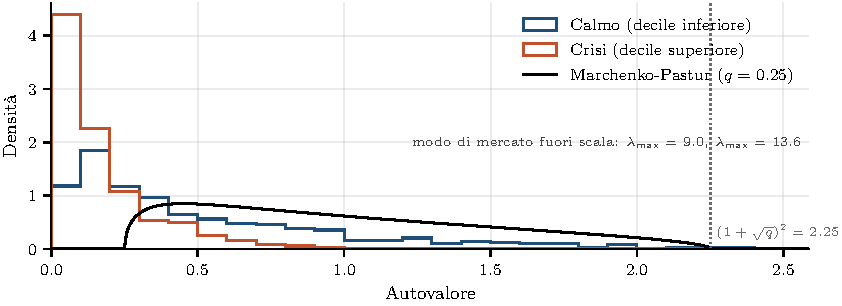
\includegraphics[width=\textwidth]{figures/fig_mp_spectrum.pdf}
\caption[Spettro empirico e legge di Marchenko--Pastur]{Autovalori delle matrici di correlazione nei decili di finestre con la correlazione media più bassa e più alta, confrontati con la densità di Marchenko--Pastur per $q=0{,}250$. In nessuno dei due regimi lo spettro empirico riempie il bulk.}
\label{fig:topo-mp-spectrum}
\end{figure}

\section{Sintesi delle metriche}
\label{sec:topo-orchestration}

Lo script \path{03_topology_analysis.py} applica le funzioni delle sezioni precedenti a tutte le $1947$ finestre e raccoglie i risultati in un unico DataFrame, con una riga per finestra, indicizzata dalla data di chiusura, e una colonna per metrica. La lunghezza dell'MST è calcolata sulle distanze di Mantegna, le due connettività algebriche su $W_{\mathrm{full}}$, connesso in ogni finestra, e la correlazione media e le tre metriche spettrali direttamente su $C_t$. La densità è l'unica calcolata su un grafo filtrato, perché è l'unica che dipende dalla soglia per definizione, ed è riportata, oltre che alla soglia calibrata $\tau$, alla soglia $\tau_{\mathrm{FWER}}=0{,}4311$, più selettiva perché controlla l'errore sull'insieme delle $105$ coppie, e alla soglia fissa $\tau_{\mathrm{fixed}}=0{,}30$. Le due varianti più rade servono a stabilire se un'eventuale serie piatta sia una proprietà del mercato o della soglia.

\begin{table}[H]
\centering
\caption[Metriche topologiche sull'intero periodo]{Statistiche delle metriche topologiche sulle $1947$ finestre mobili.}
\label{tab:topo-summary}
\small
\begin{tabular}{@{}lrrrrr@{}}
\toprule
\textbf{Metrica} & \textbf{Media} & \textbf{Dev. std} & \textbf{Min} & \textbf{Mediana} & \textbf{Max} \\
\midrule
Correlazione media & $0{,}675$ & $0{,}104$ & $0{,}372$ & $0{,}689$ & $0{,}900$ \\
Densità ($\tau$ calibrata) & $0{,}974$ & $0{,}053$ & $0{,}733$ & $1{,}000$ & $1{,}000$ \\
Densità ($\tau_{\mathrm{FWER}}$) & $0{,}887$ & $0{,}129$ & $0{,}371$ & $0{,}924$ & $1{,}000$ \\
Densità ($\tau_{\mathrm{fixed}}$) & $0{,}950$ & $0{,}079$ & $0{,}562$ & $0{,}990$ & $1{,}000$ \\
Connettività algebrica normalizzata & $1{,}024$ & $0{,}022$ & $0{,}923$ & $1{,}028$ & $1{,}058$ \\
Connettività algebrica combinatoria & $7{,}046$ & $1{,}252$ & $3{,}750$ & $7{,}060$ & $10{,}443$ \\
Lunghezza MST normalizzata & $0{,}590$ & $0{,}099$ & $0{,}331$ & $0{,}584$ & $0{,}883$ \\
Entropia spettrale & $1{,}242$ & $0{,}282$ & $0{,}518$ & $1{,}221$ & $2{,}003$ \\
Quota del modo di mercato & $0{,}711$ & $0{,}091$ & $0{,}449$ & $0{,}724$ & $0{,}907$ \\
Autovalori fuori dal bulk & $1{,}004$ & $0{,}064$ & $1{,}000$ & $1{,}000$ & $2{,}000$ \\
\bottomrule
\end{tabular}
\end{table}

Non tutte le serie della \cref{tab:topo-summary} portano lo stesso segnale. La densità alla soglia calibrata ha media $0{,}974$ e mediana $1{,}000$. In più di metà delle finestre nessun arco viene rimosso e il grafo filtrato coincide con quello completo. Alla soglia $\tau_{\mathrm{FWER}}$ la serie varia molto di più (deviazione standard $0{,}129$ contro $0{,}053$). La piattezza è quindi in buona parte un effetto della soglia calibrata, che su un mercato così correlato lascia passare quasi ogni arco.

Le due connettività algebriche si comportano in modo molto diverso. Quella normalizzata resta nell'intervallo $[0{,}923;\,1{,}058]$, con un coefficiente di variazione di $0{,}021$. Quella combinatoria si estende da $3{,}750$ a $10{,}443$, con un coefficiente di variazione di $0{,}178$. La seconda, per questo motivo, compare tra le metriche principali lette attorno alle crisi nella \cref{sec:topo-event-study}.

L'entropia spettrale non supera mai $2{,}003$, ben al di sotto del massimo teorico $\log 15\approx2{,}708$. Una struttura comune ai quindici asset non scompare mai del tutto, nemmeno nella finestra più tranquilla. La quota del modo di mercato quantifica questa struttura. In media il $71\%$ della varianza totale è spiegato dalla sola direzione in cui tutti gli asset si muovono insieme.

Il conteggio degli autovalori fuori dal bulk vale esattamente $1$ in $1939$ finestre su $1947$ e non supera mai $2$. È un risultato distributivo che conferma sui dati dello studio quello di \textcite{laloux1999noise}. Solo il modo di mercato eccede in modo sistematico ciò che il rumore di stima potrebbe produrre da solo.

\section{Il grafo attorno alle crisi}
\label{sec:topo-event-study}

Il periodo di studio include le tre crisi presentate nell'Introduzione: la stretta cinese su scambi e mining del 19/05/2021~\cite{griffith2023cryptocurrency}, il collasso di Terra/Luna del 09/05/2022~\cite{briola2023anatomy} e il fallimento di FTX dell'08/11/2022~\cite{akyildirim2023understanding}. Occorre stabilire se le serie della \cref{sec:topo-orchestration} si muovano in corrispondenza di questi eventi, e con quale intensità rispetto all'intera storia del campione.

\subsection{Offset e percentili}

Il valore alla data $t$ è calcolato sulla finestra di rendimenti $[t-59,\,t]$, quindi alla data dell'evento la finestra termina con il giorno dello shock e i restanti cinquantanove giorni sono tutti precedenti. Lo studio legge perciò ogni metrica a cinque offset dalla data dell'evento, $-60$, $-30$, $0$, $+30$ e $+60$ giorni. L'offset $+60$ è l'unico la cui finestra è interamente successiva all'evento: all'offset $+30$, infatti, la finestra contiene ancora trenta giorni precedenti, cioè metà dei dati. La lettura ai cinque offset è implementata da \texttt{event\_study} in \path{src/cryptognn/events.py}.

\begin{listing}[H]
\begin{minted}{python}
def event_study(
    topology: pd.DataFrame,
    events: list[Event],
    offsets: tuple[int, ...] = DEFAULT_OFFSETS,
) -> pd.DataFrame:
    # Sanity checks on events and offsets, setup of the records list
    ...
    for event in events:
        event_date = pd.Timestamp(event.date)
        for offset in offsets:
            target = event_date + pd.Timedelta(days=offset)
            date_used, values = _read_at(topology, index, target)
            for metric in topology.columns:
                value = values[metric] if values is not None else np.nan
                records.append(
                    {
                        # Event and metric identifiers
                        ...
                        "offset_days": offset,
                        "value": value,
                        "percentile": _percentile(topology[metric], value),
                    }
                )
    study = pd.DataFrame.from_records(records)
    outer = _change_between(study, offsets[0], offsets[-1])
    inner = _change_between(study, offsets[1], offsets[-2]) if len(offsets) >= 4 else pd.Series(np.nan, index=outer.index)
    study["pct_change_clean"] = _broadcast(study, outer)
    study["pct_change_local"] = _broadcast(study, inner)
    return study
\end{minted}
\caption{\texttt{event\_study}}
\label{lst:event-study}
\end{listing}

Il ciclo principale produce una riga per ogni combinazione di evento, offset e metrica. Ogni riga riporta il valore letto e il suo percentile, cioè la frazione dell'intero campione di $1947$ finestre strettamente inferiore a quel valore. Il percentile rende confrontabili metriche su scale diverse. La correlazione media vive in $[0,1]$, la connettività combinatoria tra $3{,}75$ e $10{,}44$, ma un valore al $99$\textdegree{} percentile ha lo stesso significato per entrambe. Un offset che cade fuori dal campione restituisce un valore mancante invece della data disponibile più vicina, che potrebbe distare mesi. A valle del ciclo, le variazioni percentuali sono calcolate da \texttt{\_change\_between}.

\begin{listing}[H]
\begin{minted}{python}
def _change_between(study: pd.DataFrame, start_offset: int, end_offset: int) -> pd.Series:
    pivot = study.pivot_table(
        index=["event_key", "metric"], columns="offset_days", values="value", dropna=False
    )
    return 100.0 * (pivot[end_offset] - pivot[start_offset]) / pivot[start_offset]
\end{minted}
\caption{\texttt{\_change\_between}}
\label{lst:change-between}
\end{listing}

La tabella pivot riorganizza le righe prodotte dal ciclo, con una riga per ogni coppia di evento e metrica e una colonna per ogni offset. L'istruzione \texttt{return} calcola, per ogni coppia, la variazione percentuale del valore $x$ della metrica tra due offset $a$ e $b$:
\begin{equation}
    \Delta_{a\to b} = 100\cdot\frac{x_b-x_a}{x_a}.
    \label{eq:pct-change}
\end{equation}
La variazione principale, $\Delta_{-60\to+60}$, confronta la finestra interamente precedente all'evento con quella interamente successiva. La secondaria, $\Delta_{-30\to+30}$, è tra gli offset interni ed è definita solo quando gli offset sono almeno quattro.

\subsection{Risultati}

La \Cref{tab:topo-event-china} riporta le metriche attorno alla stretta cinese a $-60$, $0$ e $+60$ giorni, con la variazione $\Delta_{-60\to+60}$ e il percentile a $+60$ giorni.

\begin{table}[H]
\centering
\caption[Metriche attorno alla stretta cinese]{Metriche topologiche attorno alla stretta cinese (19/05/2021)~\cite{griffith2023cryptocurrency}. La colonna \%+60g riporta il percentile a $+60$ giorni.}
\label{tab:topo-event-china}
\begin{tabular*}{\textwidth}{@{\extracolsep{\fill}}lrrrrr@{}}
\toprule
\textbf{Metrica} & \textbf{$\mathbf{-60}$g} & \textbf{0g} & \textbf{+60g} & $\mathbf{\Delta_{-60\to+60}}$ & \textbf{\%+60g} \\
\midrule
Corr. media & $0{,}430$ & $0{,}611$ & $0{,}868$ & $+101{,}8\%$ & $99{,}4\%$ \\
Densità ($\tau$) & $0{,}848$ & $0{,}971$ & $1{,}000$ & $+18{,}0\%$ & $36{,}0\%$ \\
Densità ($\tau_{\mathrm{FWER}}$) & $0{,}438$ & $0{,}790$ & $1{,}000$ & $+128{,}3\%$ & $72{,}9\%$ \\
Connett. comb. & $5{,}284$ & $6{,}254$ & $9{,}848$ & $+86{,}4\%$ & $99{,}3\%$ \\
Lunghezza MST & $0{,}826$ & $0{,}654$ & $0{,}386$ & $-53{,}3\%$ & $0{,}5\%$ \\
Entropia spettrale & $1{,}873$ & $1{,}418$ & $0{,}652$ & $-65{,}2\%$ & $0{,}5\%$ \\
Modo di mercato & $0{,}499$ & $0{,}658$ & $0{,}878$ & $+76{,}0\%$ & $99{,}4\%$ \\
\bottomrule
\end{tabular*}
\end{table}

La \Cref{tab:topo-event-china} omette la densità a soglia fissa $\tau_{\mathrm{fixed}}$, ridondante con le altre due, la connettività normalizzata perché pressoché piatta e il conteggio degli autovalori fuori dal bulk, che vale $1$ ad ogni offset. Il valore $1{,}000$ è il massimo possibile per la densità a $+60$ giorni, ma il percentile conta solamente le finestre con valore strettamente inferiore. Poiché il $64\%$ delle finestre ha densità esattamente pari a $1$, un grafo saturo si colloca al $36$\textdegree{} percentile.

La stretta cinese rappresenta il caso caratteristico del compattamento descritto nella \cref{sec:topo-measuring-compaction}: la correlazione media raddoppia tra le due finestre disgiunte, la connettività combinatoria sale dell'$86{,}4\%$ e la quota del modo di mercato del $76{,}0\%$. Ogni metrica si muove nella direzione attesa e quasi ognuna raggiunge un estremo della propria distribuzione storica. La \cref{fig:topo-china} ritrae la finestra a $+60$ giorni. Alla soglia calibrata il grafo è completo, compattamento osservabile nello spessore degli archi e nella matrice di correlazione.

\begin{figure}[H]
\centering
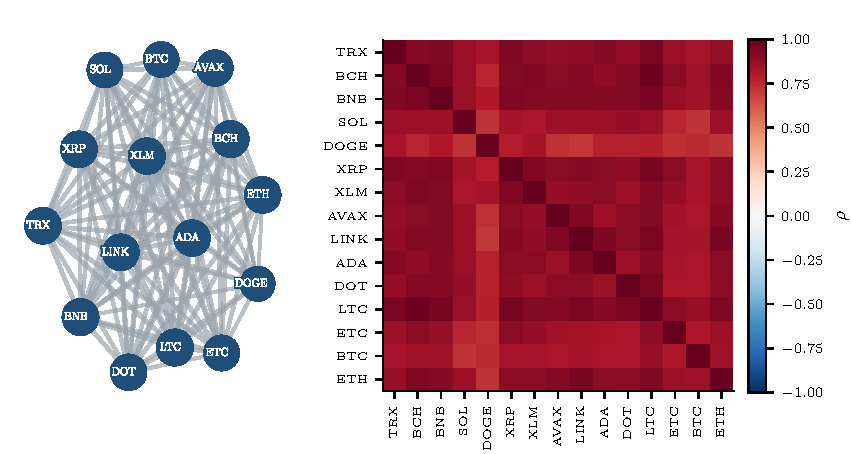
\includegraphics[width=\textwidth]{figures/fig_event_china_crackdown.pdf}
\caption[Grafo e correlazioni a $+60$ giorni dalla stretta cinese]{Finestra a $+60$ giorni dalla stretta cinese (18/07/2021). A sinistra il grafo filtrato $W_{\mathrm{thresh}}$, con lo spessore di ogni arco proporzionale al peso e la dimensione di ogni nodo al grado pesato; le posizioni dei nodi sono calcolate una sola volta sul grafo medio dell'intero periodo e riusate in tutte e tre le figure di evento. A destra la matrice di correlazione $C_t$ della stessa finestra, con gli asset ordinati per clustering gerarchico e la scala del colore fissata a $[-1,1]$.}
\label{fig:topo-china}
\end{figure}

\begin{table}[H]
\centering
\caption[Metriche attorno a Terra/Luna e FTX]{Variazione $\Delta_{-60\to+60}$ e percentile a $+60$ giorni per Terra/Luna (09/05/2022)~\cite{briola2023anatomy} e FTX (08/11/2022)~\cite{akyildirim2023understanding}.}
\label{tab:topo-event-terra-ftx}
\begin{tabular*}{\textwidth}{@{\extracolsep{\fill}}lrrrr@{}}
\toprule
 & \multicolumn{2}{c}{\textbf{Terra/Luna}} & \multicolumn{2}{c}{\textbf{FTX}} \\
\cmidrule(lr){2-3}\cmidrule(lr){4-5}
\textbf{Metrica} & $\mathbf{\Delta_{-60\to+60}}$ & \textbf{\%+60g} & $\mathbf{\Delta_{-60\to+60}}$ & \textbf{\%+60g} \\
\midrule
Corr. media & $-1{,}1\%$ & $86{,}7\%$ & $+7{,}0\%$ & $91{,}6\%$ \\
Densità ($\tau$) & $0{,}0\%$ & $36{,}0\%$ & $0{,}0\%$ & $36{,}0\%$ \\
Densità ($\tau_{\mathrm{FWER}}$) & $-1{,}9\%$ & $62{,}5\%$ & $0{,}0\%$ & $72{,}9\%$ \\
Connett. comb. & $-20{,}2\%$ & $64{,}7\%$ & $+6{,}1\%$ & $95{,}5\%$ \\
Lunghezza MST & $-1{,}8\%$ & $14{,}6\%$ & $-15{,}9\%$ & $13{,}0\%$ \\
Entropia spettrale & $-2{,}9\%$ & $12{,}2\%$ & $-17{,}8\%$ & $11{,}5\%$ \\
Modo di mercato & $-0{,}3\%$ & $87{,}1\%$ & $+6{,}5\%$ & $90{,}2\%$ \\
\bottomrule
\end{tabular*}
\end{table}

Le due crisi del 2022 presentano un quadro diverso (\cref{tab:topo-event-terra-ftx}). La densità alla soglia calibrata vale $1{,}000$ a tutti e cinque gli offset, per entrambi gli eventi. Il grafo filtrato era quindi già completo prima dello shock e non aveva margine per compattarsi ulteriormente. Le variazioni delle altre metriche sono contenute. Per FTX vanno tutte nella direzione del compattamento, con ampiezze tra il $6\%$ e il $18\%$. Per Terra/Luna i segni sono misti e la connettività combinatoria scende del $20{,}2\%$. I percentili forniscono però un'importante lettura. A $+60$ giorni da entrambi gli eventi la correlazione media e la quota del modo di mercato si collocano sopra l'$85$\textdegree{} percentile, l'entropia spettrale e la lunghezza dell'MST sotto il $15$\textdegree{}. Il mercato si trovava in uno stato di forte compattamento, anche prima degli eventi. A $-60$ giorni la correlazione media valeva $0{,}799$ per Terra/Luna e $0{,}753$ per FTX, contro una media storica di $0{,}675$. Nel 2022 la struttura del mercato era quindi già vicina alla saturazione, e una crisi può spostare di poco metriche che si trovano già vicino al proprio estremo. Le \cref{fig:topo-terra-luna,fig:topo-ftx} ritraggono le finestre a $+60$ giorni dei due eventi: grafi completi come quello della stretta cinese e matrici sature nella stessa misura, a dodici e a diciotto mesi di distanza.

\begin{figure}[H]
\centering
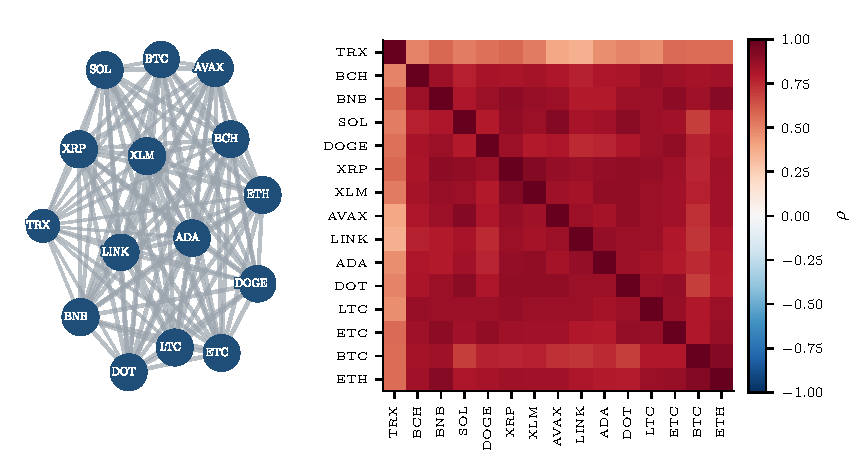
\includegraphics[width=\textwidth]{figures/fig_event_terra_luna.pdf}
\caption[Grafo e correlazioni a $+60$ giorni da Terra/Luna]{Finestra a $+60$ giorni dal collasso di Terra/Luna (08/07/2022), disegnata come la \cref{fig:topo-china}: grafo filtrato a sinistra, matrice di correlazione a destra, stesse posizioni dei nodi e stesso ordinamento degli asset.}
\label{fig:topo-terra-luna}
\end{figure}

\begin{figure}[H]
\centering
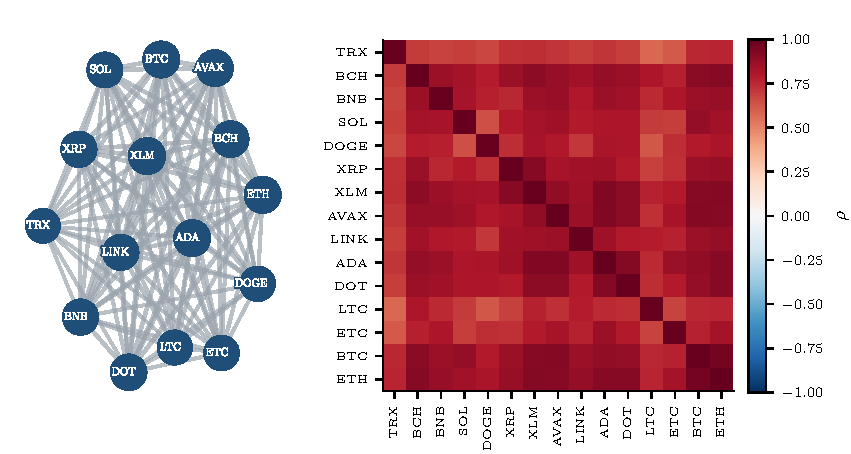
\includegraphics[width=\textwidth]{figures/fig_event_ftx.pdf}
\caption[Grafo e correlazioni a $+60$ giorni dal fallimento di FTX]{Finestra a $+60$ giorni dal fallimento di FTX (07/01/2023), disegnata come la \cref{fig:topo-china}.}
\label{fig:topo-ftx}
\end{figure}

La \Cref{fig:topo-timeseries} riassume l'intero periodo, con quattro delle serie sulle $1947$ finestre e le tre date di crisi sovrapposte. L'asse temporale è condiviso, così che la linea verticale di un evento si legga su tutti i pannelli contemporaneamente. Dopo la stretta cinese ogni pannello mostra un salto netto, mentre le linee di Terra/Luna e FTX cadono su serie già vicine ai propri estremi.

\begin{figure}[H]
\centering
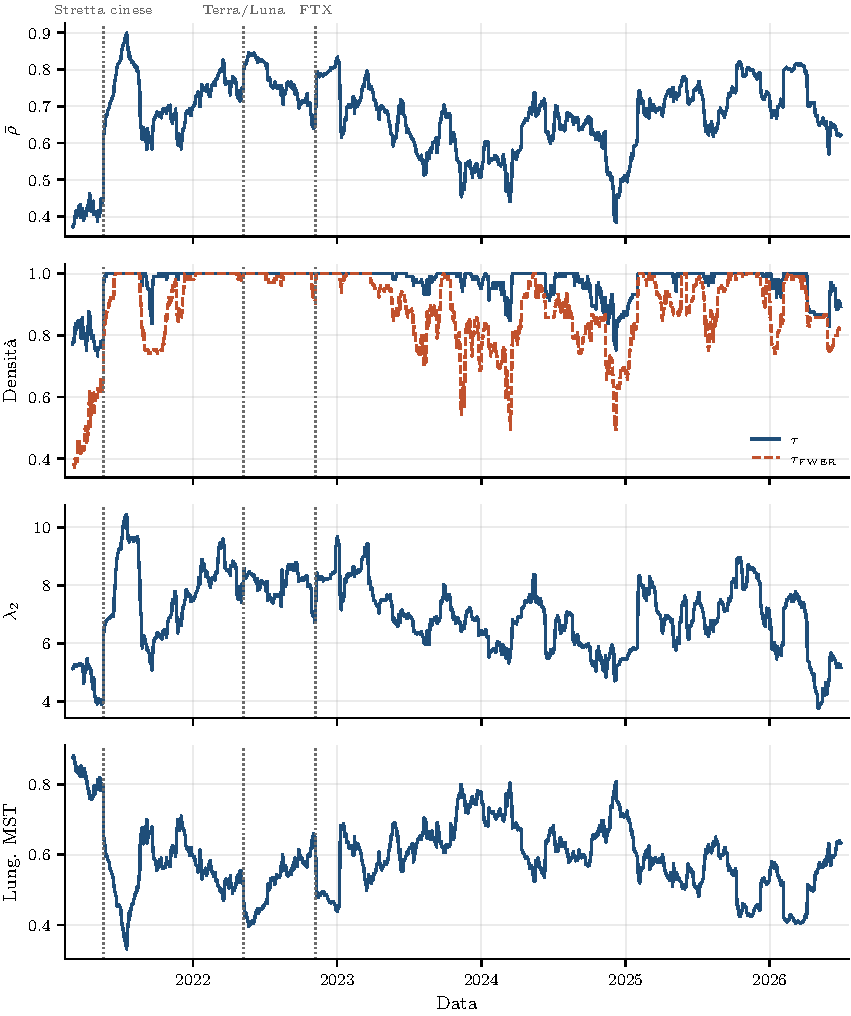
\includegraphics[width=\textwidth]{figures/fig_topology_timeseries.pdf}
\caption[Serie temporali delle metriche topologiche]{Correlazione media, densità alle soglie $\tau$ e $\tau_{\mathrm{FWER}}$, connettività algebrica combinatoria e lunghezza normalizzata dell'MST sulle $1947$ finestre dell'intero periodo, con le date dei tre eventi di crisi sovrapposte a ogni pannello.}
\label{fig:topo-timeseries}
\end{figure}

\chapter{Addestramento e confronto dei modelli}
\label{ch:training-and-comparison}

Il \Cref{ch:forecasting-models} ha definito la GCN e le baseline con cui confrontarne le prestazioni da un punto di vista prettamente teorico, senza stabilire come ogni modello venga addestrato o come le sue previsioni siano giudicate. Questo capitolo sviluppa il protocollo \emph{walk-forward} di addestramento e validazione e i test di significatività statistica sui confronti tra modelli.

\section{Insidie della validazione}
\label{sec:tc-pitfalls}

La pipeline del caso di studio seleziona la procedura di \emph{training} evitando errori metodologici che falserebbero le prestazioni della stima. L'errore misurato sul blocco di test è una stima di quello che il modello commetterebbe in un impiego reale, distorta verso l'ottimismo ogni volta che il protocollo concede al modello informazioni che in quell'impiego non avrebbe. Sui rendimenti finanziari, dove il rapporto segnale-rumore è basso, questa distorsione può superare in ampiezza il segnale stesso. Si distinguono le seguenti insidie ricorrenti.

\subsection{Look-ahead bias}

Consiste nell'usare informazione non ancora disponibile alla chiusura del giorno $t$ per prevedere $r_{t+1}$. Si verifica anche in operazioni come la standardizzazione delle feature: calcolare media e deviazione standard sull'intero campione, addestramento e test insieme, inietta nel modello informazioni sulla distribuzione futura dei dati. La pipeline non fallisce, ma i risultati migliorano in modo silenzioso.

\subsection{Data snooping}

Si realizza quando gli stessi dati sono usati sia per scegliere che per valutare un modello. È probabile che, tra molte configurazioni prive di capacità predittiva provate sullo stesso blocco di test, almeno una batta il riferimento per puro caso: il suo vantaggio è un effetto della selezione e cresce con il numero di configurazioni provate. Il \enquote{Reality Check} di \textcite{white2000reality} ne tiene conto confrontando il modello migliore non con il riferimento, ma con il miglior risultato che l'insieme dei modelli provati otterrebbe per caso. La pipeline di progetto impedisce il \emph{data snooping} fissando in anticipo la griglia della GCN (\cref{sec:tc-gcn-training}) e correggendo i test multipli del confronto finale con il metodo di Holm (\cref{sec:tc-significance}).

\subsection{Validazione incrociata su serie temporali}

La $k$-fold \emph{cross-validation} suddivide i dati in $k$ blocchi, addestrando il modello $k$ volte, ciascuna su $k-1$ blocchi, e valutandolo su quello escluso. Su una serie temporale, il modello viene addestrato anche su osservazioni successive a quelle su cui è valutato, violando l'ordine temporale che incontrerebbe in un impiego reale.

\section{Il protocollo walk-forward}
\label{sec:tc-walkforward}

La validazione walk-forward ovvia al problema della $k$-fold rispettando l'ordine temporale dei dati. Il modello viene addestrato su una finestra di osservazioni e valutato sul periodo immediatamente successivo. La finestra avanza rispetto all'inizio della precedente, ripetendo poi la procedura. Ogni valutazione avviene quindi su dati posteriori a quelli di training. Nello studio, il modello si colloca alla chiusura del giorno $t$ e prevede $r_{t+1}$ utilizzando le sole osservazioni fino a $t$ compreso.

\subsection{La finestra causale}

Per evitare che, all'origine $t$, il modello includa anche la riga $t+1$, il rendimento da prevedere, ogni input dei modelli è estratto da \texttt{causal\_windows}. Questa funzione si occupa di aggiungere, in testa al pannello, $\texttt{window}-1$ righe di \texttt{NaN} e di ricavare, con \texttt{sliding\_window\_view}, tutte le finestre consecutive. A partire da un pannello $(T, N)$, come quello dei rendimenti $r\in\mathbb{R}^{2006\times 15}$ ricavato alla \cref{sec:returns-stationarity}, si ottiene un tensore $(T, \texttt{window}, N)$.

\begin{listing}[H]
\begin{minted}{python}
def causal_windows(values: np.ndarray, window: int) -> np.ndarray:
    if values.ndim != 2:
        raise ValueError(f"Expected a (T, N) panel, got {values.ndim} dimensions")
    if window < 1:
        raise ValueError(f"Window must be at least 1, got {window}")
    if window > len(values):
        raise ValueError(f"Window of {window} exceeds the {len(values)} rows available")

    pad = np.full((window - 1, values.shape[1]), np.nan)
    padded = np.vstack([pad, values])
    return sliding_window_view(padded, window, axis=0).transpose(0, 2, 1)
\end{minted}
\caption{\texttt{causal\_windows}}
\label{lst:causal-windows}
\end{listing}

Per ogni riga $t$ il risultato contiene le \texttt{window} righe che terminano in $t$, in ordine cronologico: \texttt{result[t, -1]} è la riga $t$ stessa e \texttt{result[t, -1 - k]} la riga $t-k$. Le prime righe del risultato, prive di una storia completa, contengono \texttt{NaN}.

\subsection{Le feature dei nodi}
\label{sec:tc-node-features}

Le finestre causali trovano il loro primo utilizzo nel calcolo delle $F=8$ feature, dette anche canali, che la GCN riceve in ingresso per ciascun nodo e ciascuna origine $t$. Sono ricavate dai pannelli dei rendimenti e dei volumi (\cref{sec:returns-stationarity}) e descrivono tre aspetti diversi del comportamento recente di un asset: il suo andamento, il suo rischio e l'attività di scambio. Fissata l'origine, esse formano la matrice $H^{(0)}\in\mathbb{R}^{N\times F}$ \eqref{eq:gcn}, con una riga per ciascuno dei $15$ asset e una colonna per canale.

I primi cinque canali sono i rendimenti ritardati $r_t, r_{t-1}, \dots, r_{t-4}$. Rappresentano la dinamica di breve periodo del prezzo. Il rendimento $r_t$ è incluso perché noto alla chiusura del giorno in cui si prevede. Il sesto e il settimo canale sono la volatilità realizzata su $5$ e $20$ giorni, cioè l'ampiezza tipica dei rendimenti recenti. Rappresentano il livello di rischio corrente dell'asset e riflettono il volatility clustering (\cref{sec:stylized-facts}). L'ottavo canale confronta il logaritmo del volume scambiato nel giorno $t$ con la sua media sugli ultimi $20$ giorni, $t$ compreso, espresso in deviazioni standard. Un volume insolitamente alto segnala in genere l'arrivo di nuova informazione o un cambiamento nell'interesse degli operatori, e accompagna spesso i movimenti di prezzo più ampi. Prima di essere usate nella GCN, le feature sono standardizzate separatamente in ciascun fold (\cref{sec:tc-single-training}).

\subsection{La geometria dei fold}

Lo studio usa uno schema walk-forward di tipo \emph{rolling} con $24$ fold. I fold vengono ricavati direttamente dal pannello dei rendimenti $r$ (\cref{sec:returns-stationarity}): ognuno di essi è costituito da un training set di $365$ \emph{entry}, un validation set di $63$ entry ed un test set di $63$ entry. Il fold successivo ha inizio $63$ righe dopo l'inizio del precedente: l'addestramento mantiene in questo modo una lunghezza fissa e i blocchi di test di fold consecutivi si affiancano senza sovrapporsi.

Il primo fold parte dalla posizione $T_w-1=59$, perché prima della sessantesima osservazione non esiste alcun grafo di correlazione (\cref{sec:correlation-matrix-to-graph}). I fold vengono aggiunti fino a quando il successivo non supera l'ultima riga utilizzabile per prevedere $r_{t+1}$, ovvero la penultima riga del pannello. Il periodo di test va dal 05/05/2022 al 24/06/2026, per $1512$ giorni e $22\,680$ previsioni per modello sui $15$ asset.

Ogni fold, al momento della sua costruzione, verifica che i tre insiemi siano non vuoti, formati da righe consecutive del pannello e disposti nell'ordine training, validation, test; in caso contrario l'esecuzione si interrompe con un errore.

\begin{figure}[H]
\centering
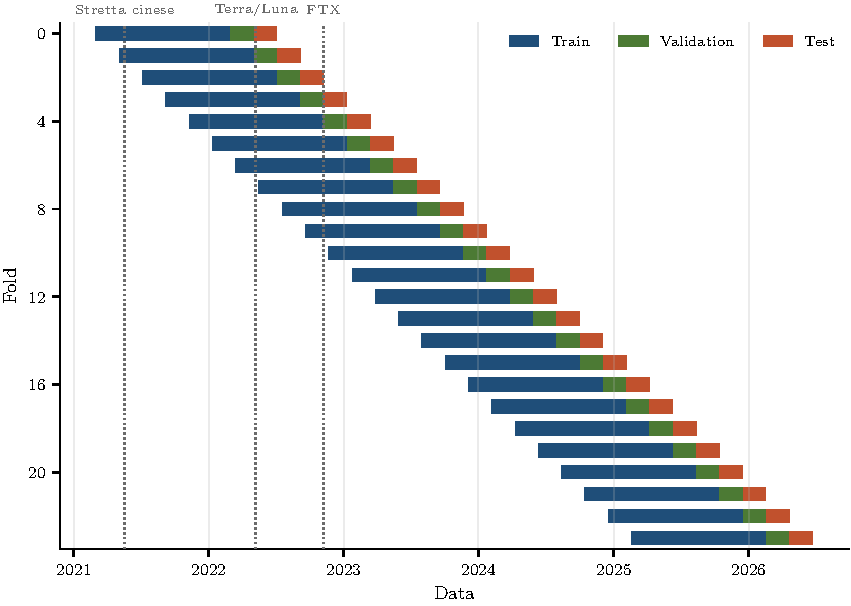
\includegraphics[width=\textwidth]{figures/fig_walkforward_scheme.pdf}
\caption[Schema del protocollo walk-forward]{I $24$ fold del protocollo walk-forward, con addestramento, validazione e test e le date dei tre eventi di crisi. La stretta cinese del 19/05/2021 precede il periodo previsto e compare solo nell'analisi topologica della \cref{sec:topo-event-study}; Terra/Luna e FTX cadono dentro un blocco di test e sono valutate fuori campione.}
\label{fig:tc-walkforward-scheme}
\end{figure}

\subsection{Target del test set}

I modelli utilizzati nello studio (\cref{ch:forecasting-models}) ricevono, per ciascun fold, tre oggetti \texttt{Segment}, uno per blocco (train, validation, test), con le sole righe del blocco corrispondente. La riga $i$ di un segmento contiene rendimenti, feature e adiacenza $\hat A$ all'origine $t_i$, il target $y_i=r_{t_i+1}$ e i ritardi più recenti fino a $t_i$ compreso, ricavati da \texttt{causal\_windows}. I ritardi sono distinti dalle feature: sono i rendimenti nelle loro unità originali, senza standardizzazione, e costituiscono l'ingresso delle baseline autoregressive, che stimano i propri coefficienti direttamente su questi ultimi. Nel blocco di test il target non deve essere accessibile al modello: il metodo \texttt{without\_target} è utilizzato a tal proposito.

\begin{listing}[H]
\begin{minted}{python}
def without_target(self) -> Segment:
    return replace(self, y=np.full_like(self.y, np.nan))
\end{minted}
\caption{\texttt{without\_target}}
\label{lst:without-target}
\end{listing}

Esso restituisce una copia del segmento in cui \texttt{y} è sostituito da \texttt{NaN}. Si impedisce quindi il \emph{data leakage}.

\subsection{Il ciclo di valutazione}

Ogni modello del progetto implementa \texttt{fit(train, val)} e \texttt{predict(segment)}. I modelli che non utilizzano la validazione ricevono comunque \texttt{val} e lo ignorano. Questa firma unica permette a \texttt{run\_walkforward} (\cref{lst:run-walkforward}) di trattare tutti i modelli con lo stesso codice.

Per ciascun fold, \texttt{run\_walkforward} costruisce i tre oggetti \texttt{Segment} e interrompe l'esecuzione se uno di essi contiene feature o adiacenze non finite, segno di un fold che risale a posizioni prive di grafo. Crea poi un modello nuovo tramite \texttt{factory} per ogni fold, affinché i parametri stimati per quello precedente non vengano riutilizzati nel successivo. Il modello viene addestrato su \texttt{train\_segment} e \texttt{val\_segment}, e prevede su \texttt{test\_segment.without\_target()}.

La funzione restituisce un oggetto \texttt{WalkforwardResult}, composto da due tabelle. La prima, \texttt{predictions}, raccoglie le previsioni del solo blocco di test in formato lungo: una riga per fold, data, asset e modello, con il rendimento realizzato \texttt{y\_true} e quello previsto \texttt{y\_pred}. La seconda, \texttt{diagnostics}, contiene una riga per fold con le dimensioni dei tre blocchi e il tempo di addestramento.

\begin{longlisting}{\texttt{run\_walkforward}}{lst:run-walkforward}
\begin{minted}{python}
def run_walkforward(factory: Callable[[], Forecaster], data: WalkforwardData, folds: list[Fold], name: str | None = None, verbose: bool = True) -> WalkforwardResult:

    predictions: list[pd.DataFrame] = []
    diagnostics: list[dict[str, object]] = []
    n_assets = data.n_assets
    assets = np.asarray(data.assets)

    for fold in folds:
        _validate_fold(data, fold)
        train_segment = data.segment(fold.train)
        val_segment = data.segment(fold.val)
        test_segment = data.segment(fold.test)
        for segment, split in ((train_segment, "train"), (val_segment, "val"), (test_segment, "test")):
            _check_finite(segment, fold, split)

        model = factory()
        model_name = name if name is not None else getattr(model, "name", type(model).__name__)

        started = time.perf_counter()
        model.fit(train_segment, val_segment)
        fit_seconds = time.perf_counter() - started

        predicted = np.asarray(model.predict(test_segment.without_target()), dtype=float)
        if predicted.shape != (len(test_segment), n_assets):
            raise ValueError(
                f"Fold {fold.index}: {model_name} predicted {predicted.shape}, "
                f"expected {(len(test_segment), n_assets)}"
            )
        if not np.isfinite(predicted).all():
            raise ValueError(f"Fold {fold.index}: {model_name} produced non-finite predictions")

        predictions.append(
            pd.DataFrame(
                {
                    "fold": fold.index,
                    "date": test_segment.target_dates.repeat(n_assets),
                    "asset": np.tile(assets, len(test_segment)),
                    "y_true": test_segment.y.ravel(),
                    "y_pred": predicted.ravel(),
                    "model": model_name,
                }
            )
        )

        n_train, n_val, n_test = fold.sizes
        row: dict[str, object] = {
            "fold": fold.index,
            "model": model_name,
            "n_train": n_train,
            "n_val": n_val,
            "n_test": n_test,
            "fit_seconds": fit_seconds,
        }
        if isinstance(model, SupportsDiagnostics):
            row.update(model.diagnostics())
        diagnostics.append(row)

        if verbose:
            # Print the fold's block sizes, test dates and fit time.
            ...

    return WalkforwardResult(
        predictions=pd.concat(predictions, ignore_index=True),
        diagnostics=pd.DataFrame(diagnostics),
    )
\end{minted}
\end{longlisting}

Le previsioni delle baseline sono salvate su disco prima dell'addestramento della GCN e successivamente rilette senza essere ricalcolate. Il termine di confronto è in questo modo fissato prima che sia noto il risultato del modello da valutare.

L'assenza di look-ahead (\cref{sec:tc-pitfalls}) è verificata da test dedicati. Si controllano, in particolare, l'ordine dei blocchi di ciascun fold, l'allineamento del grafo, verificando che quello usato per prevedere $r_{t+1}$ sia costruito sui soli rendimenti in $[t-59,t]$, la standardizzazione delle feature (\cref{sec:tc-single-training}) e l'assenza di $r_{t+1}$ in ciascuna di esse. Sui grafi, infatti, la verifica è immediata, poiché è sufficiente dimostrare che $\hat A$ non contenga il rendimento del giorno successivo.

\section{Addestramento della GCN}
\label{sec:tc-gcn-training}

La GCN, a differenza delle baseline del \Cref{ch:forecasting-models}, stimate in forma chiusa o con un criterio di selezione, deve essere addestrata per discesa del gradiente (\cref{sec:from-perceptron-to-graph-layer}): i pesi $W^{(l)}$ e i bias $b^{(l)}$ dell'equazione~\eqref{eq:gcn} sono spostati ripetutamente nella direzione da esso indicata. L'addestramento della rete introduce quindi quattro scelte che le baseline non richiedono: in che forma i dati raggiungono la rete, con quale regola i pesi vengono aggiornati, per quanto a lungo e con quali valori degli iperparametri che il gradiente non tocca. La configurazione è fissata a priori.

\subsection{Gli ingressi della rete}
\label{sec:tc-single-training}

La GCN è l'unico modello dello studio che legge entrambi i tensori dell'oggetto \texttt{Segment}: le feature dei nodi (\cref{sec:tc-node-features}) e le adiacenze $\hat A$ (\cref{sec:correlation-matrix-to-graph}).

Le feature sono standardizzate prima di raggiungere la rete. Media e deviazione standard sono stimate per asset e per canale sul solo blocco di addestramento, e applicate invariate a validazione e test. Stimarle sul solo training evita il look-ahead della \cref{sec:tc-pitfalls}. Stimarle per asset risponde invece alla condivisione dei pesi della \cref{sec:gcn-kipf-welling}: la matrice $W^{(l)}$ è la stessa per tutti i nodi e gli asset differiscono in volatilità fino a un ordine di grandezza.

Il target è invece diviso per un unico scalare $s$, la deviazione standard dei rendimenti di addestramento. I pesi iniziali sono estratti da un intervallo calibrato perché la varianza del segnale si conservi da uno strato al successivo: poiché le feature hanno ormai varianza unitaria, una rete non addestrata restituisce valori di ordine uno, contro rendimenti dell'ordine di $0{,}04$. Senza la divisione, le prime epoche servirebbero solo a ridurre la scala dell'uscita. Lo scalare è unico per l'intero pannello: dividere per una costante moltiplica il costo per $1/s^2$ senza spostarne il minimo. Previsioni ed errori tornano poi in unità di rendimento.

Le adiacenze sono infine allineate al pannello da \texttt{align\_graph}. Il grafo esiste solo dalla sessantesima osservazione (\cref{sec:correlation-matrix-to-graph}), quindi il tensore è più corto di $T_w-1$ righe. Ogni matrice è collocata sulla riga della data in cui la sua finestra si chiude, garantendo che l'adiacenza in posizione $t$ sia costruita sui soli rendimenti fino a $t$. Le righe prive di grafo sono riempite di \texttt{NaN}, non di zeri: un'adiacenza nulla addestrerebbe il modello su un mercato senza relazioni, mentre il \texttt{NaN} si propaga e viene intercettato da \texttt{run\_walkforward} (\cref{sec:tc-walkforward}).

\begin{listing}[H]
\begin{minted}{python}
def align_graph(a_hat: np.ndarray, corr_index: pd.DatetimeIndex, dates: pd.DatetimeIndex) -> np.ndarray:
    # Check the graph tensor and the correlation index have the same length.
    ...
    panel = pd.DatetimeIndex(dates)
    graph_dates = pd.DatetimeIndex(corr_index)
    # Reconcile the timezone of the two indices.
    ...

    positions = panel.get_indexer(graph_dates)
    if (positions < 0).any():
        missing = graph_dates[positions < 0]
        raise ValueError(f"{len(missing)} correlation dates absent from the return panel, first {missing[0]}")

    aligned = np.full((len(dates), *a_hat.shape[1:]), np.nan, dtype=float)
    aligned[positions] = a_hat
    return aligned
\end{minted}
\caption{\texttt{align\_graph}}
\label{lst:align-graph}
\end{listing}

Il tensore restituito ha tante matrici quante sono le righe del pannello, e ciascuna occupa la posizione della propria data di chiusura. Le date del grafo assenti dal pannello ricevono da \texttt{get\_indexer} la posizione $-1$ e interrompono l'esecuzione: le due sorgenti devono descrivere lo stesso periodo perché una posizione $t$ abbia un unico significato.

\subsection{Adam e la regolarizzazione}

Il criterio di aggiornamento dei pesi che la pipeline utilizza è Adam~\cite{kingmaba2015adam}, applicato all'errore quadratico medio (MSE): ogni parametro riceve un passo di dimensione propria, ricavato dalla storia dei suoi gradienti.

Per ciascun parametro $w$ l'ottimizzatore conserva due medie mobili esponenziali, aggiornate a ogni passo $k$ a partire dal gradiente $g_k$ del costo rispetto a $w$
\begin{equation}
\label{eq:adam-moments}
m_k = \beta_1 m_{k-1} + (1-\beta_1)\,g_k, \qquad v_k = \beta_2 v_{k-1} + (1-\beta_2)\,g_k^2.
\end{equation}
La prima memoria, $m_k$, è la media dei gradienti recenti e ne rappresenta la direzione prevalente: se i gradienti di passi successivi concordano, i loro contributi si sommano e il passo accelera; se si alternano di segno, si elidono a vicenda e il passo si accorcia. La seconda, $v_k$, è la media dei loro quadrati e misura l'ampiezza tipica del gradiente di quel parametro, indipendentemente dal segno. I coefficienti $\beta_1$ e $\beta_2$ fissano la lunghezza delle due memorie, ovvero la rapidità con cui il passato viene dimenticato.

Il passo effettivo del parametro si ricava dalle due memorie
\begin{equation}
\label{eq:adam-update}
w_k = w_{k-1} - \eta\,\frac{\hat m_k}{\sqrt{\hat v_k}+\varepsilon}, \qquad \hat m_k = \frac{m_k}{1-\beta_1^k}, \qquad \hat v_k = \frac{v_k}{1-\beta_2^k}.
\end{equation}
Le versioni $\hat m_k$ e $\hat v_k$ correggono le due memorie dalla distorsione dovuta all'inizializzazione a zero, che altrimenti le sottostimerebbe nei primi passi. Dividendo la prima per la radice della seconda si ottiene un passo che non dipende più dalla scala del gradiente, ma soltanto dalla sua costanza; $\varepsilon$ impedisce la divisione per zero; $\eta$ è il passo base, unico per tutti i parametri.

Il vantaggio rispetto alla discesa del gradiente a passo fisso (\cref{sec:from-perceptron-to-graph-layer}) emerge quando una direzione è molto più ripida dell'altra (\cref{fig:tc-adam-vs-gd}). A passo fisso, l'unico $\eta$ disponibile deve essere sufficientemente piccolo da non far divergere la direzione ripida. La traiettoria oscilla allora tra i due versanti della valle, avanzando lentamente lungo il suo fondo. Con Adam, invece, la discesa segue esattamente il fondo della valle.

\begin{figure}[H]
\centering
\begin{subfigure}{\textwidth}
\centering
\begin{tikzpicture}[x=2.0cm, y=2.0cm, every node/.style={font=\small}]
    \foreach \r in {0.75, 1.5, 2.25, 3.0} {
        \draw[gray!45] (0,0) ellipse ({\r} and {\r/3.464});
    }
    \draw[black!70, thick] (-0.45,0) -- (3.15,0);
    \node[font=\scriptsize] at (3.32,0.12) {$w_1$};
    \draw[very thick]
        (2.700,0.450) -- (2.260,-0.430) -- (1.892,0.411) -- (1.583,-0.393) -- (1.325,0.376) --
        (1.109,-0.359) -- (0.928,0.344) -- (0.777,-0.328) -- (0.650,0.314) -- (0.544,-0.300) --
        (0.456,0.287) -- (0.381,-0.274) -- (0.319,0.262) -- (0.267,-0.251) -- (0.224,0.240) --
        (0.187,-0.229) -- (0.157,0.219) -- (0.131,-0.209) -- (0.110,0.200) -- (0.092,-0.191) --
        (0.077,0.183) -- (0.064,-0.175) -- (0.054,0.167) -- (0.045,-0.160) -- (0.038,0.153) --
        (0.032,-0.146) -- (0.026,0.140) -- (0.022,-0.134) -- (0.019,0.128) -- (0.016,-0.122) --
        (0.013,0.117);
    \fill (2.700,0.450) circle (1.3pt);
    \draw[thick] (-0.07,-0.07) -- (0.07,0.07) (-0.07,0.07) -- (0.07,-0.07);
\end{tikzpicture}
\caption{Discesa del gradiente a passo fisso}
\label{fig:tc-adam-vs-gd-a}
\end{subfigure}

\vspace{12pt}

\begin{subfigure}{\textwidth}
\centering
\begin{tikzpicture}[x=2.0cm, y=2.0cm, every node/.style={font=\small}]
    \foreach \r in {0.75, 1.5, 2.25, 3.0} {
        \draw[gray!45] (0,0) ellipse ({\r} and {\r/3.464});
    }
    \draw[black!70, thick] (-0.45,0) -- (3.15,0);
    \node[font=\scriptsize] at (3.32,0.12) {$w_1$};
    \draw[very thick]
        (2.700,0.450) -- (2.595,0.345) -- (2.490,0.242) -- (2.385,0.142) -- (2.281,0.048) --
        (2.177,-0.035) -- (2.074,-0.103) -- (1.971,-0.154) -- (1.869,-0.185) -- (1.768,-0.198) --
        (1.668,-0.194) -- (1.569,-0.178) -- (1.472,-0.153) -- (1.376,-0.120) -- (1.281,-0.083) --
        (1.189,-0.044) -- (1.098,-0.006) -- (1.009,0.029) -- (0.923,0.059) -- (0.839,0.082) --
        (0.757,0.097) -- (0.678,0.104) -- (0.602,0.104) -- (0.529,0.096) -- (0.459,0.083) --
        (0.392,0.065) -- (0.329,0.045) -- (0.269,0.023) -- (0.212,0.001) -- (0.159,-0.018) --
        (0.109,-0.035);
    \fill (2.700,0.450) circle (1.3pt);
    \draw[thick] (-0.07,-0.07) -- (0.07,0.07) (-0.07,0.07) -- (0.07,-0.07);
\end{tikzpicture}
\caption{Adam}
\label{fig:tc-adam-vs-gd-b}
\end{subfigure}
\caption[Discesa del gradiente e Adam a confronto]{Trenta passi dei due metodi sulla stessa funzione di costo quadratica $C(w_1,w_2)=\tfrac12\left(w_1^2+12\,w_2^2\right)$, a partire dallo stesso punto. Le ellissi sono le curve di livello di $C$, la croce il suo minimo e il punto la posizione iniziale. La direzione $w_2$ è dodici volte più ripida di $w_1$.}
\label{fig:tc-adam-vs-gd}
\end{figure}

Si applicano due meccanismi per limitare l'adattamento al rumore del blocco di addestramento. Il primo è il \emph{weight decay}, fissato a $0{,}0005$, che ad ogni passo riduce leggermente la norma dei pesi, penalizzando le soluzioni di ampiezza elevata. Il secondo è il \emph{dropout}~\cite{srivastava2014dropout}: durante l'addestramento ciascuna componente del tensore in ingresso ad uno strato è azzerata con probabilità $p$, indipendentemente dalle altre, riscalando le componenti superstiti affinché la somma resti della stessa ampiezza. Nell'architettura a due strati della \cref{sec:known-limitations-gnn}, il dropout è applicato prima di ciascuno dei due ed è attivo soltanto in fase di training: in valutazione, la rete è deterministica e usa tutte le componenti. L'addestramento è \emph{full-batch}. Ogni epoca corrisponde quindi ad un solo passo di Adam, calcolato su tutte le origini del blocco.

\subsection{Epoche ed early stopping}

Il numero di epoche dipende dal singolo fold. Il ciclo di \texttt{fit} ne esegue al più $300$ e affida al blocco di validazione la decisione di fermarsi prima.

\begin{listing}[H]
\begin{minted}{python}
for epoch in range(1, self.epochs + 1):
    model.train()
    optimizer.zero_grad()
    criterion(model(train_a, train_x), train_y).backward()
    optimizer.step()
    in_returns = self.target_scale_**2
    model.eval()
    with torch.no_grad():
        val_mse = float(criterion(model(val_a, val_x), val_y)) * in_returns
    if val_mse < best_val:
        best_val, best_epoch = val_mse, epoch
        best_state = copy.deepcopy(model.state_dict())
        waited = 0
    else:
        waited += 1
        if waited >= self.patience:
            break
model.load_state_dict(best_state)
\end{minted}
\caption{\texttt{fit}}
\label{lst:gcn-fit}
\end{listing}

Dopo ogni passo di ottimizzazione l'errore è ricalcolato in modalità \texttt{eval}, cioè senza dropout, perché la quantità su cui si decide deve essere quella della rete che verrà poi usata per prevedere. Se l'MSE di validazione migliora, i pesi correnti sono copiati e il contatore di attesa azzerato; se non migliora per $30$ epoche consecutive l'addestramento si arresta. Questa procedura prende il nome di \emph{early stopping}.

Senza il ripristino di \texttt{best\_state} il modello conservato sarebbe quello di $30$ epoche successive al minimo, strettamente peggiore del migliore osservato e da esso indistinguibile in qualunque log. I semi casuali, infine, sono fissati all'inizio di \texttt{fit} e non nel costruttore, così che rieseguire un singolo fold riproduca esattamente il risultato che quel fold ha prodotto nell'esecuzione completa.

\subsection{La griglia e la selezione}

Gli iperparametri che intervengono nell'addestramento della GCN e che il gradiente non tocca sono due, e costituiscono una griglia fissata prima di osservare qualunque risultato. Le \emph{hidden units} valgono $16$ o $32$: è la dimensione interna delle due matrici dell'equazione~\eqref{eq:gcn}, cioè la larghezza della rappresentazione $H^{(1)}$, e quindi la capacità del modello. Il dropout vale invece $0{,}2$ o $0{,}5$. La profondità resta fissa a due strati. Fissare la griglia risponde al data snooping della \cref{sec:tc-pitfalls}: il numero di configurazioni provate è dichiarato in anticipo e non cresce dopo aver visto il blocco di test.

Si ottengono quindi quattro configurazioni, ciascuna delle quali è addestrata, per ogni fold, con $5$ semi diversi per la generazione casuale dei pesi iniziali. I semi non aggiungono un terzo asse, perché non si sceglie tra loro: le $5$ reti di una stessa configurazione sono mediate e la previsione della configurazione è la media delle loro previsioni. Il criterio di selezione che ne segue è l'MSE di validazione della media delle $5$ previsioni e non la media dei $5$ MSE. La quantità su cui si sceglie coincide così con quella che il blocco di test misurerà, e la previsione finale del fold è quella della sola configurazione selezionata. Anche le previsioni di validazione, infine, sono richieste su un segmento privato del target, alle stesse condizioni del test. Sui $24$ fold e sui due bracci della \cref{sec:tc-ablation} lo studio addestra quindi $960$ reti.

\begin{table}[H]
\centering
\caption[MSE di validazione sulla griglia GCN]{MSE di validazione medio sui $24$ fold per ciascuna cella della griglia fissata, per i due bracci dell'ablation.}
\label{tab:tc-gcn-grid}
\small
\begin{tabular*}{\textwidth}{@{\extracolsep{\fill}}rrrr@{}}
\toprule
\textbf{Hidden units} & \textbf{Dropout} & \textbf{GCN} & \textbf{GCN senza grafo} \\
\midrule
$16$ & $0{,}2$ & $0{,}001726$ & $0{,}001745$ \\
$16$ & $0{,}5$ & $0{,}001725$ & $0{,}001736$ \\
$32$ & $0{,}2$ & $0{,}001725$ & $0{,}001738$ \\
$32$ & $0{,}5$ & $0{,}001725$ & $0{,}001733$ \\
\bottomrule
\end{tabular*}
\end{table}

\begin{table}[H]
\centering
\caption[Esito della selezione sulla griglia GCN]{Configurazione più spesso selezionata sui $24$ fold, con il suo MSE di validazione, le epoche medie di addestramento e la quota di addestramenti interrotti dall'early stopping.}
\label{tab:tc-gcn-selection}
\small
\begin{tabular*}{\textwidth}{@{\extracolsep{\fill}}lcrrr@{}}
\toprule
\textbf{Braccio} & \textbf{Configurazione} & \textbf{MSE val.} & \textbf{Epoche} & \textbf{Early stop} \\
\midrule
GCN & $h{=}16,\,p{=}0{,}5$ ($9/24$) & $0{,}001706$ & $66{,}7$ & $100{,}0\%$ \\
GCN senza grafo & $h{=}32,\,p{=}0{,}2$ ($9/24$) & $0{,}001720$ & $91{,}8$ & $98{,}3\%$ \\
\bottomrule
\end{tabular*}
\end{table}

Nella \cref{tab:tc-gcn-grid} le quattro celle della GCN coincidono fino alla quinta cifra decimale, e il vantaggio del braccio con grafo su quello senza, pur presente in ogni cella, non supera la dispersione interna alla griglia del braccio senza grafo. La selezione non distingue meglio: i due bracci non convergono sulla stessa configurazione più frequente e ciascuna delle due si aggiudica appena $9$ fold su $24$ (\cref{tab:tc-gcn-selection}), con un MSE che, essendo un minimo scelto fold per fold, non è confrontabile con le medie della tabella precedente. Una griglia così piatta è coerente con l'assenza di un segnale predittivo più che con un'esplorazione insufficiente.

\section{Lo studio di ablation}
\label{sec:tc-ablation}

Confrontare la GCN con le baseline di riferimento non è sufficiente per isolare il contributo del grafo. La rete neurale, infatti, differisce dai modelli autoregressivi anche per le feature di ingresso, per la non linearità e per la procedura di addestramento. Un eventuale vantaggio potrebbe dipendere da uno di questi fattori. Uno studio di ablation rimuove una sola componente del modello, lasciando invariato tutto il resto. Nel progetto, la componente rimossa è l'adiacenza $\hat A$, sostituita con la matrice identità $I$ prima di applicare i due layer.

Con $\hat A=I$ l'equazione~\eqref{eq:gcn} si riduce a $H^{(l+1)}=\sigma\bigl(H^{(l)}W^{(l)}+b^{(l)}\bigr)$, un percettrone applicato a ciascun nodo separatamente con gli stessi pesi. L'unica differenza tra i due bracci riguarda la considerazione delle informazioni dei vicini. I due bracci sono costruiti da \texttt{gcn\_factories}.

\begin{listing}[H]
\begin{minted}{python}
def gcn_factories(config: Config) -> dict[str, Callable[[], GCNGridForecaster]]:
    return {
        name: lambda use_graph=use_graph: GCNGridForecaster(config, use_graph=use_graph)
        for name, use_graph in (("gcn", True), ("gcn-nograph", False))
    }
\end{minted}
\caption{\texttt{gcn\_factories}}
\label{lst:gcn-factories}
\end{listing}

I due bracci sono poi eseguiti, come le baseline, attraverso \texttt{run\_walkforward}. Il confronto tra \texttt{gcn} e \texttt{gcn-nograph} è la forma più diretta della prima questione di ricerca posta nell'Introduzione. Il suo esito è riportato nella \cref{sec:tc-results}.

\section{Lo skill score}
\label{sec:tc-skill-score}

La \cref{sec:baselines} ha osservato che la previsione nulla $\hat r_{t+1,a}=0$ si colloca, sui rendimenti giornalieri, vicino all'errore quadratico medio minimo raggiungibile. L'errore di un modello, preso singolarmente, non fornisce sufficiente informazione. Sul periodo di test dello studio, la previsione nulla ha un RMSE di $0{,}04145$. Si giudicano gli altri modelli rispetto a questo valore. Lo skill score rende esplicito il confronto
\begin{equation}
\label{eq:skill-score}
\mathrm{skill} = 1-\frac{\mathrm{MSE}_{\text{modello}}}{\mathrm{MSE}_{\text{zero}}},
\end{equation}
e rappresenta la frazione dell'errore quadratico della previsione nulla che il modello riesce a muovere. Lo skill score vale $0$ per un modello equivalente alla previsione nulla; è positivo quando il modello la batte e negativo in caso contrario, senza alcun limite inferiore. Il valore massimo $1$ corrisponde ad una previsione perfetta del modello confrontato.

\begin{listing}[H]
\begin{minted}{python}
def skill_score(y: np.ndarray, pred: np.ndarray, baseline_pred: np.ndarray) -> float:
    baseline_mse = float(np.mean((np.asarray(y) - np.asarray(baseline_pred)) ** 2))
    if baseline_mse <= 0:
        raise ValueError("Baseline MSE is zero: the skill score is undefined against a perfect reference")
    return 1.0 - float(np.mean((np.asarray(y) - np.asarray(pred)) ** 2)) / baseline_mse
\end{minted}
\caption{\texttt{skill\_score}}
\label{lst:skill-score}
\end{listing}

Accanto allo skill score il progetto riporta, per ogni modello, RMSE, MAE e accuratezza direzionale, intesa come la frazione di previsioni con segno corretto. Quest'ultima esclude le coppie in cui il rendimento o la previsione valgono esattamente zero: una previsione esattamente nulla non esprime alcuna direzione e contarla come errata attribuirebbe alla baseline \texttt{ZeroForecaster} un'accuratezza pari a zero. Insieme all'accuratezza si restituisce la copertura, ovvero la quota di coppie su cui l'accuratezza è stata calcolata.

\begin{listing}[H]
\begin{minted}{python}
def directional_accuracy(y: np.ndarray, pred: np.ndarray) -> tuple[float, float]:
    y = np.asarray(y)
    pred = np.asarray(pred)
    taken = (y != 0) & (pred != 0)
    coverage = float(taken.mean()) if taken.size else 0.0

    if not taken.any():
        return float("nan"), coverage
    return float((np.sign(y[taken]) == np.sign(pred[taken])).mean()), coverage
\end{minted}
\caption{\texttt{directional\_accuracy}}
\label{lst:directional-accuracy}
\end{listing}

\section{Significatività del confronto}
\label{sec:tc-significance}

La differenza di skill score tra due modelli è una stima calcolata su un campione finito: sugli stessi $1512$ giorni di test può riflettere un vantaggio reale, oppure il rumore del particolare periodo osservato. Nei dati dello studio, sei dei sette modelli si collocano entro l'$1{,}6\%$ di MSE dalla previsione nulla, il che rende necessario un test che stabilisca se una differenza sia distinguibile o meno dalla fluttuazione campionaria.

\subsection{Il test di Diebold-Mariano}

Il test di \textcite{dieboldmariano1995comparing} confronta l'accuratezza di due previsioni $a$ e $b$ tramite il differenziale di perdita $d_t=e_{a,t}^2-e_{b,t}^2$. Sotto l'ipotesi nulla di pari accuratezza, il suo valore atteso è nullo. La statistica è la media campionaria di $d_t$, divisa per il suo errore standard. Per previsioni ad un passo, come quelle dello studio, si scrive
\begin{equation}
\label{eq:diebold-mariano}
\mathrm{DM}=\sqrt{\frac{n-1}{n}}\;\frac{\bar d}{\sqrt{\hat\sigma_d^2/n}},\qquad \bar d=\frac1n\sum_{t=1}^n d_t,
\end{equation}
dove $\hat\sigma_d^2$ è la varianza campionaria di $d_t$. Per un orizzonte $h=1$ il differenziale di una previsione ottima non è autocorrelato e la varianza campionaria è sufficiente. Il fattore $\sqrt{\frac{n-1}{n}}$ è la correzione per campioni finiti di \textcite{harvey1997testing}. La statistica corretta si confronta con una $t$ di Student a $n-1$ gradi di libertà. Per costruzione $\mathrm{DM}$ è negativa quando il modello $a$ è il più accurato dei due.

\begin{longlisting}{\texttt{\_newey\_west\_variance} e \texttt{diebold\_mariano}}{lst:diebold-mariano}
\begin{minted}{python}
def _newey_west_variance(d: np.ndarray, lags: int) -> float:
    centered = d - d.mean()
    n = len(d)
    variance = float(np.dot(centered, centered) / n)
    for lag in range(1, lags + 1):
        covariance = float(np.dot(centered[lag:], centered[:-lag]) / n)
        variance += 2.0 * (1.0 - lag / (lags + 1.0)) * covariance
    return variance


def diebold_mariano(errors_a: np.ndarray, errors_b: np.ndarray, h: int = 1) -> DieboldMariano:
    # Check the shape of the two error series and the horizon.
    ...
    d = errors_a**2 - errors_b**2
    n = len(d)
    if n <= h:
        raise ValueError(f"Need more than h = {h} observations to test, got {n}")
    variance = _newey_west_variance(d, lags=h - 1)
    if variance <= 0:
        raise ValueError(
            "Non-positive long-run variance of the loss differential: the two models "
            "most likely produced identical errors, in which case there is nothing to test"
        )

    statistic = d.mean() / np.sqrt(variance / n)
    correction = np.sqrt((n + 1 - 2 * h + h * (h - 1) / n) / n)
    statistic *= correction

    return DieboldMariano(
        statistic=float(statistic),
        p_value=float(2.0 * stats.t.sf(abs(statistic), df=n - 1)),
        df=n - 1,
        mean_loss_differential=float(d.mean()),
    )
\end{minted}
\end{longlisting}

La funzione implementa la forma generale della correzione,
$$\sqrt{\frac{n+1-2h+\frac{h(h-1)}{n}}{n}},$$
che per $h=1$ si riduce al fattore dell'equazione~\eqref{eq:diebold-mariano}. Per $h>1$ il differenziale è autocorrelato e la varianza campionaria va sostituita da una stima di Newey-West con $h-1$ ritardi. Con $h=1$ il ciclo di \texttt{\_newey\_west\_variance} non viene eseguito. Il $p$-value è bilaterale.

\subsection{Il differenziale sul pannello}

Resta da stabilire su quali errori calcolare $d_t$. Ogni modello produce $22\,680$ previsioni, ma i rendimenti delle criptovalute si muovono insieme e con essi gli errori di qualunque modello che li segua. L'errore standard dell'equazione~\eqref{eq:diebold-mariano} presuppone osservazioni distinte, mentre i $15$ asset di una stessa giornata portano in buona parte la stessa informazione: contarli separatamente lo sottostimerebbe. Il progetto calcola quindi, per ciascuna data, l'errore quadratico medio sui $15$ asset e applica il test alla serie giornaliera di $1512$ osservazioni.

\begin{listing}[H]
\begin{minted}{python}
def panel_loss_differential(predictions: pd.DataFrame, model_a: str, model_b: str) -> tuple[np.ndarray, np.ndarray]:
    frame = predictions[predictions["model"].isin([model_a, model_b])].copy()
    frame["squared_error"] = (frame["y_true"] - frame["y_pred"]) ** 2
    daily = frame.groupby(["model", "date"])["squared_error"].mean().unstack("model")
    for model in (model_a, model_b):
        if model not in daily.columns:
            raise ValueError(f"No predictions for model {model!r}")
    aligned = daily[[model_a, model_b]].dropna()
    return np.sqrt(aligned[model_a].to_numpy()), np.sqrt(aligned[model_b].to_numpy())
\end{minted}
\caption{\texttt{panel\_loss\_differential}}
\label{lst:panel-loss-differential}
\end{listing}

La media è calcolata sugli errori al quadrato e non sugli errori: errori di segno opposto su due asset si compenserebbero altrimenti in una giornata apparentemente perfetta. La funzione restituisce la radice dell'errore quadratico medio giornaliero, che \texttt{diebold\_mariano} eleva di nuovo al quadrato.

\subsection{La correzione di Holm}

Il confronto a coppie di sette modelli comporta $\binom72=21$ test. Se ciascuno di essi è condotto al livello del $5\%$, anche in assenza di qualunque differenza reale ci si attende in media un rifiuto per effetto del solo numero di test, conseguenza diretta del data snooping (\cref{sec:tc-pitfalls}). La procedura di \textcite{holm1979simple} controlla il FWER, ovvero la probabilità di commettere almeno un falso rifiuto nell'intera famiglia di test. Ordinati gli $m$ $p$-value in modo crescente, $p_{(1)}\leq\dots\leq p_{(m)}$, il $p$-value corretto del $k$-esimo è
\begin{equation}
\label{eq:holm}
\tilde p_{(k)}=\min\Bigl(1,\ \max_{j\leq k}\,(m-j+1)\,p_{(j)}\Bigr).
\end{equation}
Confrontare $\tilde p_{(k)}$ con il livello $\alpha$ equivale alla procedura sequenziale originale.

\begin{listing}[H]
\begin{minted}{python}
def holm_adjusted(p_values: np.ndarray) -> np.ndarray:
    # Check the array is one-dimensional and not empty.
    ...
    order = np.argsort(p_values)
    ranked = p_values[order] * (len(p_values) - np.arange(len(p_values)))
    adjusted = np.empty_like(ranked)
    adjusted[order] = np.minimum(np.maximum.accumulate(ranked), 1.0)
    return adjusted
\end{minted}
\caption{\texttt{holm\_adjusted}}
\label{lst:holm-adjusted}
\end{listing}

La correzione è necessaria perché lo studio non esegue un test soltanto. Il $p$-value di un singolo confronto misura quanto sarebbe improbabile la differenza osservata se i due modelli fossero equivalenti; ripetuto sulle $21$ coppie distinte al livello del $5\%$, quel margine di errore si accumula e almeno un confronto supera la soglia per il solo effetto del rumore. Senza correzione, la tabella dei risultati offrirebbe ventuno occasioni di dichiarare un modello migliore, senza alcun modo di distinguere un vantaggio reale da uno prodotto dal rumore. La correzione è applicata sulle $21$ coppie non ordinate e non sulle $42$ righe della matrice di Diebold-Mariano, che contengono ciascun test due volte e ne raddoppierebbero il conteggio; viene poi riportata su entrambe le direzioni di ogni coppia. La famiglia comprende tutte le coppie e non i soli confronti con la previsione nulla.

\section{Risultati}
\label{sec:tc-results}

L'accuratezza dei sette modelli è riportata in tre scomposizioni, complessiva, per asset e per fold, tutte prodotte dalla stessa funzione \texttt{summarize\_predictions}: il calcolo è quindi identico nelle tre viste e per tutti i modelli, e le differenze che emergono sono attribuibili ai dati e non alla procedura che li riassume.

\begin{listing}[H]
\begin{minted}{python}
def summarize_predictions(predictions: pd.DataFrame, baseline: str = "zero", by: str | Sequence[str] | None = None) -> pd.DataFrame:
    # Check the baseline is present and the grouping keys exist.
    ...
    keys = [by] if isinstance(by, str) else list(by or [])
    reference = predictions[predictions["model"] == baseline].set_index(["date", "asset"])["y_pred"]

    rows = []
    for values, group in predictions.groupby(["model", *keys], sort=False):
        labels = dict(zip(["model", *keys], values if isinstance(values, tuple) else (values,), strict=True))
        indexed = group.set_index(["date", "asset"])
        baseline_pred = reference.reindex(indexed.index)
        if baseline_pred.isna().any():
            raise ValueError(f"Model {labels['model']!r} covers dates or assets the baseline {baseline!r} does not")

        rows.append(labels | _accuracy_row(indexed, baseline_pred))

    return pd.DataFrame(rows).sort_values([*keys, "rmse"], ignore_index=True)
\end{minted}
\caption{\texttt{summarize\_predictions}}
\label{lst:summarize-predictions}
\end{listing}

Nelle scomposizioni lo skill score~\eqref{eq:skill-score} è calcolato all'interno di ciascun gruppo contro le previsioni nulle dello stesso. Lo skill di un modello su BTC misura quindi il miglioramento rispetto a prevedere zero su BTC, non rispetto all'intero pannello. Le due quantità differiscono ogni volta che la volatilità varia tra i gruppi, come accade su questi dati.

\subsection{Accuratezza complessiva}

La scomposizione complessiva riunisce in un'unica tabella le misure di accuratezza della \cref{sec:tc-skill-score} e il test della \cref{sec:tc-significance}. RMSE e MAE misurano l'ampiezza dell'errore, l'accuratezza direzionale il solo segno e lo skill score la posizione del modello rispetto alla previsione nulla; la statistica DM e il suo $p$ corretto stabiliscono se quella posizione sia distinguibile dalla fluttuazione campionaria.

\begin{table}[H]
\centering
\caption[Confronto predittivo tra i modelli]{Accuratezza fuori campione sui $22\,680$ valori previsti del periodo di test, ordinata per RMSE crescente. La statistica DM confronta ciascun modello con la previsione nulla ed è negativa quando il modello è il più accurato dei due. Il $p$ è corretto secondo Holm sull'insieme dei $21$ confronti a coppie. L'accuratezza direzionale della previsione nulla non è definita.}
\label{tab:tc-results-main}
\small
\begin{tabular}{@{}lrrrrrr@{}}
\toprule
\textbf{Modello} & \textbf{RMSE} & \textbf{MAE} & \textbf{Acc. dir.} & \textbf{Skill} & \textbf{DM} & \textbf{$p$ (Holm)} \\
\midrule
Zero & $0{,}04145$ & $0{,}02764$ & -- & $0{,}0000$ & -- & -- \\
Media storica & $0{,}04156$ & $0{,}02773$ & $50{,}0\%$ & $-0{,}0052$ & $2{,}78$ & $0{,}077$ \\
VAR (BIC) & $0{,}04156$ & $0{,}02773$ & $50{,}0\%$ & $-0{,}0052$ & $2{,}78$ & $0{,}077$ \\
GCN senza grafo & $0{,}04162$ & $0{,}02776$ & $51{,}2\%$ & $-0{,}0080$ & $1{,}59$ & $1{,}000$ \\
AR & $0{,}04162$ & $0{,}02774$ & $50{,}4\%$ & $-0{,}0082$ & $3{,}36$ & $0{,}012$ \\
GCN & $0{,}04177$ & $0{,}02801$ & $50{,}9\%$ & $-0{,}0156$ & $1{,}82$ & $0{,}683$ \\
VAR ($p=5$) & $0{,}04978$ & $0{,}03471$ & $50{,}1\%$ & $-0{,}4423$ & $11{,}00$ & $<0{,}001$ \\
\bottomrule
\end{tabular}
\end{table}

La \Cref{tab:tc-results-main} ordina i sette modelli per RMSE crescente. Nessun modello batte la previsione nulla. Lo skill score è negativo per tutti gli altri modelli, da $-0{,}0052$ della media storica a $-0{,}4423$ del VAR con ordine fissato. Tutte le statistiche DM sono positive. Dopo la correzione di Holm solo due modelli risultano significativamente \emph{peggiori} della previsione nulla, l'AR ($p_{\mathrm{Holm}}=0{,}012$) e il VAR con $p=5$ ($p_{\mathrm{Holm}}<0{,}001$). La media storica e il VAR selezionato per BIC, numericamente identici, restano al limite ($p_{\mathrm{Holm}}=0{,}077$). La GCN e la sua ablation non si distinguono dalla previsione nulla ($p_{\mathrm{Holm}}=0{,}683$ e $1{,}000$).

Il VAR con ordine fissato rende concreto il problema di sovraparametrizzazione della \cref{sec:var-baseline}. Con $4{,}8$ osservazioni per parametro il modello si adatta al rumore del blocco di addestramento. Fuori campione il suo RMSE sale da $0{,}04145$ a $0{,}04978$. L'accuratezza direzionale resta tra il $50{,}0\%$ e il $51{,}2\%$ per tutti i modelli. Anche sul segno nessun modello si discosta in modo apprezzabile da una scelta casuale.

\subsection{L'esito dell'ablation}

Il confronto che risponde più direttamente alla prima questione di ricerca è quello tra i due bracci dell'ablation. Il test di Diebold-Mariano tra \texttt{gcn} e \texttt{gcn-nograph} restituisce $\mathrm{DM}=1{,}338$, con $p=0{,}181$ e $p_{\mathrm{Holm}}=1{,}000$. Il segno positivo indica che la GCN con il grafo è la meno accurata delle due, con un differenziale medio di perdita pari a $1{,}296\cdot10^{-5}$. Il $p$-value indica che la differenza non è distinguibile dal rumore, tanto meno dopo la correzione. Il grafo non peggiora in modo dimostrabile la previsione, ma non vi è alcuna evidenza che la migliori.

\subsection{Eterogeneità tra asset}

La media sul pannello nasconde le differenze tra i quindici asset, che si distinguono in volatilità fino a un ordine di grandezza.

\begin{table}[H]
\centering
\caption[Skill score per asset]{Skill score contro la previsione nulla dello stesso asset, per i due bracci della GCN.}
\label{tab:tc-skill-by-asset}
\small
\begin{tabular}{@{}lrr@{}}
\toprule
\textbf{Asset} & \textbf{GCN} & \textbf{GCN senza grafo} \\
\midrule
ADA & $-0{,}0134$ & $-0{,}0057$ \\
AVAX & $-0{,}0109$ & $-0{,}0072$ \\
BCH & $-0{,}0209$ & $-0{,}0055$ \\
BNB & $-0{,}0347$ & $-0{,}0084$ \\
BTC & $-0{,}0557$ & $-0{,}0329$ \\
DOGE & $-0{,}0038$ & $0{,}0053$ \\
DOT & $-0{,}0087$ & $-0{,}0069$ \\
ETC & $-0{,}0138$ & $-0{,}0057$ \\
ETH & $-0{,}0307$ & $-0{,}0177$ \\
LINK & $-0{,}0089$ & $-0{,}0112$ \\
LTC & $-0{,}0202$ & $-0{,}0183$ \\
SOL & $-0{,}0051$ & $-0{,}0070$ \\
TRX & $-0{,}0468$ & $-0{,}0150$ \\
XLM & $-0{,}0099$ & $-0{,}0069$ \\
XRP & $-0{,}0148$ & $-0{,}0043$ \\
\bottomrule
\end{tabular}
\end{table}

La \Cref{tab:tc-skill-by-asset} scompone per asset lo skill score dei due bracci. Su $30$ celle, $15$ asset per $2$ bracci, una sola è positiva, quella della variante senza grafo su DOGE ($+0{,}0053$). Entrambi i bracci ottengono lo skill peggiore su BTC, con $-0{,}0557$ e $-0{,}0329$. La GCN è meno accurata della propria ablation su $13$ asset su $15$, con le sole eccezioni di LINK e SOL.

\subsection{Eterogeneità tra fold}

La media sull'intero periodo nasconde una forte variabilità. La \Cref{fig:tc-results-by-fold} scompone lo skill score fold per fold. La GCN ottiene uno skill positivo in $9$ fold su $24$, più di ogni altro modello. Seguono la variante senza grafo con $7$ fold, la media storica e il VAR selezionato per BIC con $6$, l'AR con $2$ e il VAR con ordine fissato con $0$. Tra i due bracci la GCN ha tuttavia lo skill complessivo peggiore. Le due osservazioni non sono in contraddizione: lo skill complessivo è calcolato sugli errori quadratici dell'intero periodo e non sul numero di fold favorevoli, e la penalità quadratica amplifica i pochi fold in cui la GCN sbaglia di più, fino a compensare i margini contenuti dei fold in cui prevale.

\begin{figure}[H]
\centering
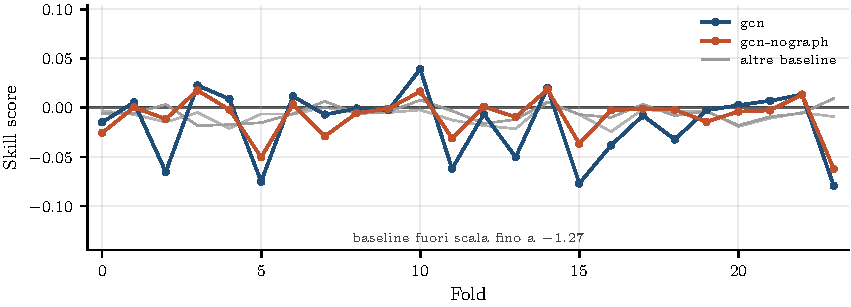
\includegraphics[width=\textwidth]{figures/fig_results_by_fold.pdf}
\caption[Skill score per fold]{Skill score contro la previsione nulla, fold per fold, per i due bracci della GCN e le baseline. La scala verticale è calibrata sui due bracci evidenziati. Le baseline che escono dall'intervallo sono annotate con il loro valore peggiore.}
\label{fig:tc-results-by-fold}
\end{figure}

\subsection{Densità del grafo e skill score}

La \Cref{sec:known-limitations-gnn} ha osservato che su un grafo denso l'over-smoothing si manifesta a profondità minore. Il \Cref{ch:topological-evolution} ha mostrato che il grafo dello studio è quasi completo e che si compatta attorno alle crisi. Si verifica quindi un'ipotesi che incrocia le due questioni di ricerca, ovvero se nei fold in cui il grafo è più denso la GCN preveda peggio.

Questa associazione è misurata dalla correlazione di rango di Spearman. La scelta del coefficiente è motivata da due ragioni fondamentali: l'ipotesi afferma una monotonicità e non una forma funzionale, che è esattamente ciò che una correlazione di rango quantifica; e alla soglia calibrata $8$ fold su $24$ hanno densità media esattamente pari a $1$, un blocco di pari merito a cui i ranghi assegnano il rango medio, con una spaziatura unitaria che limita l'influenza dei fold più distanti.

La retta mostrata nella \cref{fig:tc-density-vs-error} è la stima di Theil-Sen, cioè la mediana delle pendenze tra coppie di punti. Il risultato è $\rho=-0{,}100$ ($p=0{,}643$) alla soglia calibrata e $\rho=0{,}005$ ($p=0{,}981$) alla soglia $\tau_{\mathrm{FWER}}$, dove nessun fold satura. Nessuna delle due associazioni è distinguibile da zero, esito interpretabile come un test a bassa potenza e non come una confutazione. Alla soglia calibrata, inoltre, la densità media per fold varia solo tra $0{,}887$ e $1{,}000$, comprimendo proprio la variazione di cui il test avrebbe bisogno.

\begin{figure}[H]
\centering
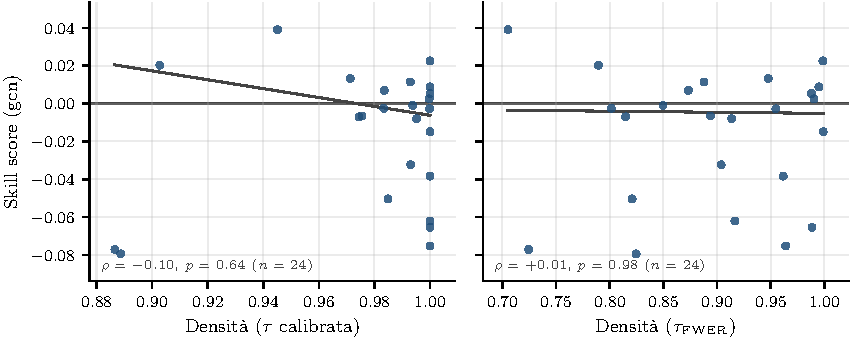
\includegraphics[width=\textwidth]{figures/fig_density_vs_error.pdf}
\caption[Densità del grafo e skill score della GCN]{Skill score della GCN contro la densità media del grafo nel blocco di test, per fold, alle soglie $\tau$ e $\tau_{\mathrm{FWER}}$. La retta è la stima di Theil-Sen.}
\label{fig:tc-density-vs-error}
\end{figure}

Il protocollo walk-forward, la griglia fissata a priori e la correzione per confronti multipli lasciano poco margine per orientare il confronto verso un esito favorevole. L'esito è negativo: nessuno dei sei modelli batte la baseline \texttt{ZeroForecaster} sui rendimenti giornalieri, e la GCN non si distingue in modo statisticamente significativo né da essa né dalla propria ablation senza grafo.

% ============================================================
% CAPITOLO 6 — Il backtest
% Scritto il 2026-09-13 seguendo il programma in frontmatter/abstract.tex.
% Copre scripts/06_run_backtest.py e src/cryptognn/evaluation/backtest.py.
% Assorbe YYY_literature-review.tex (sec:evaluation-metrics-methodological-
% pitfalls, "Scelta della metrica di valutazione") e ZZZ_old-case-study.tex
% ("Il costo economico"). Decisioni di sessione:
%   - Label con prefisso bt- e tabella ricopiata inline (non
%     \begin{table}[H]
\centering
\caption[Metriche economiche della strategia sul segno]{Strategia sul segno della previsione, equipesata sui 15 asset e ribilanciata ogni giorno, sui $1\,512$ giorni del periodo di test. Ogni misura è riportata a 0 e a 10 punti base di costo, applicati a ogni cambio di posizione; lo Sharpe è annualizzato su 365 giorni e non sottrae un tasso privo di rischio. Il buy-and-hold è il paniere equipesato acquistato il primo giorno e mantenuto, e non usa alcuna previsione: serve da termine di paragone. La previsione nulla non prende posizione, quindi il suo Sharpe non è definito.}
\label{tab:backtest}
\small
\begin{tabular}{@{}lrrrrrr@{}}
\toprule
 & \multicolumn{2}{c}{\textbf{Sharpe}} & \multicolumn{2}{c}{\textbf{Max drawdown}} & \multicolumn{2}{c}{\textbf{Rend. cumulato}} \\
\cmidrule(lr){2-3}\cmidrule(lr){4-5}\cmidrule(lr){6-7}
\textbf{Modello} & \textbf{0 bps} & \textbf{10 bps} & \textbf{0 bps} & \textbf{10 bps} & \textbf{0 bps} & \textbf{10 bps} \\
\midrule
Zero & -- & -- & $0{,}0\%$ & $0{,}0\%$ & $0{,}0\%$ & $0{,}0\%$ \\
Media storica & $-0{,}665$ & $-0{,}671$ & $-84{,}4\%$ & $-84{,}5\%$ & $-80{,}5\%$ & $-80{,}7\%$ \\
AR & $-0{,}596$ & $-0{,}718$ & $-79{,}1\%$ & $-82{,}9\%$ & $-75{,}6\%$ & $-80{,}3\%$ \\
VAR (BIC) & $-0{,}665$ & $-0{,}671$ & $-84{,}4\%$ & $-84{,}5\%$ & $-80{,}5\%$ & $-80{,}7\%$ \\
VAR ($p=5$) & $0{,}147$ & $-0{,}612$ & $-60{,}6\%$ & $-87{,}0\%$ & $-16{,}2\%$ & $-81{,}2\%$ \\
GCN & $0{,}453$ & $0{,}014$ & $-66{,}0\%$ & $-83{,}8\%$ & $43{,}1\%$ & $-55{,}1\%$ \\
GCN senza grafo & $0{,}610$ & $0{,}051$ & $-44{,}2\%$ & $-59{,}3\%$ & $108{,}2\%$ & $-31{,}5\%$ \\
Buy-and-hold & $0{,}262$ & $0{,}261$ & $-66{,}9\%$ & $-66{,}9\%$ & $-14{,}7\%$ & $-14{,}8\%$ \\
\bottomrule
\end{tabular}
\end{table}
) perché ZZZ, ancora \input, definisce già
%     tab:backtest e fig:equity-curves.
%   - Alla tabella generata è aggiunta la colonna del turnover medio, presa
%     da project-thesis/results/summary.md: la lettura dei risultati si regge
%     su quella colonna.
%   - report() di 06_run_backtest.py è descritto in prosa, senza snippet.
%   - Nei blocchi minted le omissioni rispetto al sorgente sono segnate da
%     "# ..."; per il resto il codice è verbatim.
% ============================================================
\chapter{Il backtest}
\label{ch:backtest}

Il \Cref{ch:training-and-comparison} si è chiuso con un esito negativo: nessuno dei sei modelli batte la baseline \texttt{ZeroForecaster} in errore quadratico, e la GCN non si distingue dalla propria ablation. Questo verdetto riguarda però l'accuratezza, e non consente di trarre conclusioni sul valore delle previsioni per chi le usa. I due risultati non devono necessariamente coincidere: l'errore quadratico è dominato dalle giornate in cui una previsione sbaglia maggiormente, mentre una strategia che opera sul suo segno tiene conto solamente della direzione. Un modello può quindi avere l'RMSE peggiore, ma la strategia migliore. Questo capitolo misura il valore economico delle previsioni seguendo lo script \path{06_run_backtest.py}.

\section{Oltre l'errore di previsione}
\label{sec:bt-beyond-accuracy}

L'RMSE e il MAE sono metriche standard per la regressione, poco informative però sui rendimenti finanziari. Il motivo discende direttamente dagli \emph{stylized facts} della \cref{sec:stylized-facts}: i rendimenti hanno media prossima a zero e un'autocorrelazione lineare di intensità contenuta, quindi il predittore costante $\hat r=0$ ottiene già un RMSE vicino a quello ottimo. Sul periodo di test dello studio vale $0{,}04145$ (\cref{tab:tc-results-main}). Un modello può ridurre questo valore di una frazione di punto percentuale senza che il miglioramento si distingua dal rumore. Un RMSE eccellente, inoltre, è compatibile con un modello che sbaglia sistematicamente il segno.

L'accuratezza direzionale misura ciò che serve per applicare il modello ai casi reali, ma tratta allo stesso modo un movimento dello $0{,}1\%$ e uno del $20\%$. Un modello può quindi predire correttamente il segno nel $60\%$ dei casi e perdere comunque denaro se sbaglia proprio nelle giornate che contano.

Le metriche economiche rispondono direttamente alla domanda rilevante per un investitore, ovvero se le previsioni producano un profitto al netto dei costi. Si costruisce una strategia che opera sulle previsioni e se ne misurano il rendimento cumulato, il rendimento in rapporto alla volatilità e la perdita peggiore subita. Queste metriche dipendono però da ipotesi come quella sui costi di transazione, dichiarata esplicitamente dalla pipeline.

\section{Le misure di performance}
\label{sec:bt-metrics}

\subsection{Sharpe ratio}
\label{sec:bt-sharpe}

Sia $x_1,\dots,x_n$ la serie dei rendimenti giornalieri di una strategia. Lo Sharpe ratio~\cite{sharpe1966mutual,sharpe1994sharpe} adottato dallo studio rapporta il rendimento medio alla sua variabilità,
\begin{equation}
\label{eq:bt-sharpe}
\mathrm{SR}=\sqrt{P}\,\frac{\bar x}{s},\qquad \bar x=\frac1n\sum_{t=1}^n x_t,\qquad s^2=\frac{1}{n-1}\sum_{t=1}^n(x_t-\bar x)^2,
\end{equation}
dove $P$ è il numero di periodi in un anno. Il fattore $\sqrt{P}$ annualizza il rapporto. La media cresce infatti linearmente con l'orizzonte e la deviazione standard con la sua radice, se i rendimenti sono indipendenti. Lo Sharpe ratio quantifica il rendimento medio per unità di rischio, dove il rischio è identificato con la deviazione standard dei rendimenti. Non misura quindi la redditività assoluta della strategia, ma la sua efficienza nell'impiego della volatilità sostenuta. A parità di $\bar x$, un incremento della dispersione $s$ riduce proporzionalmente l'indicatore, penalizzando le strategie il cui rendimento deriva da oscillazioni di ampiezza elevata.

\begin{listing}[H]
\begin{minted}{python}
def sharpe(returns: np.ndarray, periods: int = PERIODS_PER_YEAR) -> float:
    returns = np.asarray(returns, dtype=float)
    # Check the series is one-dimensional and the periods per year are positive.
    ...
    if returns.size < 2:
        return float("nan")

    deviation = float(returns.std(ddof=1))
    if deviation == 0.0:
        return float("nan")
    return float(returns.mean() / deviation * np.sqrt(periods))
\end{minted}
\caption{\texttt{sharpe}}
\label{lst:sharpe}
\end{listing}

Nella definizione originale~\cite{sharpe1966mutual}, il numeratore corrisponde al rendimento in eccesso della strategia rispetto ad un'attività priva di rischio: detto $r_{f,t}$ il rendimento di quest'ultima nel periodo $t$ e posto $x_{e,t}=x_t-r_{f,t}$, lo Sharpe ratio è
\[
\mathrm{SR}_e=\sqrt{P}\,\frac{\bar x_e}{s_e},\qquad
\bar x_e=\frac1n\sum_{t=1}^n x_{e,t},\qquad
s_e^2=\frac{1}{n-1}\sum_{t=1}^n(x_{e,t}-\bar x_e)^2.
\]
L'equazione~\eqref{eq:bt-sharpe}, che la funzione implementa, ne è il caso particolare $r_{f,t}=0$ per ogni $t$. La pipeline adotta tale variante perché, tra il 2022 e il 2026, il tasso a breve è passato da valori prossimi a zero a circa il $5\%$; pertanto un valore unico sarebbe sbagliato per gran parte del campione.

La costante \texttt{PERIODS\_PER\_YEAR} vale $365$ e non $252$. Come accennato nella \cref{sec:stylized-facts}, il mercato delle criptovalute non è soggetto ad interruzioni o pause e non ci sono giornate da escludere. Usare $252$ ridurrebbe tutti gli Sharpe ratio di un fattore $\sqrt{252/365}\approx0{,}83$.

Una serie costante, inoltre, ha deviazione standard nulla e l'equazione~\eqref{eq:bt-sharpe} non è definita. La funzione restituisce allora \texttt{NaN}, allineandosi al caso della previsione nulla che non prende mai posizione e ha tutti i rendimenti giornalieri nulli. Uno Sharpe pari a $0$ si leggerebbe come una strategia dal rendimento piatto, quando invece la strategia non esiste. La convenzione è la stessa già adottata dall'accuratezza direzionale nella \cref{sec:tc-skill-score}.

\subsection{Massimo drawdown}
\label{sec:bt-drawdown}

Sia $E_0,\dots,E_n$ la curva del capitale, ottenuta reinvestendo integralmente il risultato di ogni periodo: posto $E_0=1$, il capitale evolve secondo la ricorsione $E_t=E_{t-1}(1+x_t)$, cosicché $E_t$ è il valore di un investimento unitario iniziale dopo $t$ periodi. Esplicitando la ricorsione si ottiene la forma moltiplicativa
\[
E_t=\prod_{i=1}^{t}(1+x_i),\qquad t=0,\dots,n,
\]
con la convenzione che il prodotto vuoto valga $1$. La composizione è moltiplicativa, motivo per cui una perdita e un guadagno di pari entità percentuale non si compensano.

Si definisce drawdown all'istante $t$ lo scostamento relativo del capitale dal massimo raggiunto fino a quell'istante, $D_t=\dfrac{E_t}{\max_{0\leq s\leq t}E_s}-1$. Il massimo drawdown è il minimo corrente di tale successione,
\begin{equation}
\label{eq:bt-max-drawdown}
\mathrm{MDD}=\min_{0\leq t\leq n}D_t=\min_{0\leq t\leq n}\left(\frac{\max(E_t,0)}{\max_{0\leq s\leq t}E_s}-1\right).
\end{equation}
È un numero compreso tra $-1$ e $0$: vale $0$ per una curva che non scende mai sotto il proprio massimo precedente e tende a $-1$ quando il capitale viene eroso quasi per intero. Misura la peggiore perdita che un investitore avrebbe sperimentato entrando nel momento meno favorevole, ovvero l'ampiezza massima della fase di ritracciamento subita dalla strategia sull'intero periodo.

\begin{listing}[H]
\begin{minted}{python}
def max_drawdown(equity: np.ndarray) -> float:
    equity = np.asarray(equity, dtype=float)
    # Check the curve is one-dimensional and return NaN if it is empty.
    ...
    peak = np.maximum.accumulate(equity)
    if peak[0] <= 0:
        raise ValueError(f"Equity curve starts at {equity[0]}: a drawdown needs positive capital to fall from")
    return float(np.min(np.maximum(equity, 0.0) / peak - 1.0))
\end{minted}
\caption{\texttt{max\_drawdown}}
\label{lst:max-drawdown}
\end{listing}

Il massimo cumulato \texttt{np.maximum.accumulate} calcola il picco $\max_{s\leq t}E_s$ per ogni $t$ in un solo passaggio. Il picco parte dal primo elemento della serie ricevuta: se la curva cominciasse da $E_1$ anziché da $E_0$, il picco iniziale coinciderebbe con $E_1$ e la caduta da $E_0$ a $E_1$ non verrebbe mai contata. Per questo, la funzione che riassume una strategia antepone il capitale iniziale $E_0=1$, con \texttt{np.concatenate(([1.0], equity))}. Il termine \texttt{np.maximum(equity, 0.0)} realizza il pavimento a $-1$ dell'equazione~\eqref{eq:bt-max-drawdown}. Una strategia che vende allo scoperto può in linea di principio perdere più del proprio capitale. Oltre la perdita totale non resta però nulla da perdere e un drawdown di $-1{,}4$ non avrebbe significato.

\section{La strategia sul segno}
\label{sec:bt-strategy}

Per trasformare le previsioni in rendimenti è necessaria una strategia. Sia $\hat r_{t,i}$ la previsione del log-rendimento dell'asset $i$ realizzato nel giorno $t$. Quella adottata dal progetto assume ogni giorno su ciascuno degli $N=15$ asset una posizione lunga (\emph{long}) se la previsione è positiva e corta (\emph{short}) se è negativa, con peso
\begin{equation}
\label{eq:bt-weights}
w_{t,i}=\frac{\operatorname{sign}(\hat r_{t,i})}{N}.
\end{equation}
Il portafoglio è equipesato e ribilanciato ogni giorno. Non interviene alcuna ottimizzazione: non si dimensionano le posizioni in base alla fiducia nella previsione, non si controlla la volatilità e non si scelgono gli asset su cui operare.

Il denominatore è $N$ fisso e non il numero di posizioni diverse da zero. L'esposizione lorda $\sum_i|w_{t,i}|$ resta in questo modo al più $1$ e le curve dei diversi modelli sono confrontabili. Normalizzare per il numero di posizioni attive aumenterebbe la leva di un modello proprio nei giorni in cui è indeciso.

Le posizioni sono applicate ai rendimenti semplici, non ai log-rendimenti. La \cref{sec:returns-stationarity} ha mostrato che le due grandezze coincidono solo per variazioni piccole. Una posizione corta non guadagna $-r_{t,i}$ ma $-R_{t,i}=-(e^{r_{t,i}}-1)$. Sulla giornata da $-30\%$ del \cref{ch:dynamic-correlation-graph}, con $r=-0{,}357$, una posizione corta guadagna il $30\%$ e non il $35{,}7\%$. Il rendimento lordo della strategia è quindi
\begin{equation}
\label{eq:bt-gross-return}
x_t^{\mathrm{lordo}}=\sum_{i=1}^N w_{t,i}\,R_{t,i},\qquad R_{t,i}=e^{r_{t,i}}-1.
\end{equation}

L'equazione~\eqref{eq:bt-weights} è implementata da \texttt{sign\_strategy} (\cref{lst:sign-strategy}), che riceve la tabella delle previsioni prodotta da \texttt{run\_walkforward} (\cref{sec:tc-walkforward}), con una riga per data, asset e modello.

\begin{listing}[H]
\begin{minted}{python}
def sign_strategy(predictions: pd.DataFrame, cost_bps: float) -> pd.DataFrame:
    forecast = _panel(predictions, "y_pred")
    realized = np.expm1(_panel(predictions, "y_true"))
    return _curve(np.sign(forecast) / forecast.shape[1], realized, cost_bps)
\end{minted}
\caption{\texttt{sign\_strategy}}
\label{lst:sign-strategy}
\end{listing}

La funzione ausiliaria \texttt{\_panel} converte il DataFrame \texttt{predictions} in una matrice di $\mathbb{R}^{n\times N}$, con una riga per data e una colonna per asset, e solleva un errore se manca anche solo una cella. Un valore mancante produrrebbe un rendimento \texttt{NaN} che, propagato nel prodotto cumulato, svuoterebbe l'intera curva da quel giorno in poi. I rendimenti semplici sono ottenuti con \texttt{np.expm1}, che calcola $e^r-1$ senza perdita di precisione per $r$ piccolo. Il costo non è direttamente utilizzato da \texttt{sign\_strategy}, che si occupa di inoltrarlo alla funzione \texttt{\_curve} (\cref{lst:curve}), la quale lo addebita secondo la \cref{sec:bt-cost}.

Il rendimento realizzato, inoltre, non è passato come argomento separato. La tabella contiene già \texttt{y\_true} e \texttt{y\_pred} sulla stessa riga e una seconda fonte potrebbe introdurre un disallineamento, errore che non produrrebbe un'eccezione ma renderebbe la curva plausibile e sbagliata.

\section{Il riferimento buy-and-hold}
\label{sec:bt-benchmark}

Le misure di una singola strategia non sono interpretabili in assoluto, ma solo rispetto al mercato sugli stessi giorni. Serve quindi un termine di paragone che non usi alcuna previsione, costruito da \texttt{buy\_and\_hold} (\cref{lst:buy-and-hold}).

\begin{listing}[H]
\begin{minted}{python}
def buy_and_hold(predictions: pd.DataFrame, cost_bps: float) -> pd.DataFrame:
    realized = np.expm1(_panel(predictions.drop_duplicates(["date", "asset"]), "y_true"))
    positions = pd.DataFrame(1.0 / realized.shape[1], index=realized.index, columns=realized.columns)
    return _curve(positions, realized, cost_bps)
\end{minted}
\caption{\texttt{buy\_and\_hold}}
\label{lst:buy-and-hold}
\end{listing}

Il buy-and-hold assume una posizione lunga di peso $1/N$ su ogni asset per l'intero periodo. È l'unica strategia della tabella che non usa alcuna previsione. Poiché i pesi non cambiano mai, il suo turnover è $1$ il primo giorno e $0$ in tutti gli altri.

\section{Costi e curva del capitale}
\label{sec:bt-costs-and-curve}

\subsection{Il costo di transazione}
\label{sec:bt-cost}

Ogni cambio di posizione ha un costo, dovuto alle commissioni applicate dall'exchange, al differenziale tra denaro e lettera (\emph{bid-ask spread}) e allo scostamento tra il prezzo atteso e quello di effettiva esecuzione (\emph{slippage}). Il turnover del giorno $t$ misura quanto il portafoglio è cambiato rispetto al giorno precedente,
\begin{equation}
\label{eq:bt-turnover}
u_t=\sum_{i=1}^N\left|w_{t,i}-w_{t-1,i}\right|,\qquad w_{0,i}=0.
\end{equation}
Il portafoglio parte vuoto, quindi il primo giorno paga l'ingresso come qualunque altro cambio di posizione. Il costo è proporzionale al turnover secondo un'aliquota $c$ espressa in \emph{basis point}, ovvero in centesimi di punto percentuale. È l'unità in cui le borse pubblicano le proprie commissioni. Il rendimento netto e il capitale sono
\begin{equation}
\label{eq:bt-net-return}
x_t=x_t^{\mathrm{lordo}}-c\cdot10^{-4}\,u_t,\qquad E_t=\prod_{s=1}^t(1+x_s).
\end{equation}
Un modello che inverte il segno di tutte le previsioni da un giorno all'altro ha $u_t=2$ e paga $2c$ basis point. Un modello che non cambia mai posizione paga solo l'ingresso. Il turnover è calcolato sui pesi e non tiene conto della deriva delle posizioni dovuta ai rendimenti del giorno. Il ribilanciamento verso pesi uguali non viene quindi addebitato, una semplificazione che vale allo stesso modo per tutte le strategie.

\subsection{Dalle posizioni al capitale}
\label{sec:bt-curve}

La strategia sul segno e il buy-and-hold passano dalla stessa funzione \texttt{\_curve}, che implementa le equazioni~\eqref{eq:bt-gross-return}, \eqref{eq:bt-turnover} e~\eqref{eq:bt-net-return}.

\begin{listing}[H]
\begin{minted}{python}
def _curve(positions: pd.DataFrame, simple_returns: pd.DataFrame, cost_bps: float) -> pd.DataFrame:
    if cost_bps < 0:
        raise ValueError(f"Transaction cost must be non-negative, got {cost_bps} bps")

    gross = (positions * simple_returns).sum(axis=1)
    turnover = (positions - positions.shift(1).fillna(0.0)).abs().sum(axis=1)
    cost = turnover * cost_bps * BASIS_POINT
    net = gross - cost

    return pd.DataFrame(
        {
            "date": positions.index,
            "gross_return": gross.to_numpy(),
            "turnover": turnover.to_numpy(),
            "cost": cost.to_numpy(),
            "net_return": net.to_numpy(),
            "equity": (1.0 + net).cumprod().to_numpy(),
        }
    )
\end{minted}
\caption{\texttt{\_curve}}
\label{lst:curve}
\end{listing}

Il prodotto \texttt{positions * simple\_returns} è elemento per elemento e la somma per riga restituisce $x_t^{\mathrm{lordo}}$. L'istruzione \texttt{positions.shift(1).fillna(0.0)} costruisce $w_{t-1,i}$, con il valore nullo del primo giorno, che corrisponde a $w_{0,i}=0$. La costante \texttt{BASIS\_POINT} vale $10^{-4}$ ed è utilizzata per convertire \texttt{cost\_bps} da basis point a frazione del capitale. Il capitale è il prodotto cumulato di $1+x_t$. La posizione non viene chiusa l'ultimo giorno, perché liquidare alla fine del campione non è una decisione della strategia. Condividere \texttt{\_curve} tra le due strategie garantisce che la contabilità dei costi sia identica per il modello misurato e per il suo termine di paragone.

\section{Risultati}
\label{sec:bt-results}

La \Cref{tab:bt-backtest} riporta le misure delle otto strategie valutate — i sette modelli del \cref{ch:training-and-comparison}, ciascuno attraverso la strategia sul segno, e il buy-and-hold — sui $1512$ giorni del periodo di test, dal 05/05/2022 al 24/06/2026, ai due livelli di costo. Le previsioni non sono ricalcolate in questa fase, ma sono quelle fissate dagli addestramenti del \cref{ch:training-and-comparison} e rilette dal disco.

Il livello di costo positivo, che vale $10$ basis point nella pipeline di progetto, e quello nullo sono valutati nella stessa esecuzione. La distanza tra gli Sharpe a costi diversi, che corrisponde all'informazione da ricavare, è più affidabile se le sue parti provengono dallo stesso codice applicato agli stessi giorni.

\begin{table}[H]
\centering
\caption[Metriche economiche della strategia sul segno]{Strategia sul segno della previsione, equipesata sui $15$ asset e ribilanciata ogni giorno, sui $1\,512$ giorni del periodo di test, a $0$ e a $10$ basis point di costo. Lo Sharpe è annualizzato su $365$ giorni e non sottrae un tasso privo di rischio. Il turnover è la media giornaliera e non dipende dal costo. Il buy-and-hold non usa alcuna previsione e serve da termine di paragone. La previsione nulla non prende posizione, quindi il suo Sharpe non è definito.}
\label{tab:bt-backtest}
\small
\setlength{\tabcolsep}{4pt}
\begin{tabular}{@{}lrrrrrrr@{}}
\toprule
 & \multicolumn{2}{c}{\textbf{Sharpe}} & \multicolumn{2}{c}{\textbf{Max drawdown}} & \multicolumn{2}{c}{\textbf{Rend. cumulato}} & \\
\cmidrule(lr){2-3}\cmidrule(lr){4-5}\cmidrule(lr){6-7}
\textbf{Modello} & \textbf{0 bps} & \textbf{10 bps} & \textbf{0 bps} & \textbf{10 bps} & \textbf{0 bps} & \textbf{10 bps} & \textbf{Turnover} \\
\midrule
Zero & -- & -- & $0{,}0\%$ & $0{,}0\%$ & $0{,}0\%$ & $0{,}0\%$ & $0{,}000$ \\
Media storica & $-0{,}665$ & $-0{,}671$ & $-84{,}4\%$ & $-84{,}5\%$ & $-80{,}5\%$ & $-80{,}7\%$ & $0{,}007$ \\
AR & $-0{,}596$ & $-0{,}718$ & $-79{,}1\%$ & $-82{,}9\%$ & $-75{,}6\%$ & $-80{,}3\%$ & $0{,}141$ \\
VAR (BIC) & $-0{,}665$ & $-0{,}671$ & $-84{,}4\%$ & $-84{,}5\%$ & $-80{,}5\%$ & $-80{,}7\%$ & $0{,}007$ \\
VAR ($p=5$) & $0{,}147$ & $-0{,}612$ & $-60{,}6\%$ & $-87{,}0\%$ & $-16{,}2\%$ & $-81{,}2\%$ & $0{,}987$ \\
GCN & $0{,}453$ & $0{,}014$ & $-66{,}0\%$ & $-83{,}8\%$ & $43{,}1\%$ & $-55{,}1\%$ & $0{,}766$ \\
GCN senza grafo & $0{,}610$ & $0{,}051$ & $-44{,}2\%$ & $-59{,}3\%$ & $108{,}2\%$ & $-31{,}5\%$ & $0{,}735$ \\
Buy-and-hold & $0{,}262$ & $0{,}261$ & $-66{,}9\%$ & $-66{,}9\%$ & $-14{,}7\%$ & $-14{,}8\%$ & $0{,}001$ \\
\bottomrule
\end{tabular}
\end{table}

\subsection{Senza costi di transazione}

Senza costi di transazione, la GCN e la sua ablation ottengono gli Sharpe ratio più alti della tabella, rispettivamente $0{,}453$ e $0{,}610$, superando il buy-and-hold ($0{,}262$). Il rendimento è del $43{,}1\%$ per la GCN e del $108{,}2\%$ per la variante senza grafo, a fronte del $-14{,}7\%$ del portafoglio di riferimento. La variante senza grafo ha anche il drawdown meno profondo, $-44{,}2\%$ contro il $-66{,}0\%$ della GCN. Il VAR con ordine fissato ha uno Sharpe appena positivo ($0{,}147$). Le altre baseline perdono in modo consistente.

Il risultato non contraddice il \cref{ch:training-and-comparison}. La GCN ha lo skill score peggiore tra i due bracci e un'accuratezza direzionale del $50{,}9\%$, ma la strategia sul segno è insensibile all'ampiezza degli errori: conta solo che le giornate in cui il segno è corretto coincidano con movimenti ampi.

La media storica e il VAR selezionato per BIC producono righe identiche, perché coincidono numericamente (\cref{sec:var-baseline}). La loro previsione è costante all'interno di ciascun fold, quindi le posizioni cambiano solo al passaggio da un fold al successivo e il turnover medio è di appena $0{,}007$. La previsione nulla non prende mai posizione: il suo capitale resta pari a $1$ e lo Sharpe non è definito.

Il buy-and-hold mostra che le misure della tabella non vanno lette isolatamente: il suo Sharpe è positivo mentre il rendimento cumulato è negativo. Lo Sharpe usa la media aritmetica dei rendimenti giornalieri, mentre il capitale li compone in modo geometrico. Con una volatilità elevata come quella delle criptovalute la differenza tra le due medie è ampia. Una sequenza di $+50\%$ e $-50\%$ ha media aritmetica nulla ma riduce il capitale a $0{,}75$.

\subsection{Con i costi di transazione}

\begin{figure}[H]
\centering
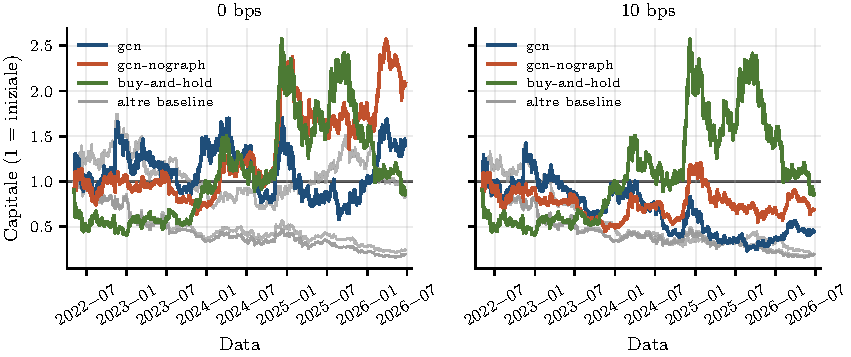
\includegraphics[width=\textwidth]{figures/fig_equity_curves.pdf}
\caption[Curve del capitale della strategia sul segno]{Capitale della strategia sul segno nel periodo di test, a $0$ e a $10$ basis point di costo, sullo stesso asse verticale. Sono evidenziati i due bracci della GCN e il buy-and-hold. Le altre baseline sono in grigio.}
\label{fig:bt-equity-curves}
\end{figure}

A $10$ basis point la classifica si inverte. Lo Sharpe della GCN scende da $0{,}453$ a $0{,}014$ e quello della variante senza grafo da $0{,}610$ a $0{,}051$. Il buy-and-hold resta pressoché invariato a $0{,}261$. Il rendimento cumulato dei due bracci diventa negativo, $-55{,}1\%$ e $-31{,}5\%$. La \Cref{fig:bt-equity-curves} mostra la stessa erosione nel tempo: a costo zero le curve dei due bracci terminano sopra il capitale iniziale; con i costi scivolano entrambe sotto di esso, mentre la curva del portafoglio di riferimento è la stessa nei due pannelli.

La colonna del turnover spiega il ribaltamento. Le reti cambiano posizione quasi ogni giorno, con un turnover medio di $0{,}766$ per la GCN e $0{,}735$ per la variante senza grafo. Per l'equazione~\eqref{eq:bt-net-return} questo costa in media circa $7{,}5$ basis point al giorno, cioè oltre il $27\%$ del capitale all'anno prima di ogni composizione. Il VAR con ordine fissato ha il turnover più alto, $0{,}987$. Il suo Sharpe passa da $0{,}147$ a $-0{,}612$. All'estremo opposto il buy-and-hold paga solo l'ingresso ($0{,}001$) e la media storica solo i cambi di fold ($0{,}007$). L'AR, con un turnover intermedio di $0{,}141$, perde $0{,}12$ di Sharpe.

Il confronto tra i due Sharpe classifica ciascun modello. La GCN e la sua ablation sopravvivono al costo, restando positive anche al netto, ma con $0{,}014$ e $0{,}051$ che non si distinguono da zero in alcun senso pratico. Per il VAR con ordine fissato il costo consuma l'intero vantaggio, perché il suo Sharpe è positivo solo a costo nullo. Media storica, AR e VAR selezionato per BIC sono in perdita a entrambi i livelli. Il confronto decisivo resta però quello con il buy-and-hold: il modello migliore, al netto dei costi, è la GCN senza grafo, con uno Sharpe di $0{,}051$ che rimane sotto lo $0{,}261$ del riferimento.

\subsection{Il verdetto economico}

Il backtest conferma sul piano economico l'esito del \cref{ch:training-and-comparison}. A costo zero, la strategia sulle previsioni delle reti appare migliore del mercato; è però sufficiente un costo modesto di $10$ basis point per cambio di posizione a eliminare il vantaggio, perché il segnale è più piccolo del costo necessario a sfruttarlo. Al netto dei costi, nessun modello è preferibile al semplice acquisto dei quindici asset, rischio segnalato nella \cref{sec:bt-beyond-accuracy}.

Il risultato ha però limiti precisi. Il costo modellato è una commissione proporzionale, senza slippage né limiti di capienza del mercato, quindi le frizioni reali sarebbero più alte. Gli Sharpe ratio sono inoltre stimati su un unico periodo e la strategia è deliberatamente semplice. Una strategia che filtra le previsioni più deboli ridurrebbe il turnover, ma introdurrebbe proprio i gradi di libertà che lo studio ha scelto di non avere.

% ============================================================
% CAPITOLO 7 — Conclusioni e sviluppi futuri
% Riscritto il 2026-09-17 sui risultati dei Cap. 4, 5 e 6.
% Sostituisce la versione pre-ristrutturazione. Decisioni di sessione:
%   - La prima questione non è più "cosa dice la letteratura" ma l'esito
%     empirico dei Cap. 5/6: ogni riferimento alla rassegna è rimosso.
%   - La derivazione della GCN è riassunta come nel Cap. 2 attuale
%     (località, pesi condivisi, equivarianza, self-loop, normalizzazione,
%     renormalization trick): niente Chebyshev né base di autovettori U.
%   - Prosa quantitativa: le cifre decisive sono in linea, senza
%     introdurre tabelle o figure nuove in questo capitolo.
%   - Subsection numerate (erano \subsection*), per coerenza coi Cap. 4-7.
% ============================================================
\chapter{Conclusioni e sviluppi futuri}
\label{ch:conclusions}

\section{Sintesi rispetto alle questioni di ricerca}
\label{sec:summary-research-questions}

La \Cref{sec:objectives-research-questions} dell'Introduzione ha formulato due questioni: quale vantaggio predittivo offra la struttura relazionale tra criptovalute rispetto ad un approccio che le tratti come asset indipendenti e come quella struttura si trasformi nel passaggio da un mercato stabile ad uno di crisi. I capitoli precedenti hanno costruito gli strumenti per affrontarle e ne hanno misurato le risposte; questa sezione ne offre una sintesi unitaria.

\subsection{Il vantaggio della struttura}

Il \Cref{ch:forecasting-models} ha derivato la GCN dalle sole proprietà di località, condivisione dei pesi ed equivarianza per permutazione, come modo per recuperare l'informazione che un approccio univariato scarta per costruzione. I parametri $W^{(l)}$ agiscono sullo spazio delle feature e non sui nodi (\cref{sec:gcn-kipf-welling}), il che consente di applicare lo stesso layer ad un grafo che si ricostruisce ad ogni finestra (\cref{sec:dynamic-graphs-temporal-question}).

Sui dati, però, quell'informazione non si traduce in previsione. Nel \Cref{ch:training-and-comparison} nessuno dei sei modelli batte la previsione nulla, e la GCN non se ne distingue nemmeno dopo la correzione di Holm ($p_{\mathrm{Holm}}=0{,}683$); il confronto con la propria ablation senza grafo, forma più diretta della questione, restituisce $\mathrm{DM}=1{,}338$ con $p=0{,}181$, e il segno indica nel braccio dotato di grafo il meno accurato dei due. Le scomposizioni per asset e per fold confermano il quadro e l'accuratezza direzionale non supera mai il $51{,}2\%$.

L'esito non dipende dalla sola rete. Il BIC riduce quasi sempre AR e VAR al caso degenere di ordine nullo (\cref{sec:var-baseline}) e la griglia della GCN restituisce celle indistinguibili tra loro (\cref{tab:tc-gcn-grid}).

Il \Cref{ch:backtest} raggiunge lo stesso punto per via economica. A costo nullo la strategia sul segno delle previsioni supera il buy-and-hold, con Sharpe $0{,}453$ per la GCN e $0{,}610$ per la sua ablation contro $0{,}262$; bastano $10$ basis point per cambio di posizione a ridurli a $0{,}014$ e $0{,}051$, mentre il riferimento resta a $0{,}261$. Con un turnover prossimo a $0{,}75$ il segnale costa più di quanto renda.

Il protocollo, dal walk-forward alla griglia fissata in anticipo fino alla correzione per confronti multipli, non lasciava margine per orientare il confronto verso un esito favorevole: è questo a rendere informativo il risultato negativo. Alla frequenza giornaliera e ad un passo, su quindici criptovalute, la struttura relazionale non offre un vantaggio predittivo misurabile.

\subsection{L'evoluzione della struttura}

Il \Cref{ch:graph-laplacian-theory} ha legato ogni autovalore all'irregolarità del proprio autovettore (\cref{sec:spectral-analysis}), dando un significato preciso alla connettività algebrica $\lambda_2$: cresce quando il grafo diventa difficile da separare in gruppi distinti, cioè quando il mercato smette di articolarsi e si muove in blocco. È una misura del compattamento che non richiede una soglia e che dipende da come i pesi sono distribuiti sulla struttura, non dal loro solo livello medio.

Il \Cref{ch:topological-evolution} l'ha applicata, con altre cinque metriche, alle $1947$ finestre del periodo, trovando un mercato compatto in permanenza: la correlazione media vale $0{,}675$ sull'intero campione, la quota del modo di mercato $0{,}711$, e un solo autovalore eccede il bordo di Marchenko--Pastur in $1939$ finestre su $1947$. Oltre il modo comune a tutti gli asset, la matrice di correlazione empirica non contiene struttura che il rumore di stima non basti a spiegare.

Attorno alla stretta cinese del maggio 2021 ogni metrica si muove nella direzione attesa e quasi ognuna raggiunge un estremo della propria distribuzione storica, con la correlazione media che raddoppia tra la finestra interamente precedente e quella interamente successiva. Terra/Luna e FTX spostano le stesse quantità di pochi punti percentuali, perché a sessanta giorni dai due eventi la correlazione media valeva già $0{,}799$ e $0{,}753$ e il grafo filtrato alla soglia calibrata era completo ad ogni offset letto. Nel 2022 il mercato si trovava già nello stato verso cui una crisi lo spingerebbe, e una metrica vicina al proprio estremo ha poco margine per muoversi. Il compattamento in crisi è confermato, ma come fenomeno di livello prima che di evento.

\subsection{Il punto di incontro delle due questioni}

Le due questioni non sono indipendenti e tirano in direzioni opposte. Il regime in cui il grafo si compatta, quello che rende interessante la seconda, è anche quello in cui un grafo denso annulla il vantaggio computazionale della convoluzione e anticipa l'over-smoothing (\cref{sec:known-limitations-gnn}), mentre una soglia calibrata una sola volta sull'intero campione lascia passare quasi ogni arco proprio quando servirebbe selezionare (\cref{sec:tau-calibration}). La struttura è più informativa quando è più difficile da sfruttare.

Su questi dati è la condizione di partenza. Il grafo filtrato ha densità media $0{,}974$ e mediana $1{,}000$: in più di metà delle finestre la soglia non rimuove alcun arco. La GCN ha quindi operato, per la maggior parte del periodo, nelle condizioni in cui il \cref{ch:forecasting-models} ne prevede il comportamento peggiore.

Il confronto fold per fold tra la densità media del grafo e lo skill score della GCN non trova però un'associazione distinguibile da zero ($\rho=-0{,}100$, $p=0{,}643$ alla soglia calibrata): con una densità compressa tra $0{,}887$ e $1{,}000$ il test dispone di poca della variazione di cui avrebbe bisogno. La tensione trova quindi conferma sulla struttura del grafo, non sul suo effetto misurabile sulla previsione.

\section{Limiti del lavoro}
\label{sec:limitations}

Lo studio osserva quindici asset su un solo periodo, un solo exchange e una sola valuta di quotazione, selezionati per la loro quotazione continua sull'intero intervallo: gli asset delistati o collassati nel frattempo, Terra/Luna fra tutti, non vi compaiono, in una direzione che favorisce i risultati riportati (\cref{sec:crypto-universe}). La composizione dell'insieme $V$ non è ottimizzata, e i token meno liquidi producono serie rumorose e archi spuri (\cref{sec:stylized-facts}). L'esito riguarda dunque questo campione e questo protocollo, non la classe di modelli in generale.

Il grafo è una costruzione imposta. La correlazione di Pearson misura la sola relazione lineare e non distingue una dipendenza diretta da un fattore comune non osservato (\cref{sec:correlation-dependence-pitfalls}); il peso degli archi e il criterio di filtraggio sono scelte di progetto calibrate una sola volta sull'intero campione, non riviste in funzione del regime (\cref{sec:tau-calibration}); la trasformazione di Mantegna, con la soglia sul segno della correlazione, lascia fuori dal grafo le relazioni di copertura (\cref{sec:sign-problem}). L'ampiezza $T_w$ della finestra mobile, vincolata dal basso dal rumore di stima e dall'alto dalla sovrapposizione di regimi diversi, resta priva di un criterio di scelta soddisfacente.

La previsione è a un passo e a frequenza giornaliera: su orizzonti o frequenze di campionamento diversi il segnale potrebbe distribuirsi altrimenti. La profondità della rete resta fissa a due strati, scelta argomentata a partire dalla densità del grafo e dall'over-smoothing (\cref{sec:known-limitations-gnn}) e non verificata sperimentalmente. Il backtest, infine, addebita una commissione proporzionale al turnover ma non lo slippage né la capienza del mercato agli ordini simulati: le frizioni reali sarebbero più alte e agirebbero nella stessa direzione dell'esito osservato (\cref{sec:bt-results}).

\section{Direzioni future}
\label{sec:future-directions}

Il grafo merita più attenzione dell'architettura. Imporre ad ogni finestra un numero fissato di archi, con il $k$-NN o con il PMFG della \cref{sec:edge-filtering-strategies}, che ne restituisce $3(N-2)$ qualunque sia il livello di correlazione, terrebbe il grafo sparso anche nei periodi di compattamento e toglierebbe alla densità il ruolo di variabile che confonde il confronto (\cref{sec:summary-research-questions}). Un meccanismo di attenzione nel senso del GAT~\cite{velickovic2018gat} andrebbe oltre, lasciando al modello la stima del peso di ciascun arco e riducendo la correlazione a un criterio di ammissibilità: quali coppie possano scambiarsi informazione, non quanta.

Resta poi la qualità del segnale in ingresso. Il caso di studio ricava otto canali dai rendimenti e dai volumi (\cref{sec:tc-node-features}) e lascia inutilizzati indicatori di sentiment e metriche on-chain: è l'estensione meno elegante, ma l'esito del \cref{ch:training-and-comparison} indica proprio lì il vincolo effettivo.

Più lontano dall'impianto di questa tesi, il \emph{neural relational inference} di \textcite{kipf2018nri} inferisce le interazioni tra entità dalle sole traiettorie osservate e riformula come apprendimento il problema della \cref{sec:correlation-matrix-to-graph}. I grafi di transazione on-chain, osservati anziché stimati, vivono invece ad un livello di aggregazione diverso, quello degli indirizzi: l'ipotesi interessante è combinarli con il grafo di correlazione, non sostituirli.

Nessuna di queste direzioni risponde da sola all'esito del \cref{ch:training-and-comparison}. Un rendimento giornaliero è in larga parte imprevedibile, e la previsione nulla resta difficile da battere perché la media condizionata dei rendimenti è quasi nulla, non perché gli strumenti impiegati siano inadeguati. Nel campione analizzato emerge una struttura relazionale, rappresentabile tramite un grafo dinamico di correlazione; alla frequenza e all'orizzonte esaminati non si traduce però né in un vantaggio predittivo misurabile né in un vantaggio economico che sopravviva ai costi di transazione.


\printbibliography

\end{document}
